\documentclass{report_template_oxford}

\title{3YP Report}
\subtitle{Multiagent Autonomous Drone System for Landmine Detection}
\author{Group B: Huirui Dai, Samuel Grace, Rory Millard, Jihwan Shin, Thomas Turner}
\date{March 2025}

\begin{document}
\maketitle

% Abstract
% - Concise summary of report
% - Naming of essential outcomes
% - As short as possible while providing key points
% - Less than 1 page
\pagenumbering{roman}
\newpage
\addcontentsline{toc}{section}{Abstract}
\fancyhead[C]{Student author of section}
\section*{Abstract}

Add abstract here.

\newpage
\fancyhead[C]{}
\tableofcontents

\newpage
\addcontentsline{toc}{section}{List of Figures}
\listoffigures

\newpage
\addcontentsline{toc}{section}{List of Tables}
\listoftables

\newpage
\addcontentsline{toc}{section}{Glossary}
\printglossaries

\newpage
\pagenumbering{arabic}
\fancyhead[C]{Student}
\section{Introduction} \label{introduction}

\fancyhead[C]{Student}
\subsection{Sub-Introduction}
\newacronym{UAV}{UAV}{Unmanned Aerial Vehicle}
\newacronym{SPI}{SPI}{Serial Peripheral Interface}
\newacronym{CAN}{CAN}{Controller Area Network}
\newacronym{CAN FD}{CAN FD}{Controller Area Network Flexible Data-rate}
\newacronym{UART}{UART}{Universal Asynchronous Receiver / Transmitter}
\newacronym{USART}{USART}{Universal Synchronous/Asynchronous Receiver/Transmitter}
\newacronym{IMU}{IMU}{Inertial Measurement Unit}
\newacronym{ESC}{ESC}{Electronic Speed Controller}
\newacronym{RPM}{RPM}{Rotations Per Minute}
\newacronym{BMS}{BMS}{Battery Management System}
\newacronym{GNSS}{GNSS}{Global Navigation Satellite System}
\newacronym{I$^2$C}{I$^2$C}{Inter Integrated Circuit}
\newacronym{USB}{USB}{Universal Serial Bus}
\newacronym{SWD}{SWD}{Serial Wire Debug}
\newacronym{SDIO}{SDIO}{Secure Digital Input Output}
\newacronym{MCU}{MCU}{Microcontroller Unit}
\newacronym{COTS}{COTS}{Commercial Off The Shelf}
\newacronym{RoHS}{RoHS}{Restriction of Hazardous Substances}
\newacronym{LiDAR}{LiDAR}{Light Detection and Ranging}
\newacronym{RTS}{RTS}{Return To Safety}
\newacronym{RTH}{RTH}{Return To Home}
\newacronym{GUI}{GUI}{Graphical User Interface}
\newacronym{ESD}{ESD}{Electro Static Discharge}
\newacronym{TVS}{TVS}{Transient Voltage Suppressor}
\newacronym{LiON}{LiON}{Lithium Ion}

\newpage
\fancyhead[C]{Jihwan Shin}
\section{Mission Planning} \label{sec:msp}

%%%%%%%%%%
\subsection{Introduction}
\label{sec:msp_introduction}

\subsubsection{Objectives}
\label{sec:msp_objectives}

The mission planning of the multi-aerial drone system focuses on how to efficiently plan the paths of the drones to fully survey the \gls{roi} using the chosen suite of sensors. The input will be the user-defined \gls{roi} and the specifications of the drone dynamics and sensors, which go through the mission planning algorithm to output the set of coordinates each drone must follow (Figure~\ref{fig:msp_objective}).

\begin{figure}[h!]
    \centering
    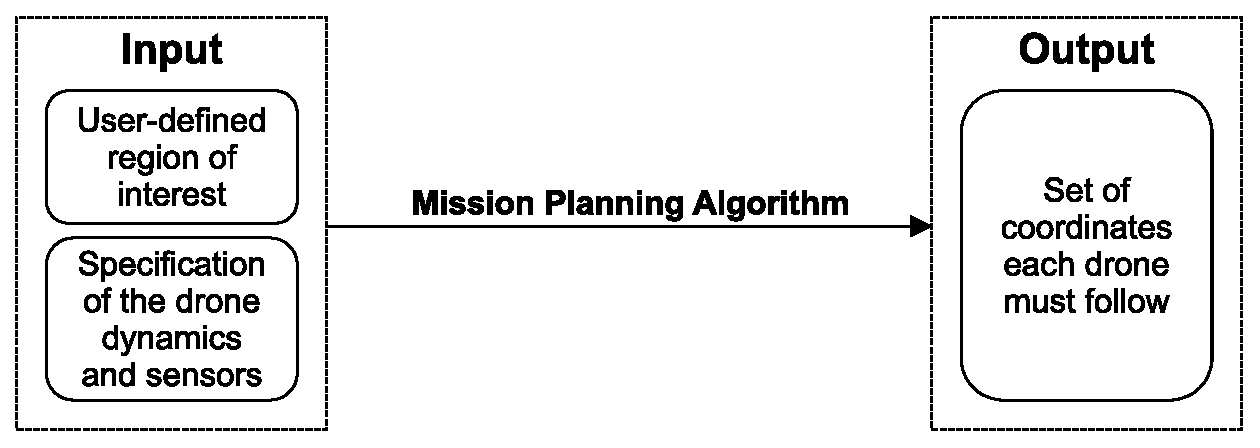
\includegraphics[width=0.7\linewidth]{figs/Jihwan/Objective of the Mission Planning System.eps}
    \caption[Objective of the Mission Planning System]
    {Objective of the mission planning system.}
    \label{fig:msp_objective}
\end{figure}

To have a successful mission planning framework, we wish to meet the following criteria:

\begin{itemize}
    \item \textbf{Efficiency}: The system should be efficient in terms of time, resource and cost compared to previous manual demining methods. 
    \item \textbf{Expandability}: The system should be expandable to a larger area of land by adding additional drones and base stations as necessary. 
    \item \textbf{Intuitiveness}: The system should be easily usable by the members of demining organisations even without professional software knowledge. 
\end{itemize}

This section will explain the theoretical basis of how the mission planning algorithm works for a single-drone system and demonstrate how it meets the criteria above through a real location example. Then, we explain how this algorithm will be expanded into a multi-drone system. Finally, the mission planning algorithm is compared to traditional mine detection methods to evaluate from the criteria above.  

%%%%%%%%%%
\subsection{Layered Approach}
\label{sec:msp_layered_approach}

\subsubsection{Algorithm Outline}

As mentioned in Section~\ref{sensor_hardware_data_acquisition}, we utilise thermal and \gls{GPR} sensors to detect the landmines. Table~\ref{tab:thermal_vs_gpr} illustrates the trade-off between thermal and \gls{GPR} sensors: a thermal sensor is able to scan at a higher altitude and fast speed which results in a shorter time to survey the given \gls{roi}, but a \gls{GPR} sensor results in a higher confidence in the mine location. 

\begin{table}[h!]
    \centering
    \begin{tabular}{| c || c | c |}
        \hline
        Sensor & Thermal & \gls{GPR} \\
        \hline\hline
        Altitude & \textbf{High} & Low \\
        \hline
        Speed & \textbf{Fast} & Slow \\
        \hline
        Confidence & Low & \textbf{High} \\
        \hline
    \end{tabular}
    \caption[Comparison of Thermal and GPR Sensors]
    {Comparison of thermal and \gls{GPR} sensors. Bold entries indicate a comparative advantage.}
    \label{tab:thermal_vs_gpr}
\end{table}

The layered approach aims to optimise between this trade-off by structuring the mission planning algorithm into 6 steps: \textbf{Define}, \textbf{Cover}, \textbf{Analyse}, \textbf{Target}, \textbf{Confirm} and \textbf{Demine}. 

\begin{enumerate}
    \item \textbf{Define}: The \gls{roi} and its obstacles are defined using a \gls{gis} software by the system operator. (Section~\ref{sec:msp_define})
    \item \textbf{Cover}: The \gls{roi} is fully covered by the thermal sensor in a Boustrophedon (back-and-forth) path through a \gls{cpp} algorithm. (Section~\ref{sec:msp_cpp})
    \item \textbf{Analyse}: The resulting thermal sensor readings are analysed by a machine learning algorithm to return a list of suspected landmine points. (Section~\ref{computervision}) 
    \item \textbf{Target}: The suspected landmine points are targeted and rescanned by the \gls{GPR} sensor in a minimum traversal path through a \gls{tspo} algorithm. (Section~\ref{sec:msp_tspo}) 
    \item \textbf{Confirm}: The resulting \gls{GPR} readings are analysed by a machine learning algorithm to return the final result on the locations of the landmines. (Section~\ref{computervision})
    \item \textbf{Demine}: The \gls{roi} is demined based on the generated landmine location map. The demining operation itself is outside the scope of this project, and it will be the responsibility of the demining organisations to safely deactivate and remove the mines.
\end{enumerate}

% add a diagram for summarising the layered approach?

%%%%%%%%%%
\subsection{Defining the Region of Interest}
\label{sec:msp_define}

\subsubsection{Geometric Representation}

The \gls{roi} is an abstract representation of the minefield we wish to survey using our multi-aerial drone system. To apply geometric operations as required by the mission planning algorithm, we represent the \gls{roi} as a Polygon with Holes class (\texttt{Polygon\_with\_holes\_2}) from the \gls{cgal}\footnote{\url{https://www.cgal.org/}} which defines the outer boundary and its holes (obstacles) as a set of vertex coordinates \cite{cgal2024pwh}. \gls{cgal} provides various algorithms that can be directly applied to a Polygon with Holes object -- some of them will be explored and applied in later sections to construct the mission planning algorithm. Throughout the report (Figures \ref{fig:msp_straight_skeleton}, \ref{fig:msp_bahnemann}, \ref{fig:msp_tspo_20_100}, \ref{fig:msp_tspo_plot} and \ref{fig:msp_cdt}), an example Polygon with Holes object extracted from \cite{bahnemann2021cpp} based on a dataset by \cite{sun2014dataset} will be used to represent a simple \gls{roi} with a square outer boundary of width 100\,m. 

\subsubsection{Geographic Information System}

\gls{gis} software connects the geometric representation of the \gls{roi} to a geographic map in an accessible user-interface. This project uses a free and open-source \gls{gis} software called \gls{qgis}\footnote{\url{https://qgis.org/}} from which the demining operator can define the \gls{roi}. The process of defining the \gls{roi} on \gls{qgis} is shown in Figure~\ref{fig:msp_qgis}. Once all the outer polygon and its holes have been created to define the full \gls{roi}, the operator can export the coordinates in a GeoJSON\footnote{\url{https://geojson.org/}} format which gets converted into a Polygon with Holes object.

% add notes on satellite source and mapping drone?

\begin{figure}[h!]
    \centering
    \begin{tabular}{cc}
        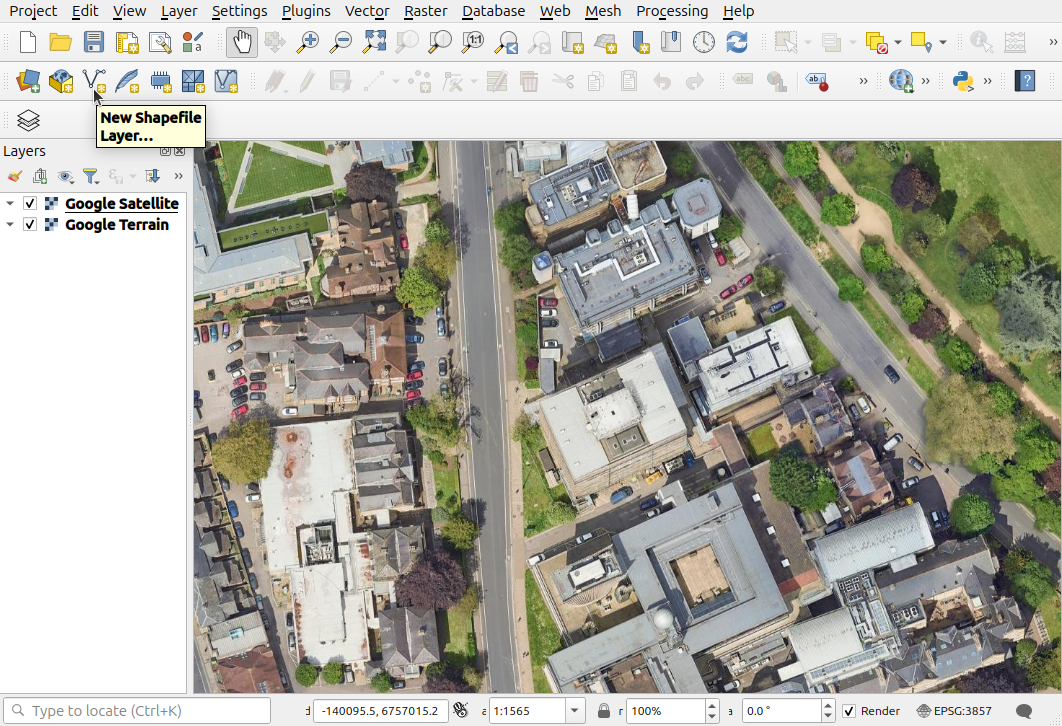
\includegraphics[width=0.45\textwidth]{figs/Jihwan/qgis_a.png} &
        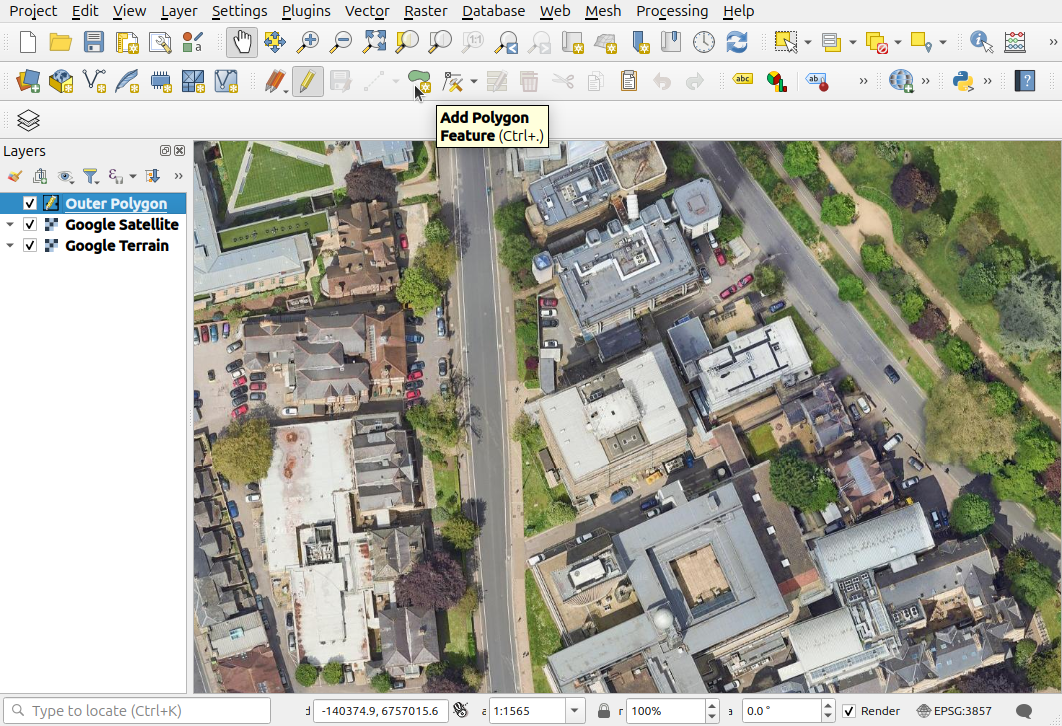
\includegraphics[width=0.45\textwidth]{figs/Jihwan/qgis_b.png} \\
        (a) & (b) \\[10pt]
        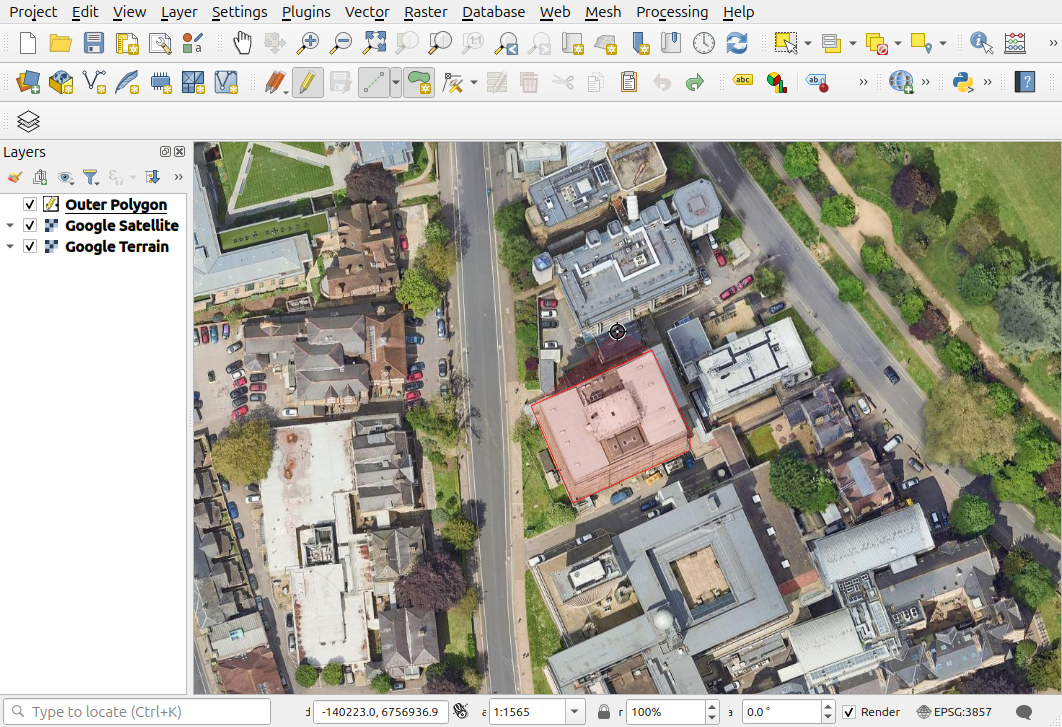
\includegraphics[width=0.45\textwidth]{figs/Jihwan/qgis_c.png} &
        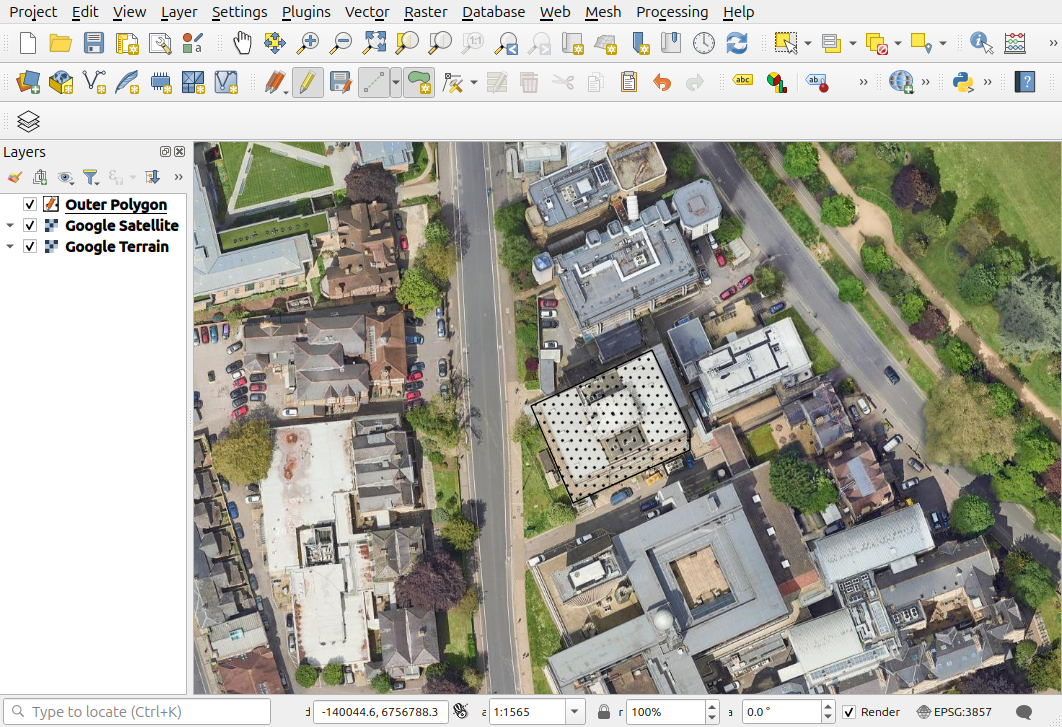
\includegraphics[width=0.45\textwidth]{figs/Jihwan/qgis_d.png} \\
        (c) & (d)
    \end{tabular}
    \caption[Demonstration of ROI Definition using QGIS]
    {Demonstration of defining the \gls{roi} using \gls{qgis}. (a) New Shapefile layer is created. (b) New polygon feature named "Outer Polygon" is defined. (c) The system operator marks the vertices of the polygon. (d) The final polygon is displayed. Additional polygons can be added to define the full \gls{roi}.}
    \label{fig:msp_qgis}
\end{figure}

% add note on coordinate system? qgis uses epsg:3857 but it can be changed. 

\subsubsection{Boundary Offset}

In some cases, it may be necessary to ensure that the drones do not exit the \gls{roi} or approach any of its internal obstacles. To do so, a boundary offset can be introduced using the straight skeleton algorithm as suggested in \cite{shahid2024cpp}. The straight skeleton of a polygon can be found by a shrinking process in which the boundary is contracted towards the interior in a self-parallel manner and at the same speed for all edges \cite{aichholzer1996ss}. Applying the shrinking process by a specified length would result in an internal boundary offset of the original polygon. \gls{cgal} provides an implementation for the straight skeleton algorithm in its 2D Straight Skeleton and Polygon Offsetting package which can be directly applied to a Polygon with Holes object \cite{cgal2024ss}.

Figure~\ref{fig:msp_straight_skeleton} shows the result of applying \gls{cgal}'s straight skeleton algorithm to obtain the offset of the \gls{roi} boundary. It shows a successful generation of the boundary offset even for complex geometries, validating this approach for the use case. Furthermore, the size of the offset can be varied depending on the requirements of the mission. 

\begin{figure}[h!]
    \centering
    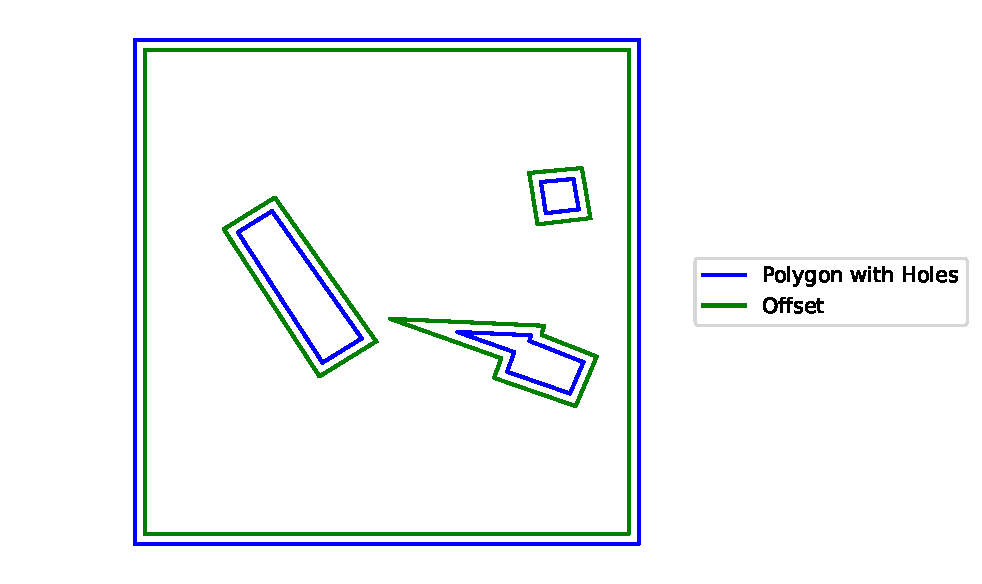
\includegraphics[width=0.6\linewidth]{figs/Jihwan/Polygon Offset with Straight Skeleton.pdf}
    \caption[Offset of ROI using Straight Skeleton]
    {A 2\,m offset of a Polygon with Holes has been generated using \gls{cgal}'s straight skeleton method.}
    \label{fig:msp_straight_skeleton}
\end{figure}

%%%%%%%%%%
\subsection{Coverage Path Planning}
\label{sec:msp_cpp}

\gls{cpp} is a task in which an agent (drone) must cover every point in the given environment (\gls{roi}) with its method of action (thermal sensor reading). To obtain the solution of a \gls{cpp} problem, the \gls{roi} is first decomposed into smaller polygons. In large, this can be distinguished between \textit{approximate} and \textit{exact} cellular decompositions. In an approximate cellular decomposition the \gls{roi} is decomposed into a grid of same size and shape (often a square). Assuming that a single grid is smaller than the size of the sensor's field of view, visiting all grids would indicate a full coverage of the \gls{roi} except the areas which are lost during the approximation process. In contrast, an exact cellular decomposition divides the \gls{roi} into a set of non-intersecting cells which are covered by a continuous path of motion, covering the entire \gls{roi} without missing regions \cite{choset2001surveycpp}. 

For the purpose of a landmine detection system, it is important to use the exact cellular decomposition. This would ensure that no landmines that could cause a safety hazard for the demining individuals have been missed out. In particular, this project uses the \gls{bcd} and path planning method that has been implemented by \cite{bahnemann2021cpp} which will be explained in detail below.  

\subsubsection{Boustrophedon Cellular Decomposition and Path Planning}

\gls{bcd} is an exact cellular decomposition method first proposed by \cite{choset1998bcd}. It stems from \gls{tcd} -- a straight line segment sweeps through the decomposition area in one direction, dividing the area into trapezoidal cells each time it passes through a vertex of the obstacle polygons (Figure~\ref{fig:msp_choset}a). \gls{bcd} reduces the number of cells created by merging trapezoidal cells which occur between \textit{IN} (the straight line segmented is divided into two by the obstacle) and \textit{OUT} (the straight line segments are merged into one after passing the obstacle) events (Figure~\ref{fig:msp_choset}b). Having a fewer number of cells helps avoid unnecessary overlapping swaths from being generated in between two neighbouring cells as demonstrated in Figure~\ref{fig:msp_choset}c. 

\begin{figure}[h!]
    \centering
    \begin{tabular}{p{0.3\textwidth}p{0.3\textwidth}p{0.3\textwidth}}
        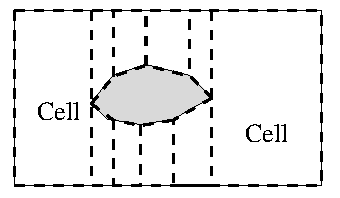
\includegraphics[width=0.3\textwidth]{figs/Jihwan/choset_tcd.pdf} &
        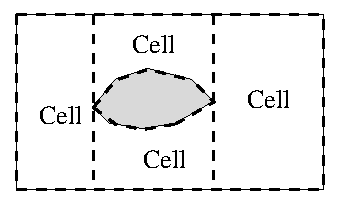
\includegraphics[width=0.3\textwidth]{figs/Jihwan/choset_bcd.pdf} &
        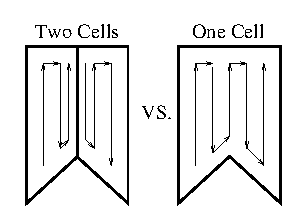
\includegraphics[width=0.3\textwidth]{figs/Jihwan/choset_bcd_tcd_comparison.pdf} \\
        \centering (a) Resulting cells from \gls{tcd} giving 10 cells. & 
        \centering (b) Resulting cells from \gls{bcd} giving 4 cells. & 
        \centering (c) Comparison of coverage paths using \gls{tcd} (left) and \gls{bcd} (right).
    \end{tabular}
    \caption[Comparison between TCD and BCD]
    {Comparison between \gls{tcd} and \gls{bcd} adapted from \cite{choset1998bcd}.}
    \label{fig:msp_choset}
\end{figure}

In each cell, boustrophedon (back-and-forth) paths are generated for the drone to cover the region with its sensor. Based on the thermal sensor decided in Section~\ref{thermal_system}, the coverage width of the drone travelling in a straight line is approximately 9\,m. A set of parallel lines are drawn within the boundary of the cell with spacings equal to the coverage width. The end of these parallel lines are then connected appropriately to generate the continuous path the drone must take to fully cover the cell with its sensor's \gls{FOV}. Based on the angle at which the parallel lines are drawn, the coverage path can be optimised with respect to two different loss functions: the total distance travelled or the number of turns taken (as turning is a costly manoeuvrer compared to a straight path, so it should be minimised). The method for finding the optimal angle for convex and non-convex polygons is discussed in \cite{torres2016cpp} which in brief involves finding the maximum width of the cell's convex hull. 

The boustrophedon paths of each cell should now be connected to form a continuous path across all cells in the decomposition. This can be done by the use of an adjacency graph \cite{choset1998bcd}. An undirected graph is initialised where each cell of the decomposition corresponds to a node. Edges are created between cells which are adjacent to one another (two cells share one or more edges) where the weight is the distance between the end of one cell's coverage path to the start of the other cell's coverage path. The \gls{cpp} problem is now simplified into one in which the agent (drone) must visit all cells in the adjacency graph at least once, covering each cell with their individual boustrophedon paths. This is equivalent to a \gls{tsp}, for which the solutions will be explored in more detail in Section~\ref{sec:msp_tspo}. 

In the end, we are able to find a continuous path for the drone which is able to cover the entire \gls{roi}. The whole \gls{cpp} algorithm explained above is well-summarised by Figure~\ref{fig:msp_cabreira} from \cite{cabreira2019surveycpp}, which shows the full example of generating the coverage path of a \gls{roi} without any obstacles. The procedure for a \gls{roi} with obstacles is similar except for the fact that the connecting paths in between the cells may need to go around the obstacles.  

\begin{figure}[h!]
    \centering
    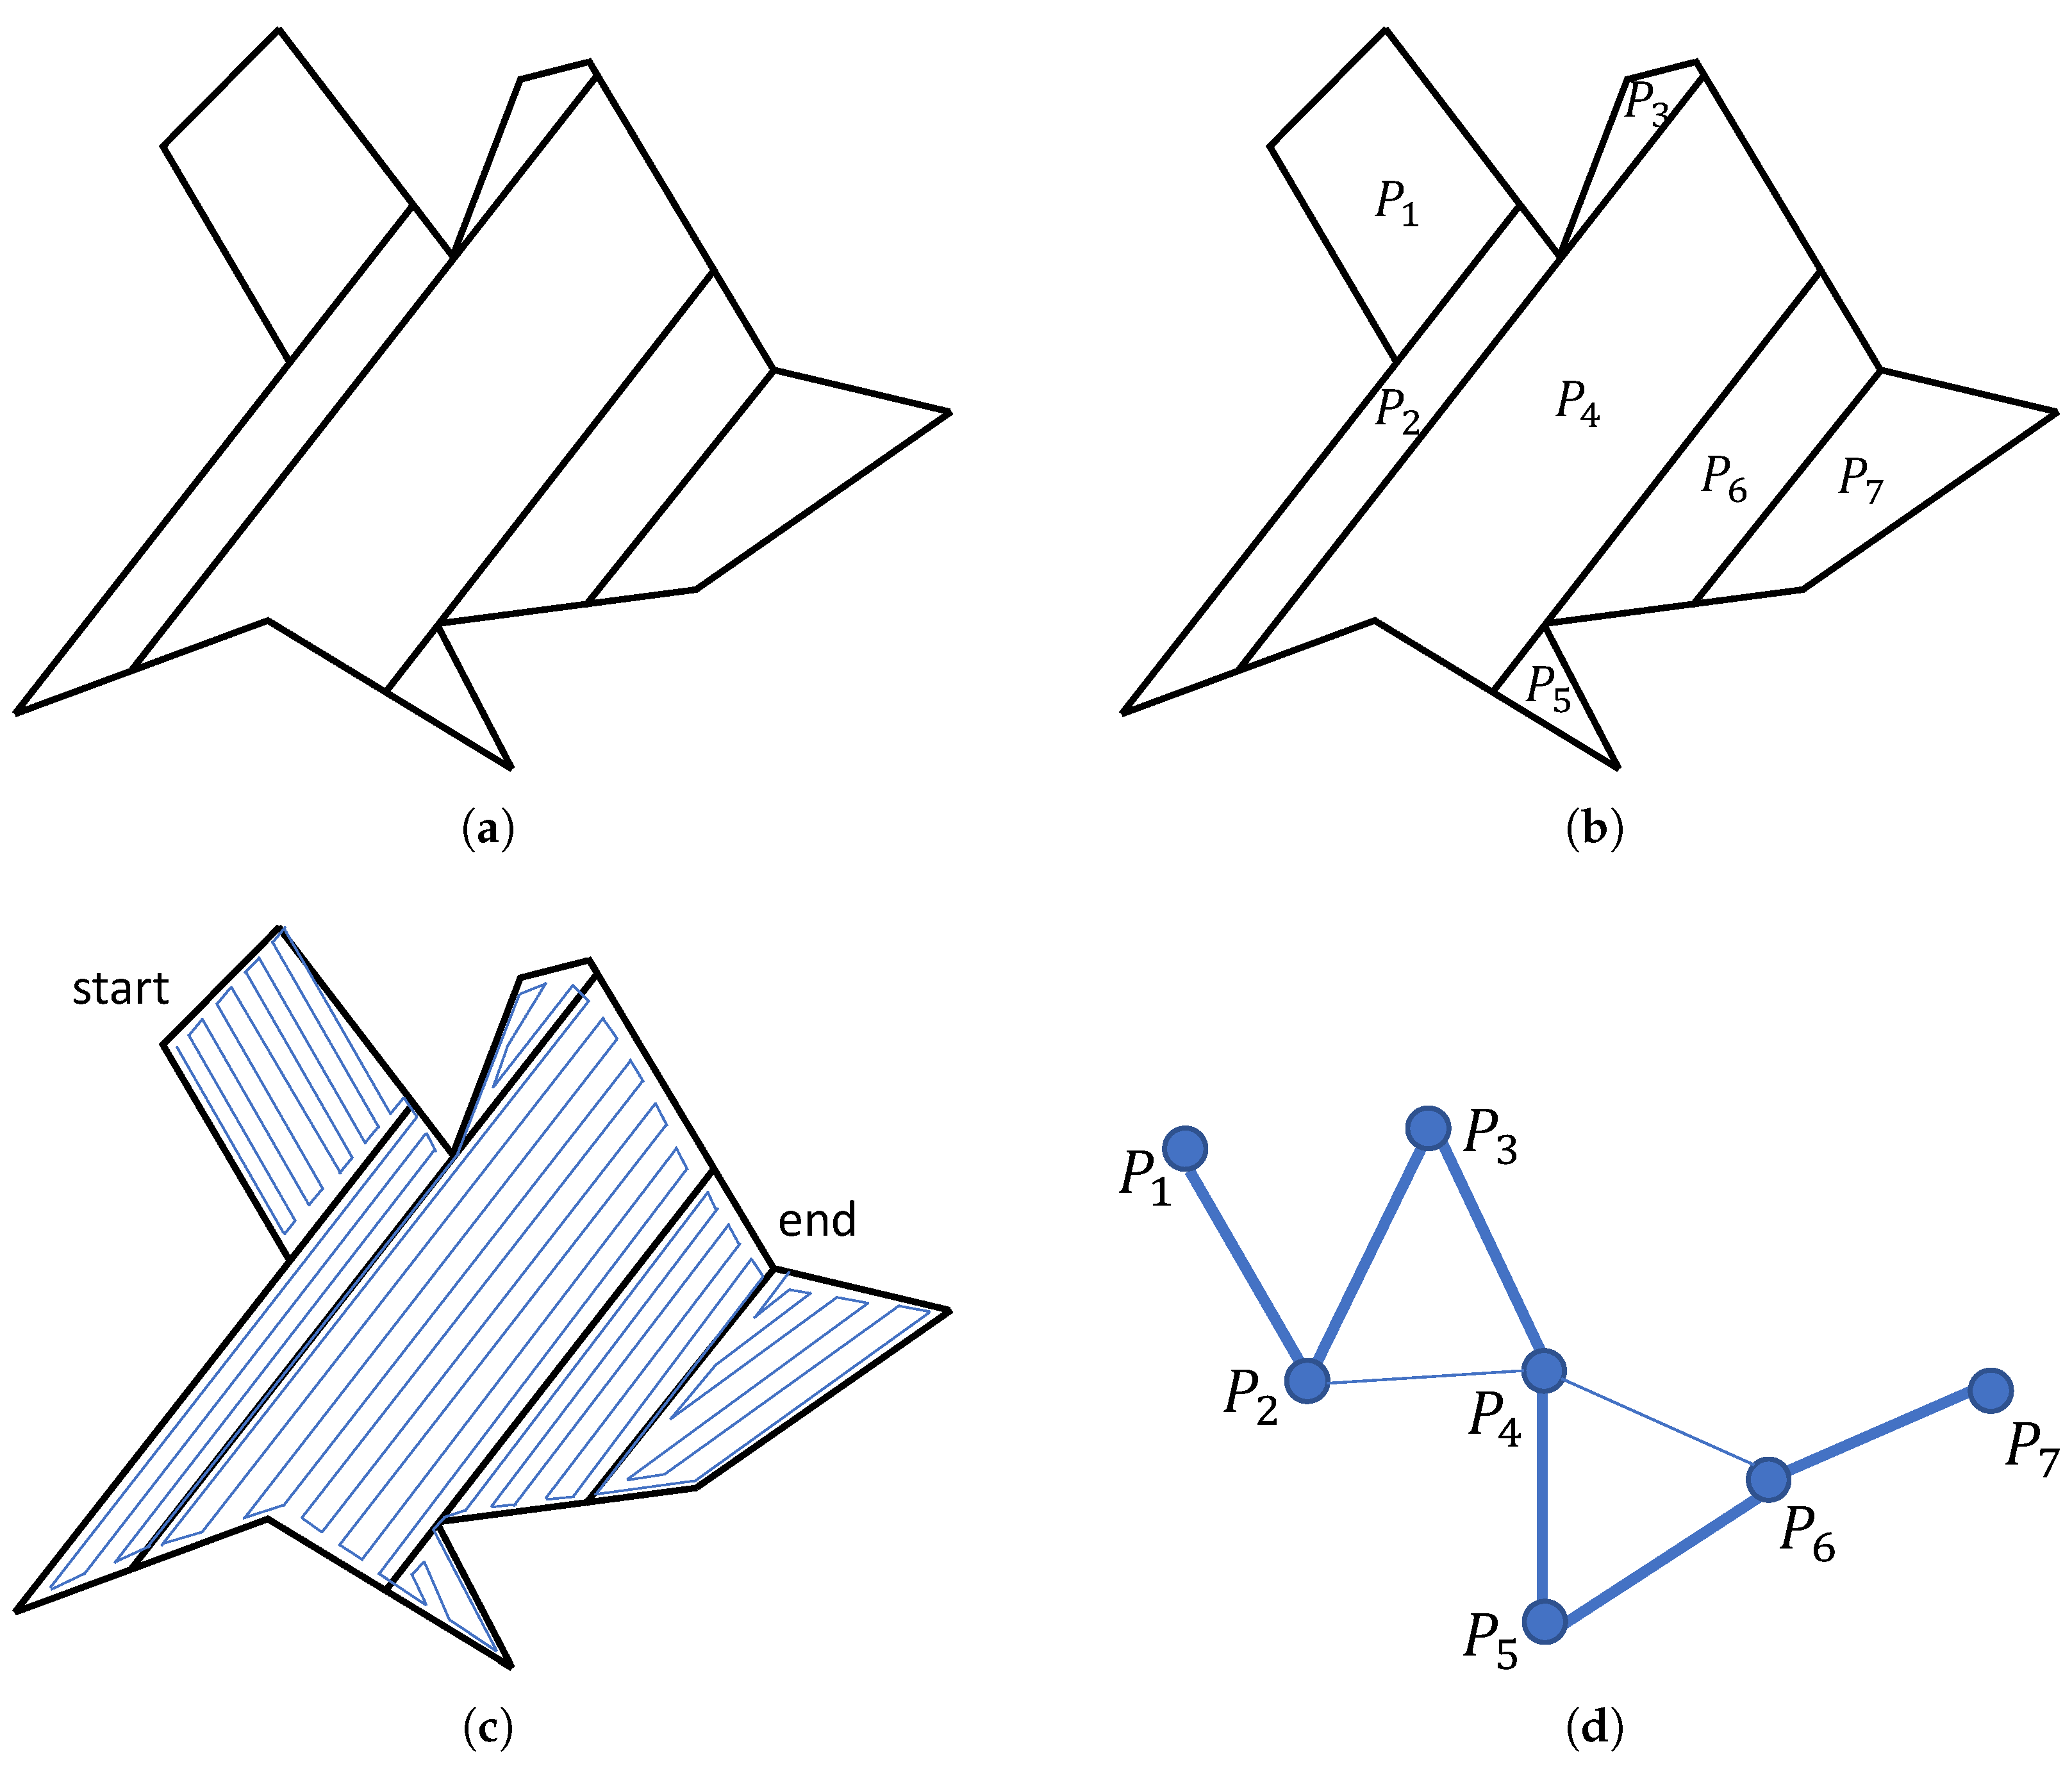
\includegraphics[width=0.7\linewidth]{figs//Jihwan/cabreira.png}
    \caption[Example of the Full CPP Algorithm]{Example of the full \gls{cpp} algorithm by \cite{cabreira2019surveycpp}. (a) The \gls{roi} is decomposed using \gls{bcd}. (b) Each cell is assigned as a node in the adjacency graph. (c) The boustrophedon paths of each cell is generated and connected based on the \gls{tsp} solution of the adjacency graph. (d) The \gls{tsp} solution of the adjacency graph is shown for clarity.}
    \label{fig:msp_cabreira}
\end{figure}

\subsubsection{Implementation}

To solve the \gls{cpp} problem, an implementation made by \cite{bahnemann2021cpp} (available on their GitHub repository ethz-asl/polygon\_coverage\_planning\footnote{\url{https://github.com/ethz-asl/polygon_coverage_planning/tree/master}}) is used. The program is subject to the GNU GPL-3.0 license\footnote{\url{https://www.gnu.org/licenses/gpl-3.0.en.html}} allowing commercial uses of copy, modification and distribution of the software given that it is subject to the same license. 

For use, the software must be compiled from its ROS Noetic\footnote{\url{https://wiki.ros.org/noetic}} packages on the Ubuntu 20.04 operating system. It allows for flexible customisation of the \gls{roi} as well as sensor specifications (drone height, sensor FOV angle, sensor coverage width, etc.) through the configuration files which can be run as ROS server requests. The output broadcasts the coverage path the drone must take in Cartesian coordinates, which can be converted and returned to the \gls{qgis} interface for approval by the demining operator. Figure~\ref{fig:msp_bahnemann} demonstrates the \gls{cpp} solutions for different sensor coverage widths found using the program. 

\begin{figure}[h!]
    \centering
    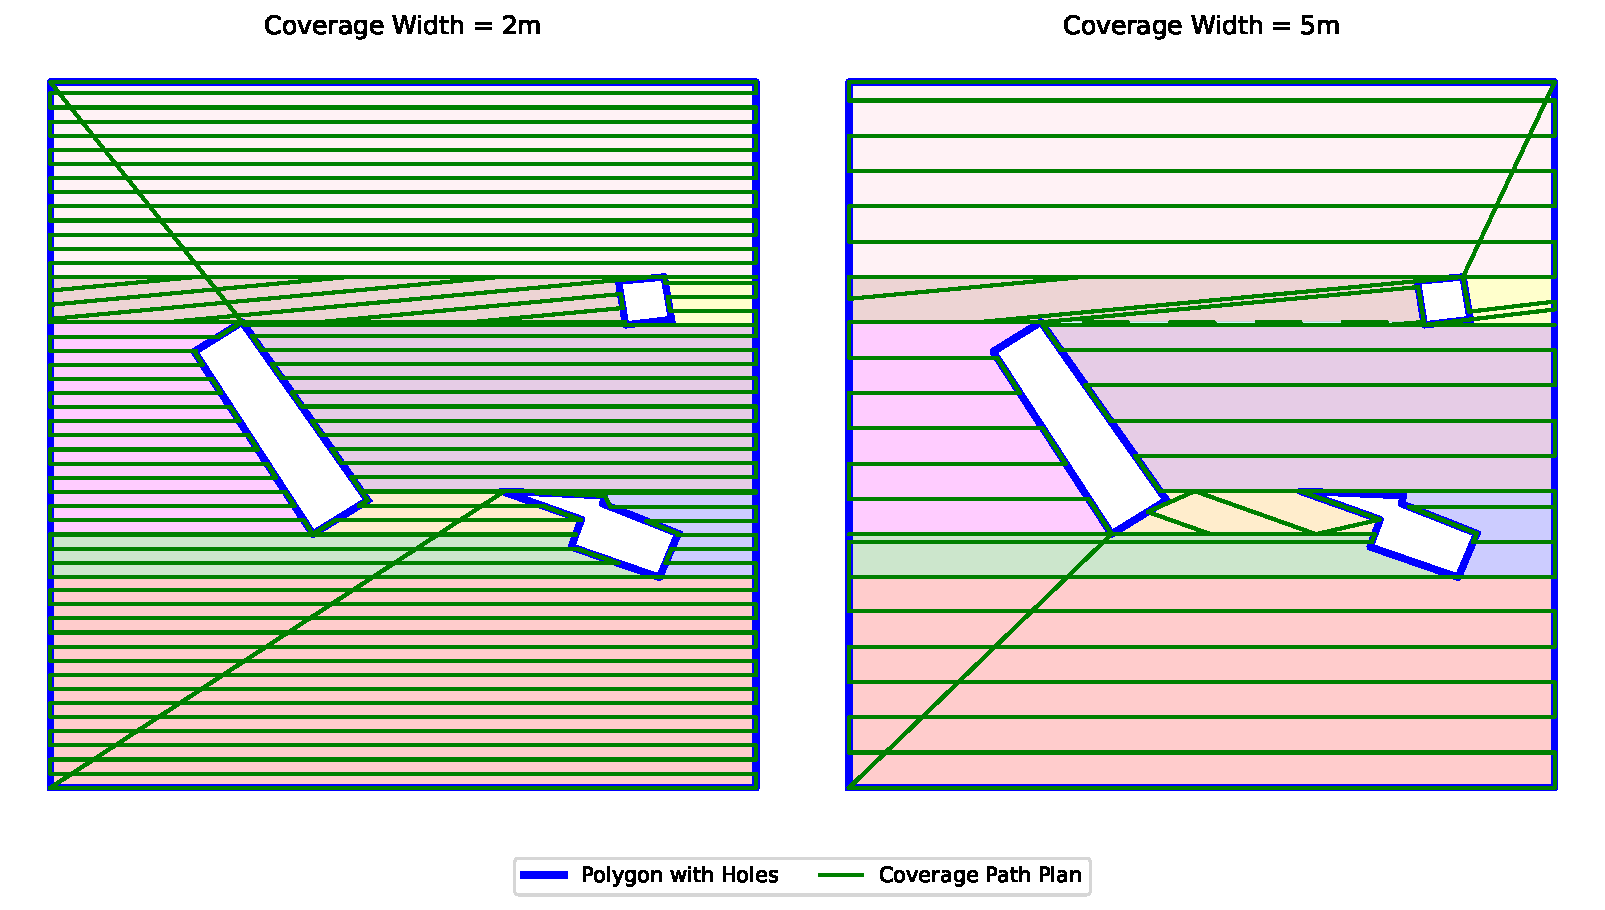
\includegraphics[width=\linewidth]{figs/Jihwan/CPP_diff_widths.pdf}
    \caption[CPP Solution Examples]
    {\gls{cpp} solutions have been found for sensor coverage widths of 2\,m (left) and 5\,m (right). The colour of the background indicates segmentations resulting from the \gls{bcd}.}
    \label{fig:msp_bahnemann}
\end{figure}

In this project, the software was compiled in a virtual machine (Multipass\footnote{\url{https://canonical.com/multipass}} Ubuntu 20.04 with NoMachine\footnote{\url{https://www.nomachine.com/}}) installed in an Ubuntu 24.01 host computer. The computational requirement of the software was sufficient to be run with this method, but in a real scenario it may be beneficial to port over the software as ROS2 Jazzy\footnote{\url{https://docs.ros.org/en/jazzy/index.html}} packages which can be run locally in the Ubuntu 24.01 host computer for a better integration with \gls{qgis} as well as other components of the layered approach. 

%%%%%%%%%%
\subsection{Travelling Salesman Problem with Obstacles}
\label{sec:msp_tspo}

\subsubsection{Travelling Salesman Problem}

The \gls{tsp} is an optimisation problem in which the minimum traversal path to visit all targeted nodes in a weighted graph must be found. A number of exact (optimal) and heuristic solutions have been studied and proposed as reviewed in \cite{laporte1992tsp} and \cite{zhang2023tsp}. Some of the methods have been compiled and compared in Table~\ref{tab:msp_tspcomparison}.  

\begin{table}[h!]
    \centering
    \begin{tabular}{|c|p{0.5\linewidth}|c|}
        \hline
        \textbf{Method} & \centering{\textbf{Explanation}} & \textbf{Complexity} \\
        \hline \hline
        Brute-Force Algorithm & Naïve method where all possible permutations are calculated to find the optimal solution. & $O(n!)$ \\ \hline
        Held-Karp Algorithm \cite{held1962hktsp} & Dynamic Programming method where subsets of nodes are explored to find the optimal solution. It improves on the brute-force method in terms of complexity while maintaining the optimal solution, but comes at the cost of large memory requirements. & $O(n^2 2^n)$ \\ \hline
        Genetic Algorithm \cite{potvin1996gentsp} & Searches for the heuristic solution by combining the best features of good solutions over multiple generations. & $O(n^2 g)$ \\ \hline
        Ant Colony Optimisation \cite{dorigo1997anttsp} & Mimics the behaviour of ants leaving pheromone trail (on edges of the graph) to successively shorten the path for a heuristic solution. & $O(n^2 m)$ \\ \hline
        Lin-Kernighan Algorithm \cite{lin1973lktsp} & Iteratively swap edges for local optimisation to find the heuristic solution. It is a popularly used method due to its performance and efficiency. & $O(n^2\log{n})$ \\ \hline
    \end{tabular}
    \caption[Comparison of TSP Solution Methods]
    {A comparison of \gls{tsp} solution methods. The complexity is expressed using Big O notation for the following variables: $n$ (number of nodes), $g$ (number of generations), $m$ (number of ants per iteration). The complexity may vary depending on the implementation.}
    \label{tab:msp_tspcomparison}
\end{table}

For the purpose of our layered approach, the number of suspected points will get large due to the size of the \gls{roi} and leniency towards high recall for the thermal sensor analysis algorithm (Section~\ref{compvis_intro}). It is also acceptable to sacrifice the optimality of the solution as it is not critical for surveying the \gls{roi} with the \gls{GPR} sensor. Hence, we choose the heuristic Lin-Kernighan algorithm for our problem. 

% more detailed explanation of the lk algorithm? 

The \gls{tsp} can be extended to more specific cases depending on the application, one of which is the \gls{tspo}. It introduces obstacles which the traversal path must avoid; this is exactly the problem that must be solved for the Target step of the layered approach, as the drone with a \gls{GPR} sensor must visit all suspected landmine points in the obstacle-filled \gls{roi}. The method for solving \gls{tspo} is explained in the next section. 

\subsubsection{Solving TSP-O using Visibility Graph}

One of the methods of solving a \gls{tspo} is to convert it into an ordinary \gls{tsp} using visibility graphs. A visibility graph is a data structure in which two nodes that are \textit{visible} (i.e. straight line segment between two nodes is not obstructed by any obstacles) are connected by an edge. In the context of geometric application like this project, the weight of the edge is defined to be the Euclidean distance between them. To check the visibility between two nodes on the 2D plane, \gls{cgal}'s 2D Visibility package \cite{cgal2024visibility} provides an implementation of the triangular expansion algorithm which can be applied on a Polygon with Holes object. By creating a visibility graph where all vertices of the \gls{roi} and the suspected landmine points are the nodes with visibility edges connecting them, the \gls{tspo} is simplified into an ordinary \gls{tsp} that can be solved using the \gls{tsp} solution listed in the previous section. This idea is explored in \cite{barb2024tspo} and \cite{bhat2024tspo} for more specific applications. 

The algorithm for converting a \gls{tspo} into a visibility graph given the Polygon with Holes $P$ and suspected (target) points $T$ is explained as pseudocode in Algorithm~\ref{alg:msp_tspo2visgraph}. It returns the visibility graph representation of the \gls{tspo}. The full process for solving the \gls{tspo} is visualised with a simple example in Figure~\ref{fig:msp_tspo}.

\begin{algorithm}[h!]
\caption{Creating the Visibility Graph of \gls{tspo}}
\label{alg:msp_tspo2visgraph}
\begin{algorithmic}[1]
\Require Polygon with Holes $P$, Set of target points $T = \{t_1, t_2, \ldots, t_q\}$ within $P$
\Ensure Visibility graph $G = (V, E)$

\State Initialize visibility graph $G = (V, E)$ with $V = \emptyset$ and $E = \emptyset$
\State $V \leftarrow T$ \Comment{Add all target points to the graph}
\State $V \leftarrow V \cup \text{Vertices}(P)$ \Comment{Add all vertices of polygon with holes to the graph}

\ForAll{$u \in V$}
    \ForAll{$v \in V$ where $u \neq v$}
        \If{$\text{IsVisible}(u, v)$}
            \State $E \leftarrow E \cup \{(u, v, d(u, v))\}$ \Comment{Add edge with Euclidean distance weight}
        \EndIf
    \EndFor
\EndFor

\Return $G$ \Comment{Return visibility graph}
\end{algorithmic}
\end{algorithm}

\begin{figure}[h!]
    \centering
    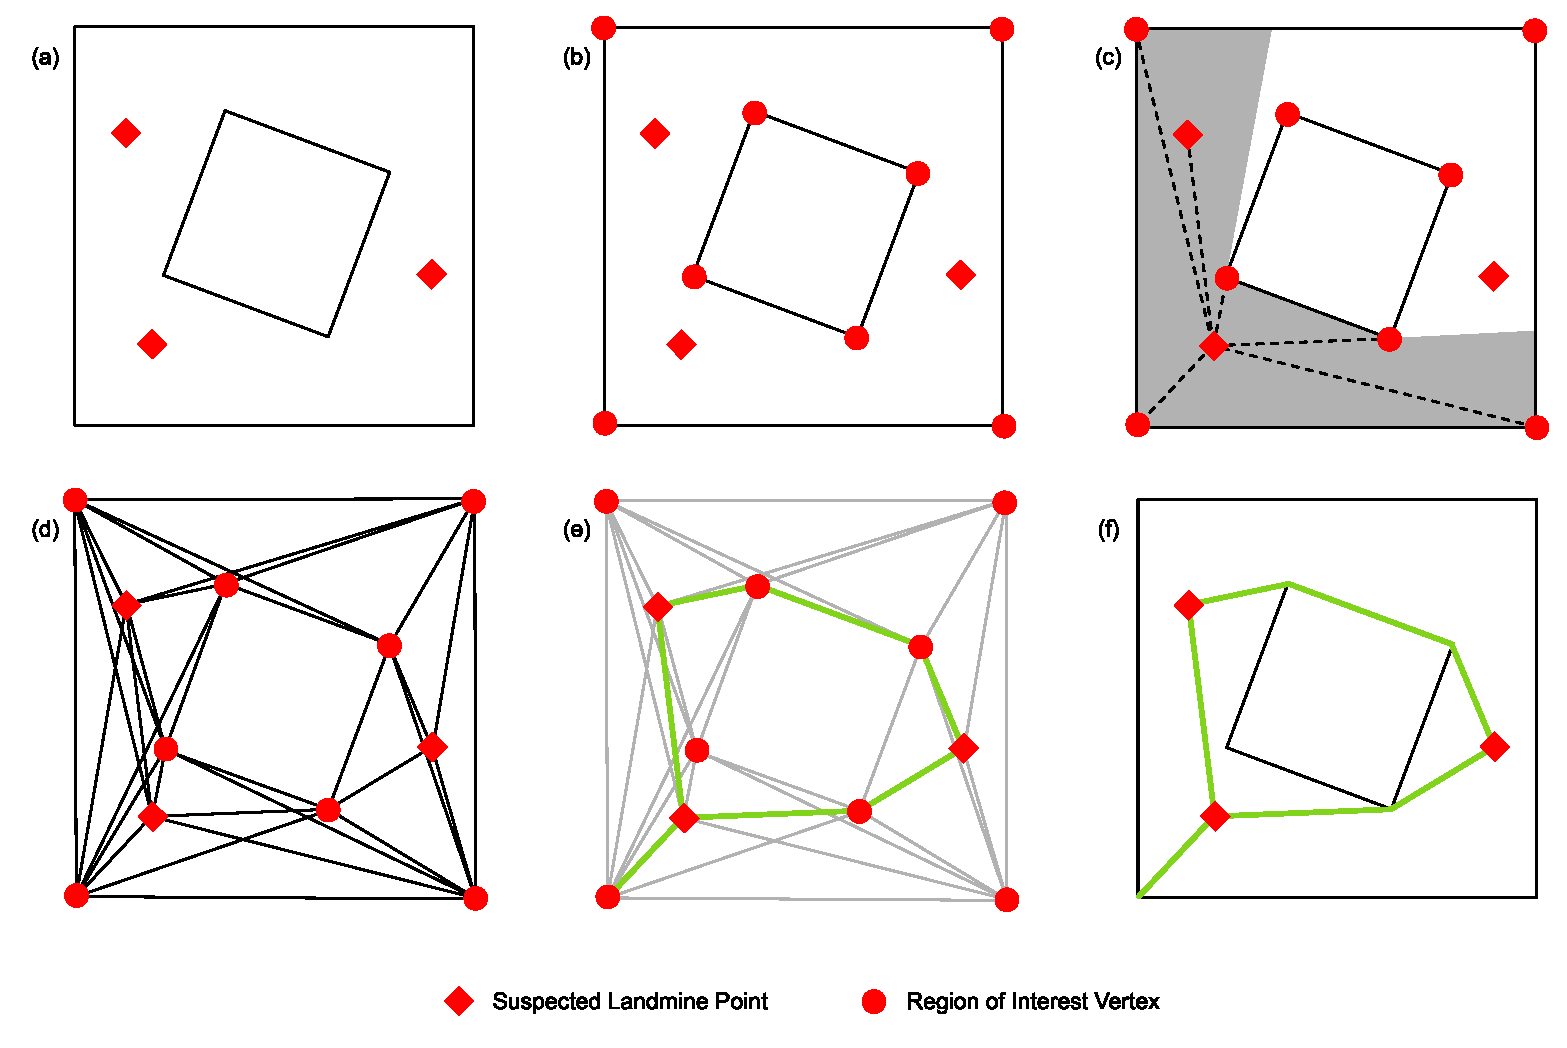
\includegraphics[width=\linewidth]{figs/Jihwan/TSPO Algorithm Visualisation.eps}
    \caption[TSP-O Algorithm Visualisation]
    {\gls{tspo} algorithm visualisation. (a) The example \gls{roi} is defined to have an outer boundary (outer square) with an obstacle (rotated inner square). Assume three suspected landmine points have been found from the Analyse step. (b) Add all suspected landmine points and \gls{roi} vertices as nodes to the visibility graph. (c) For each node, examine which other nodes are visible. Grey area indicates the visible region of the lower-left suspected landmine point. (d) Add weighted edges between visible nodes, with the weight being the Euclidean distance between them. The figure shows all connected edges between all nodes. (e) Perform a \gls{tsp} algorithm to visit all suspected landmine points in the visibility graph, starting from and ending at the base station. In this example, the lower left vertex of the outer boundary is defined as the base station. (f) Final solution of the minimal traversal path to visit all suspected landmine points is displayed, solving the \gls{tspo} algorithm. 
    }
    \label{fig:msp_tspo}
\end{figure}

\subsubsection{Time Complexity}

The time complexity of algorithm~\ref{alg:msp_tspo2visgraph} can be calculated to estimate the computing requirements for solving the \gls{tspo}. Note that the visibility condition is checked through the IsVisible($u$,$v$) function which is inside two nested for-loops iterating through all nodes in the visibility graph. Let $n$ be the number of nodes, which is equal to the sum of $p$ (the number of vertices in $P$) and $q$ (the number of points in $T$). In addition, let $h$ be the number of holes + 1. According to \cite{cgal2024visibility}, the time complexity for \gls{cgal}'s implementation of the visibility check (triangular expansion algorithm) is $O(n h)$. The nested for-loops will multiply $O(n)$ to the time complexity twice. Hence, the worst-case time complexity of Algorithm~\ref{alg:msp_tspo2visgraph} can be expressed as $O(n^3 h)$. 

The resulting visibility graph is then solved as an ordinary \gls{tsp} through the use of Lin-Kernighan algorithm explained above, which has the time complexity $O(n^2\log{n})$. Algorithm~\ref{alg:msp_tspo2visgraph} and the Lin-Kernighan algorithm are applied successively, meaning that their time complexities will be added to give $O(n^3 h + n^2\log{n})$. 

As $n$ increases to a large value, $O(n^2\log{n})$ becomes negligible compared to $O(n^3 h)$ in terms of its magnitude. The final time complexity of finding the solution to \gls{tspo} can therefore be expressed as $O(n^3 h)$. This is a reasonable value for computation given that the number of suspected landmine points does not come out to be too high for the \gls{roi}. 

% it will get too high, so we divide and cluster. 

\subsubsection{Implementation}

The \gls{tspo} was implemented using C++ based on the algorithms explained above, which gives the heuristic solution that cycles around the target points within a Polygon with Holes object. Figure~\ref{fig:msp_tspo_20_100} shows the computed solution for 20 and 100 randomly generated target points. They show near-optimal tour path confirming the validity of the implementation, exhibiting a behaviour in which the path wraps around the obstacles where necessary to achieve the minimum distance. This behaviour re-emphasises the need of a straight skeleton algorithm. 

Figure~\ref{fig:msp_tspo_plot} shows the effect of the number of target points on the computing time and total travel distance. The computing time rapidly increases as the number of target points passes 100 -- if the estimated computing time becomes too large, the operator may choose to divide the \gls{roi} into smaller subregions to reduce the total computing time. This would introduce an inefficiency in the total distance travelled by the drones, but it may become necessary due to the constraint of how much distance a single drone can cover before recharging. 

% add notes on how the implementation is sub-optimal and how it can be improved? would need to explain lin-kernighan in more detail first. 

\begin{figure}[h!]
    \centering
    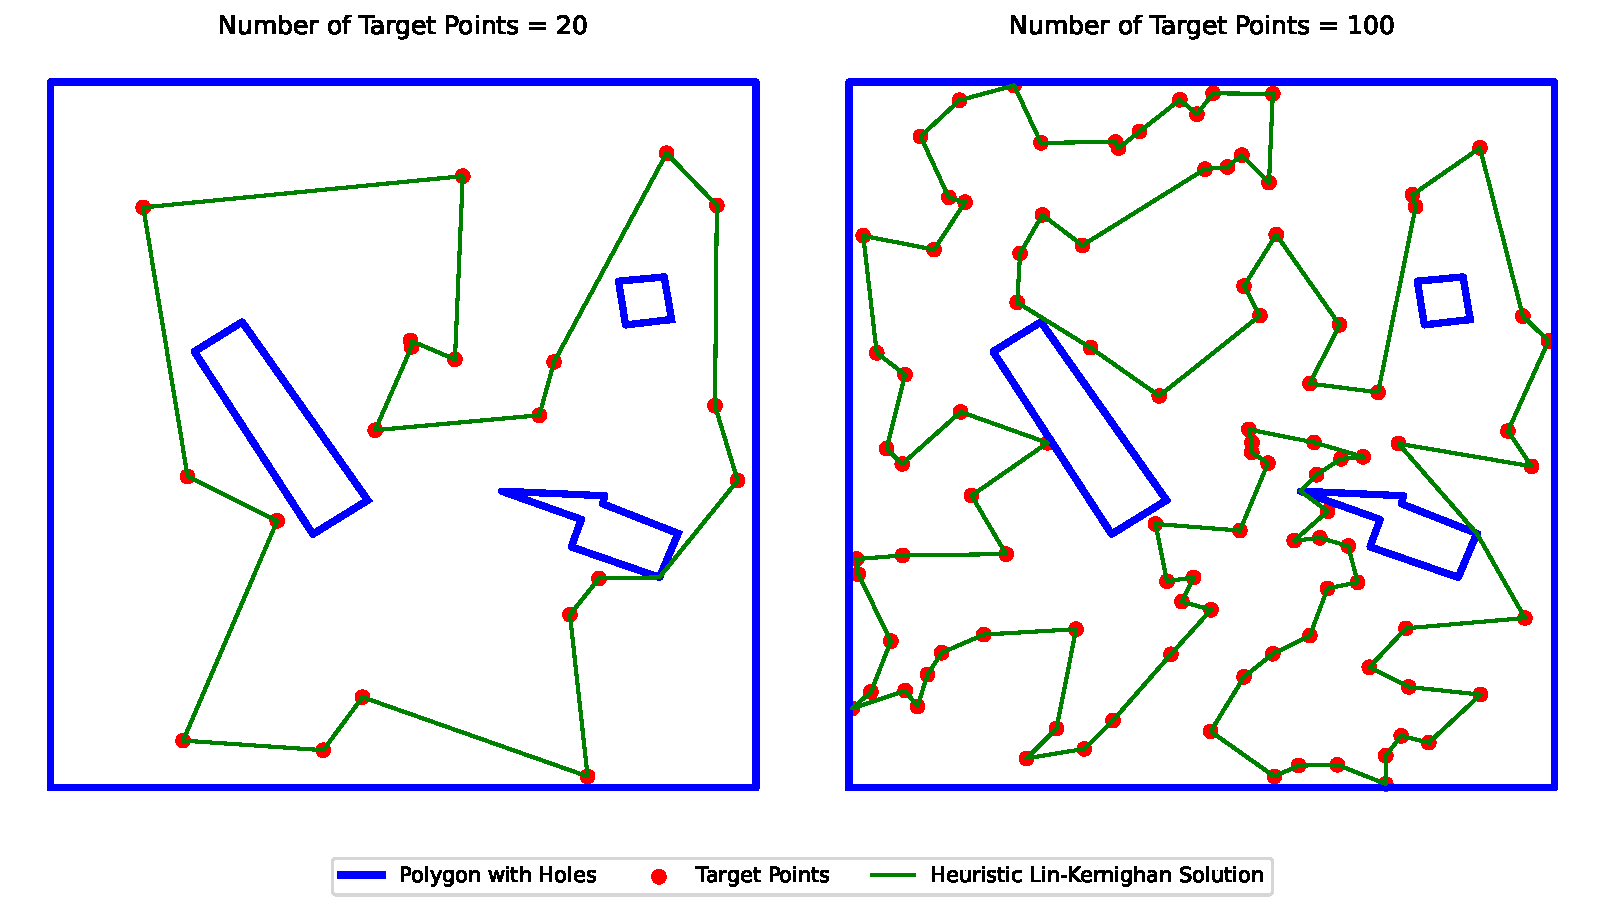
\includegraphics[width=\linewidth]{figs/Jihwan/TSPO_diff_targets.pdf}
    \caption[TSP-O Solution for Different Numbers of Target Points]
    {\gls{tspo} solutions have been generated for 20 (left) and 100 (right) target points randomly generated through rejection sampling.}
    \label{fig:msp_tspo_20_100}
\end{figure}

\begin{figure}[h!]
    \centering
    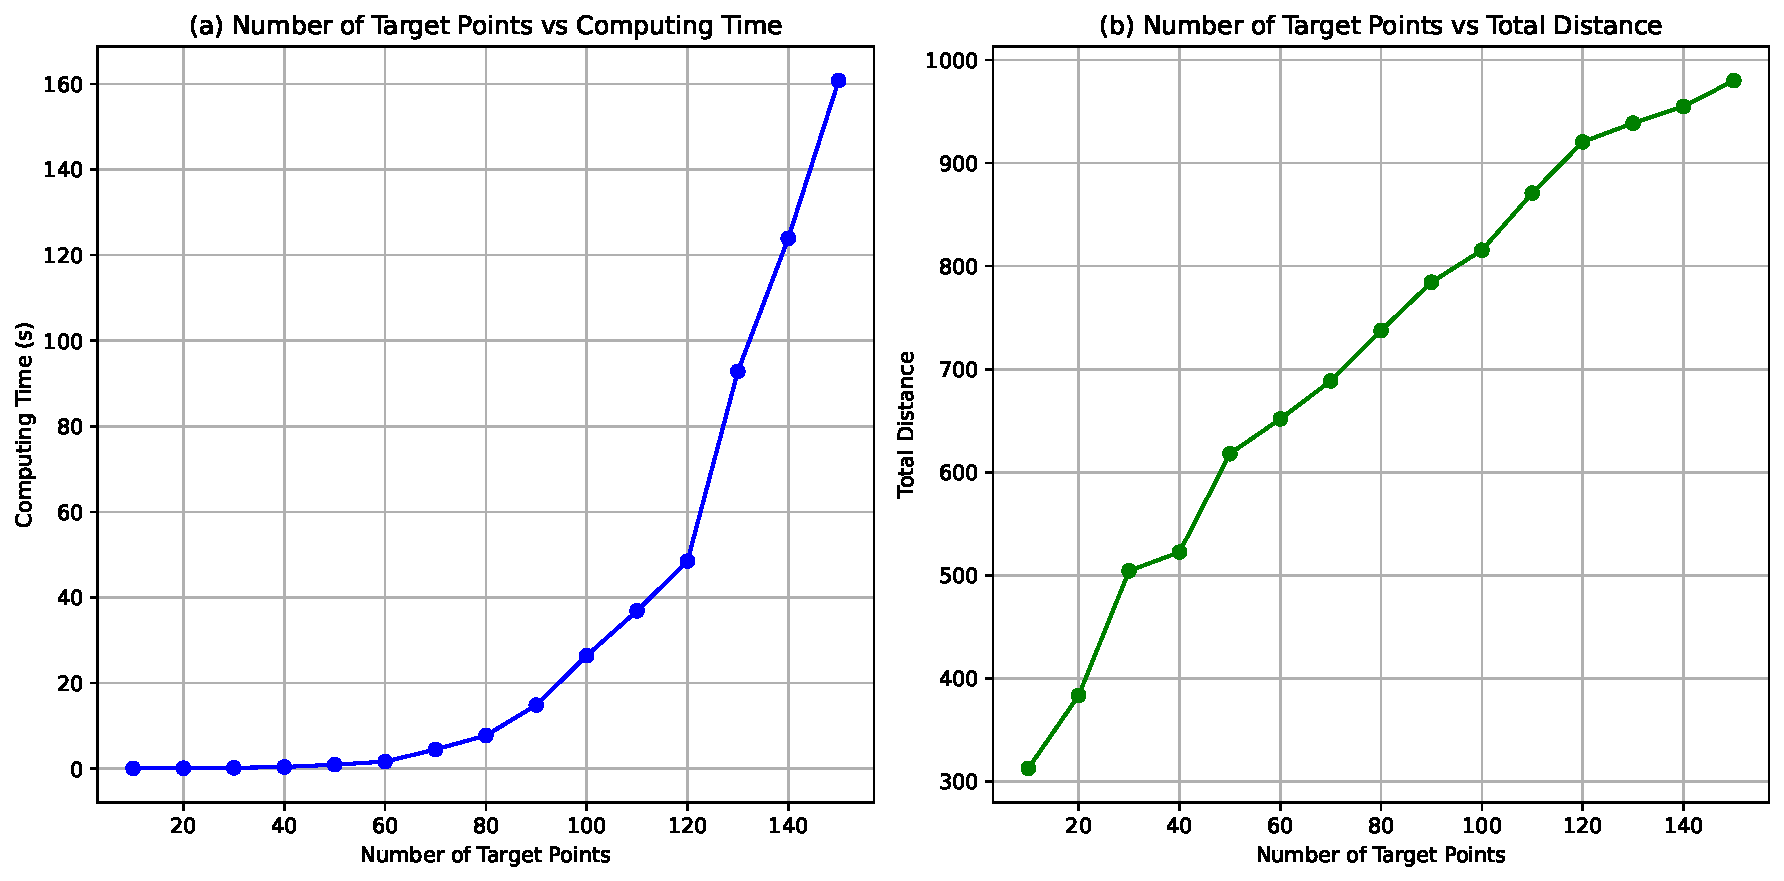
\includegraphics[width=\linewidth]{figs/Jihwan/target_points_vs.pdf}
    \caption[Effect of Number of Target Points on Computing Time and Total Distance of TSP-O Solution]
    {Plots showing the effect of the number of target points on the computing time (left) and total distance (right) in \gls{tspo}. Number of Target Points have been changed from 10 to 150 at increments of 10, taking the mean of 3 trials each where the target points are randomly generated through rejection sampling. The total distance is based on the scale where the width of the outer boundary is 100\,m.}
    \label{fig:msp_tspo_plot}
\end{figure}

%%%%%%%%%%
\subsection{Real Location Example}
\label{sec:msp_example}

To test the validity of the layered approach, a real location example has been conducted for an arbitrarily selected \gls{roi} at Ukraine (51°20'22.1"N 29°56'48.8"E) shown in Figure~\ref{fig:msp_example}a. The example demonstrates the Define, Cover and Target steps of the layered approach by displaying the results of each step on \gls{qgis}. 

\paragraph{Define} Figure~\ref{fig:msp_example}b shows the \gls{roi} defined using \gls{qgis}. The \gls{roi} is about the size of a 400\,m by 400\,m field with 3 obstacles which have been manually identified.  

\paragraph{Cover} Figure~\ref{fig:msp_example}c shows the \gls{cpp} solution found using the implementation by \cite{bahnemann2021cpp}. The coverage width has been specified as approximately 9\,m, and the start/end points have been arbitrarily decided to be at the top-right region outside the \gls{roi}. A thermal sensor drone will follow the generated path plan to collect the thermal readings. The total length of the path is calculated to be 15526\,m.

\paragraph{Target} Figure~\ref{fig:msp_example}d shows the \gls{tspo} solution found using Algorithm~\ref{alg:msp_tspo2visgraph} and the heuristic Lin-Kernighan algorithm. To represent the suspected landmine points, 20 coordinates within the \gls{roi} have been randomly generated using rejection sampling. The total length of the path is calculated to be 1777\,m. In a real mission, the suspected landmine points would be found during the Analyse step based on the thermal readings. At each point, the \gls{GPR} sensor drone will perform the scanning procedure described in Section~\ref{GPR_flight} before continuing onto the next point. 

For Cover and Target, if the total length of the path is too large to be covered by a single drone the operator may choose to deploy multiple drones to cover the \gls{roi}. This is further explained in Section~\ref{sec:msp_multi_drone}. 

\begin{figure}[h!]
    \centering
    \begin{tabular}{cc}
        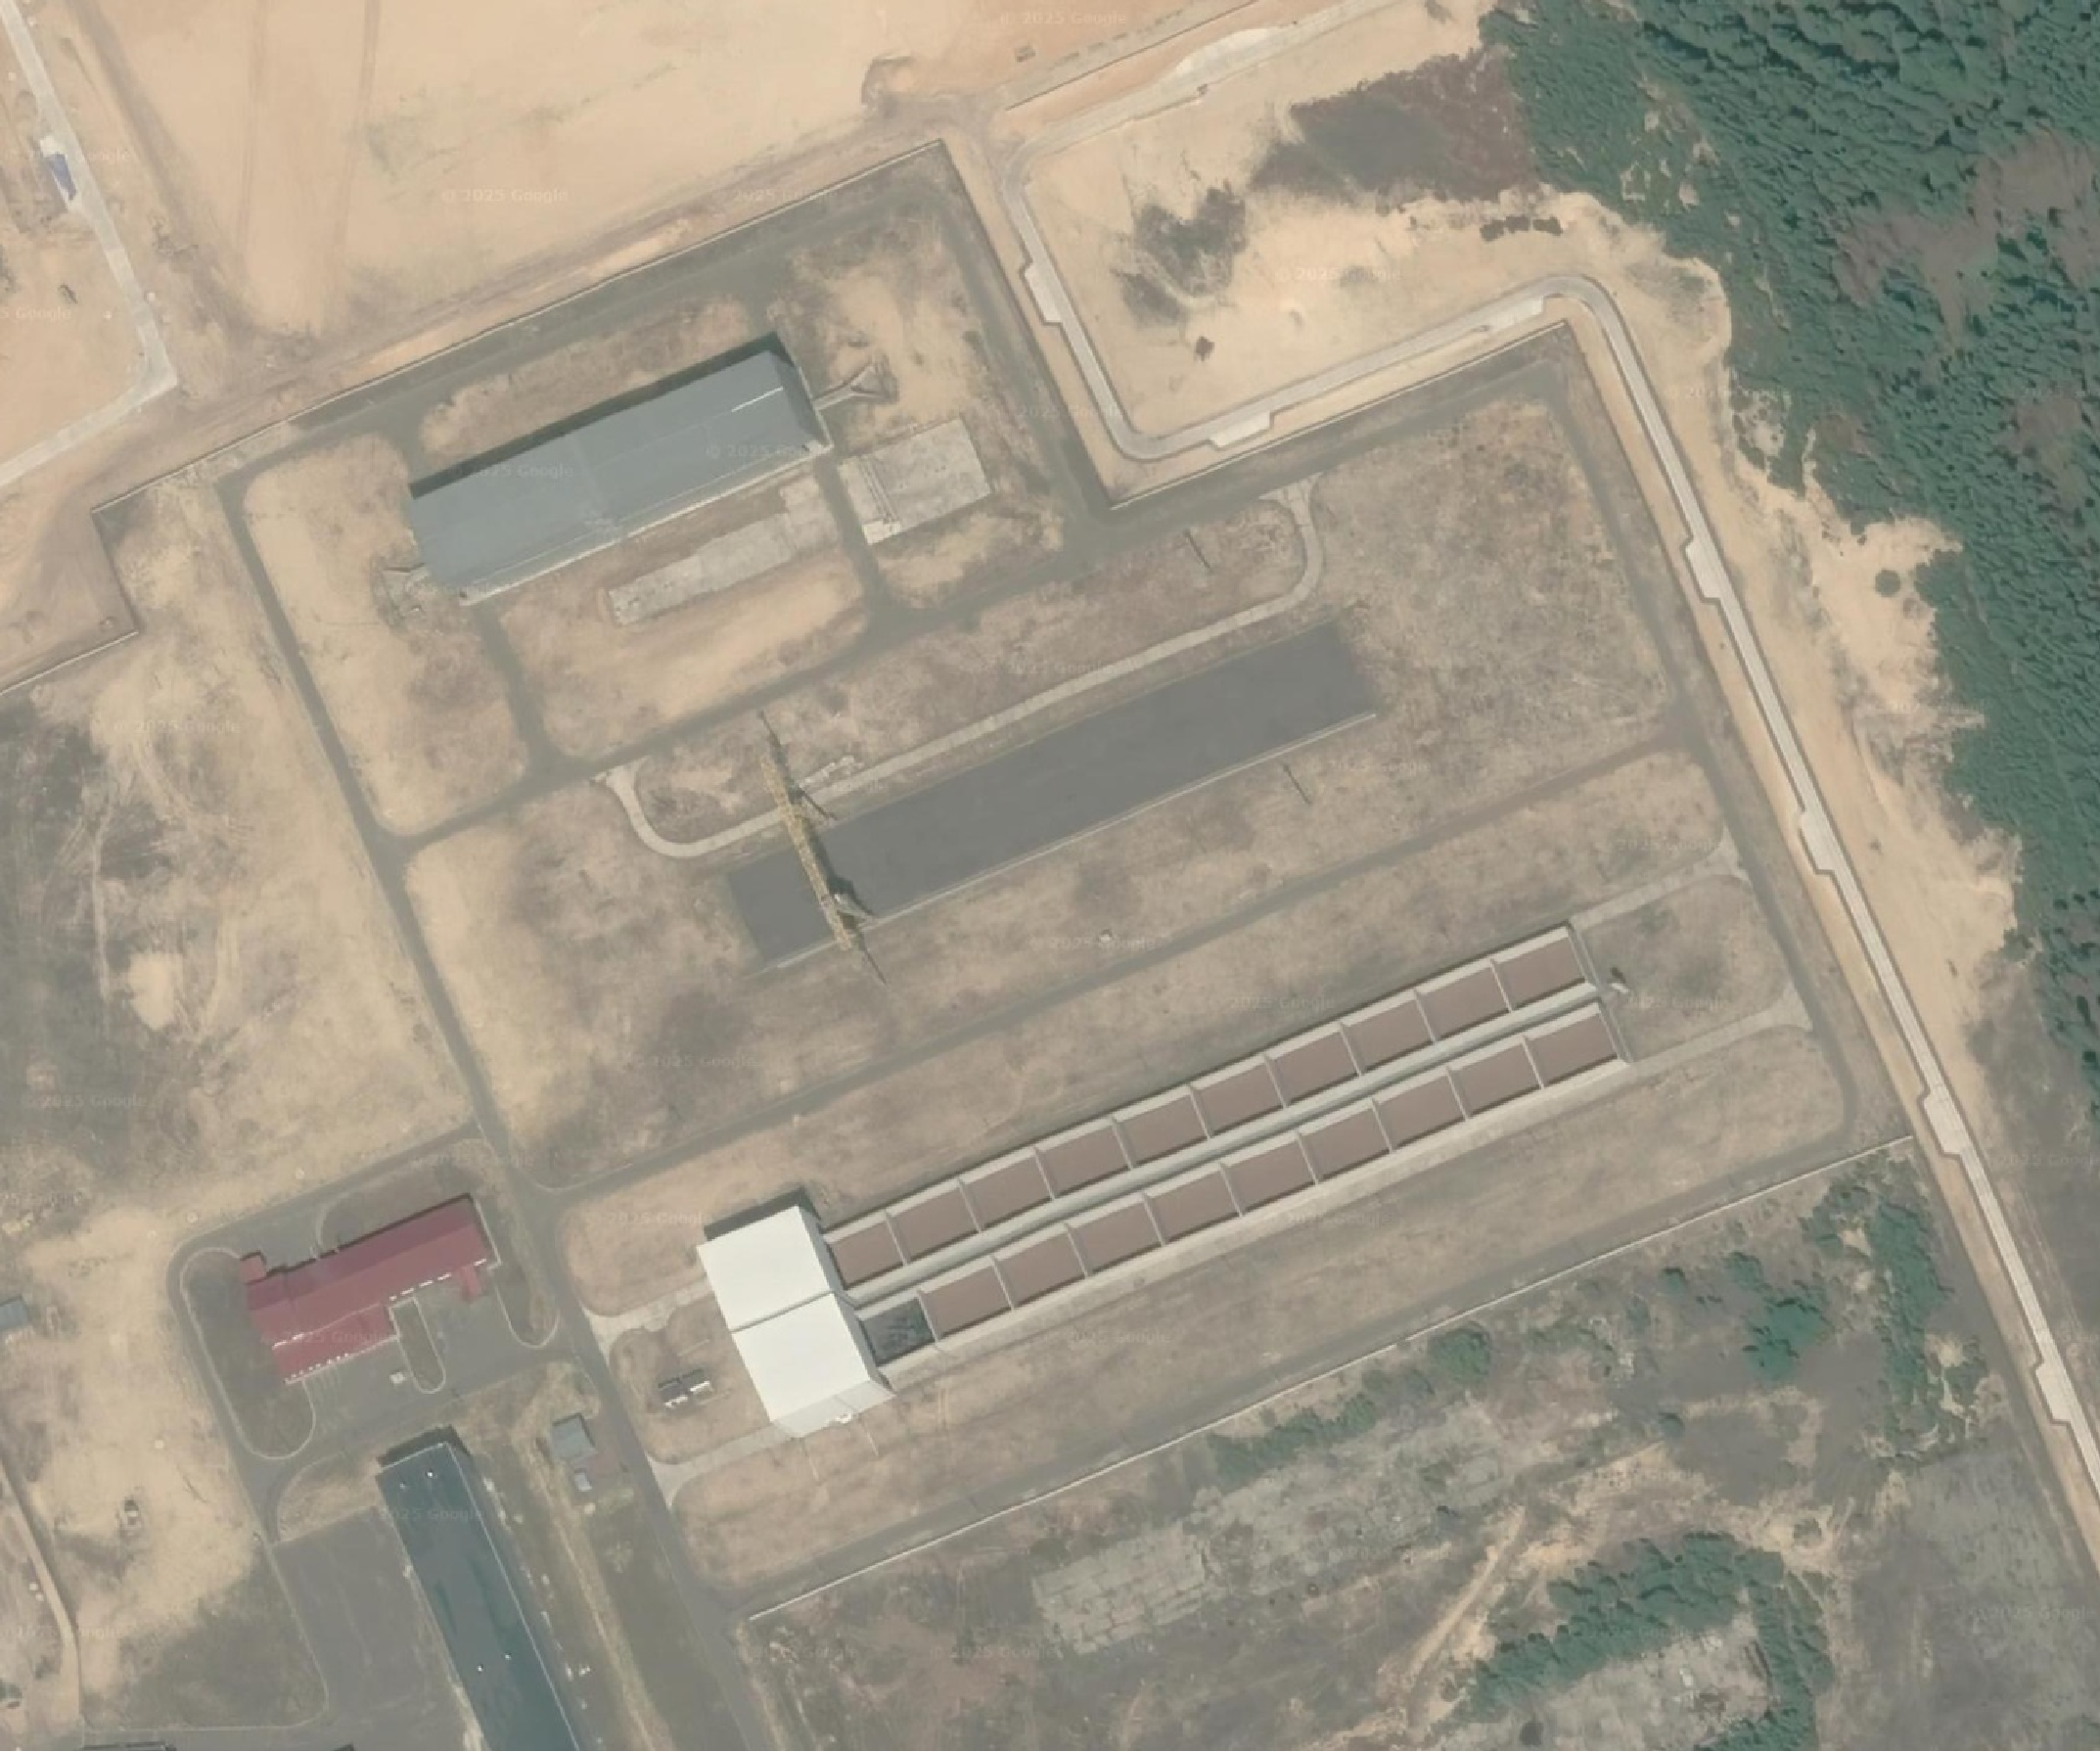
\includegraphics[width=0.45\textwidth]{figs/Jihwan/map1.pdf} &
        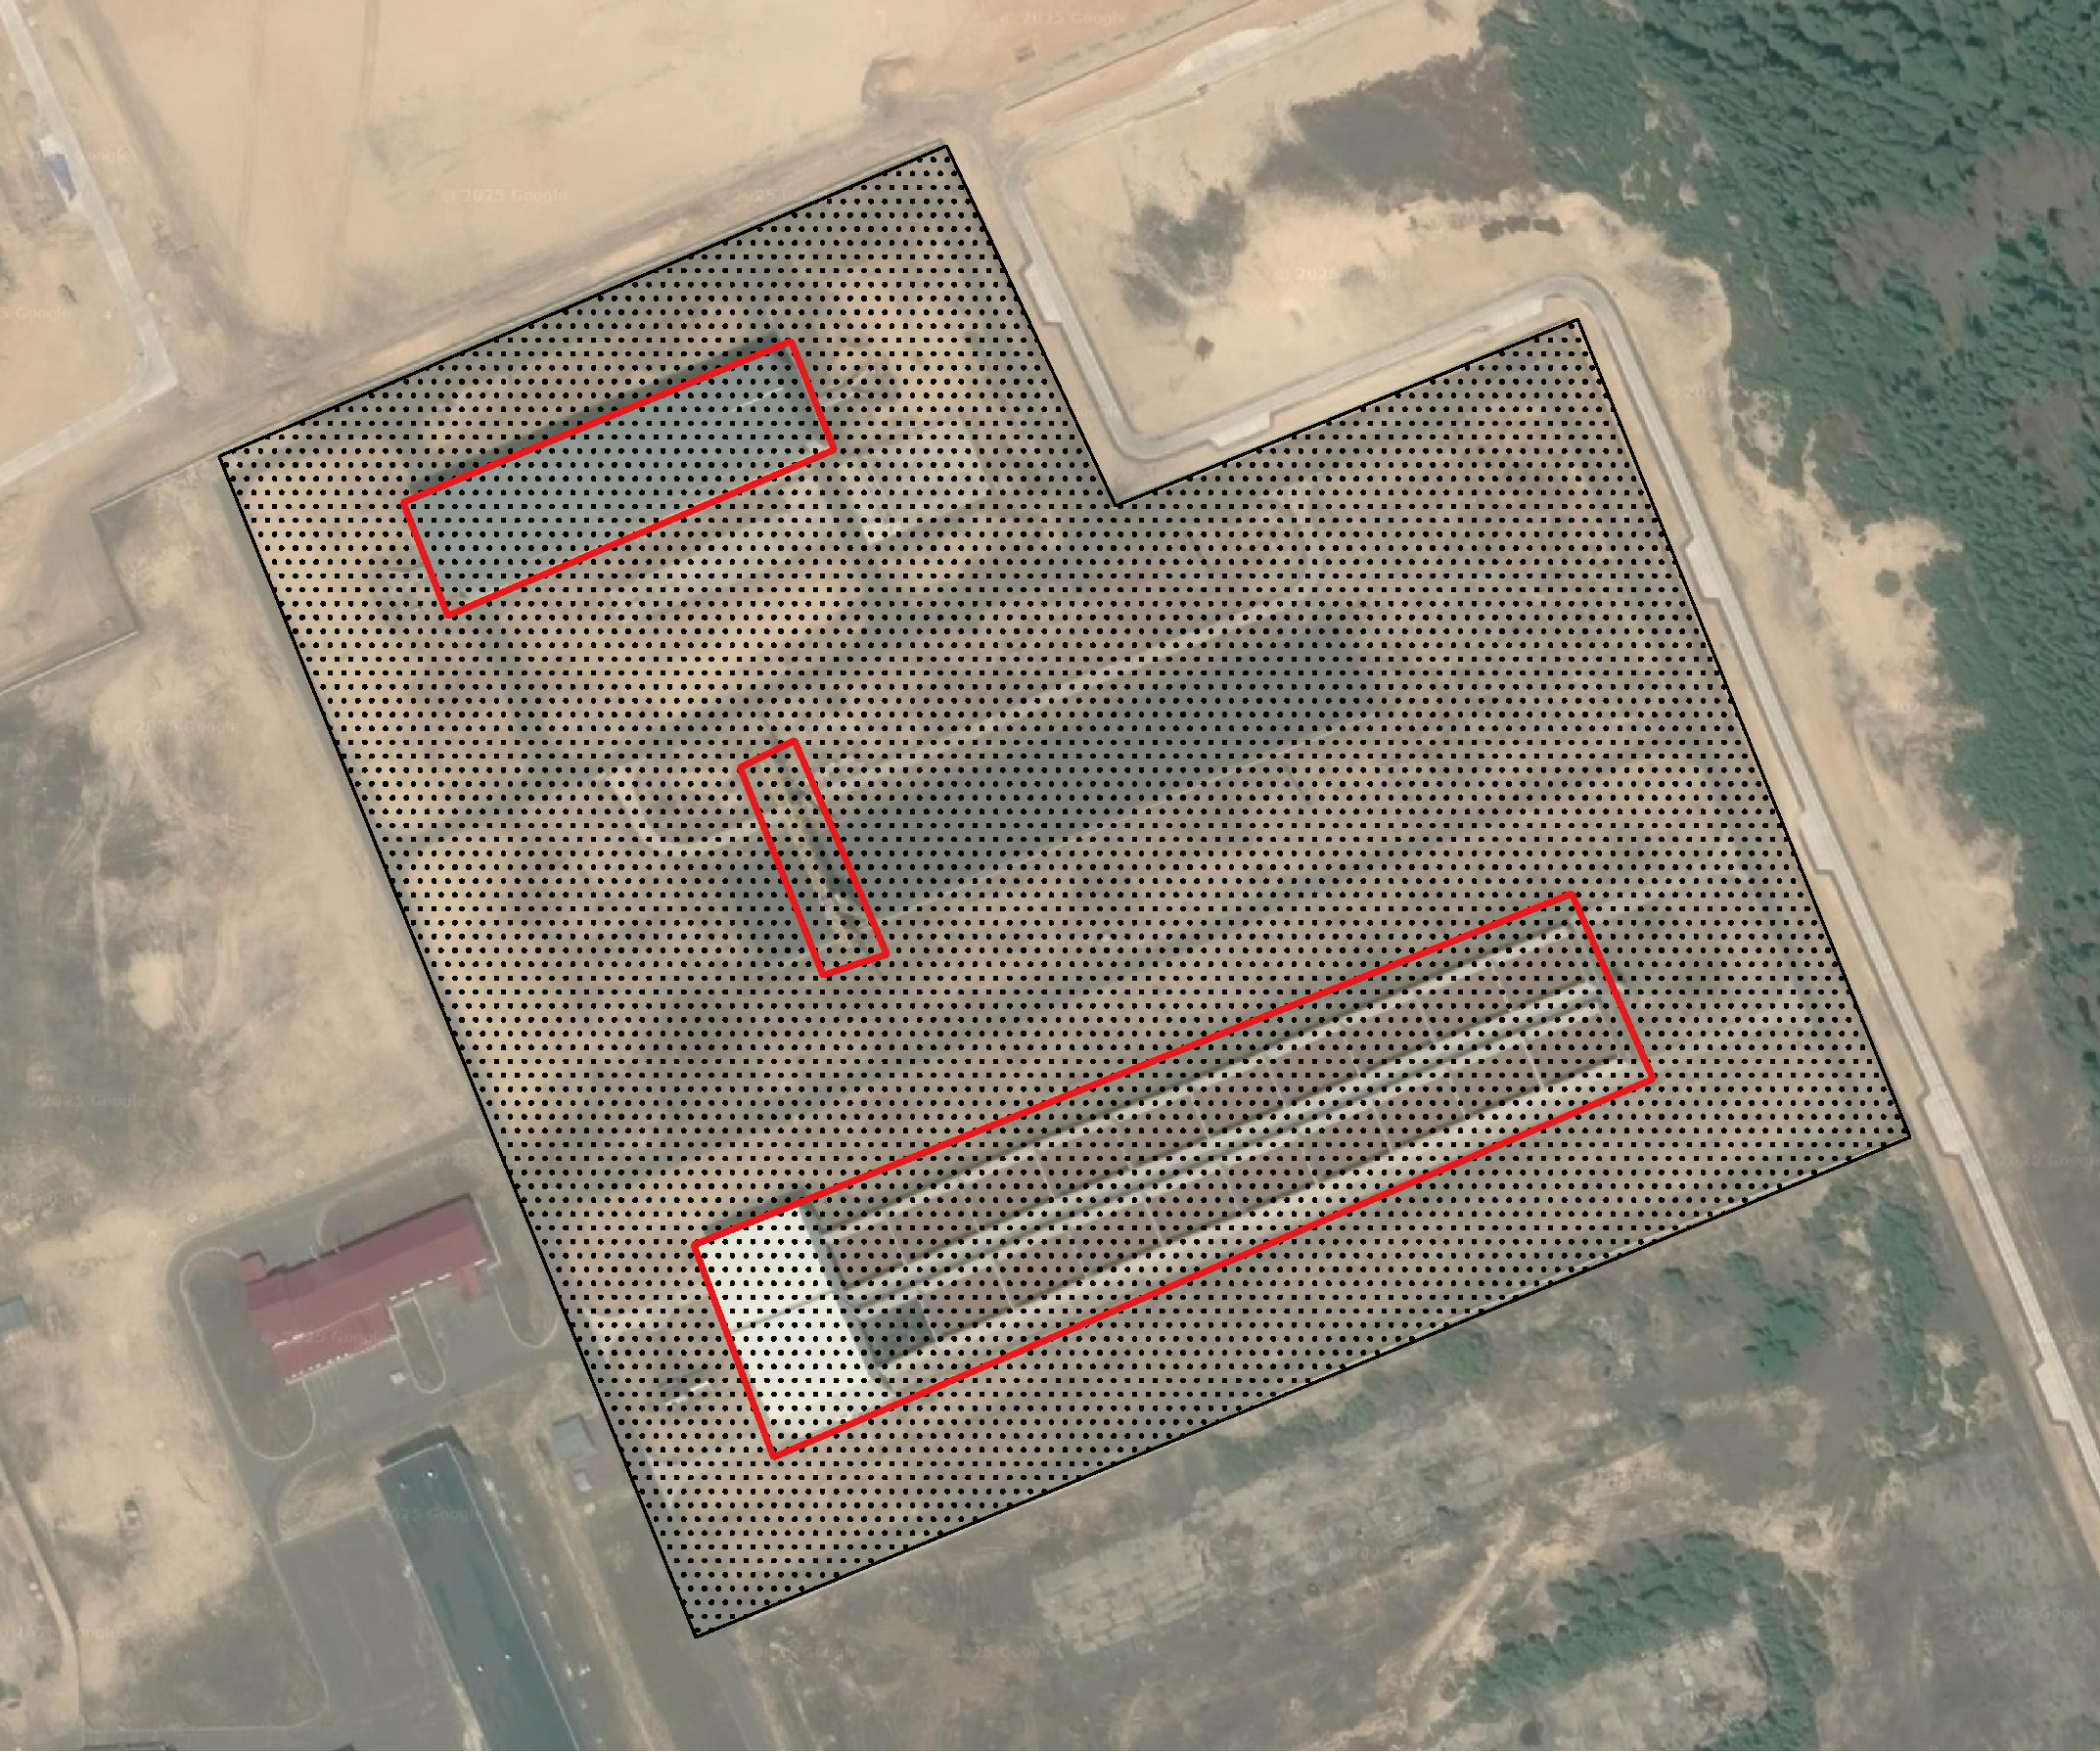
\includegraphics[width=0.45\textwidth]{figs/Jihwan/map2.pdf} \\
        (a) & (b) \\[10pt]
        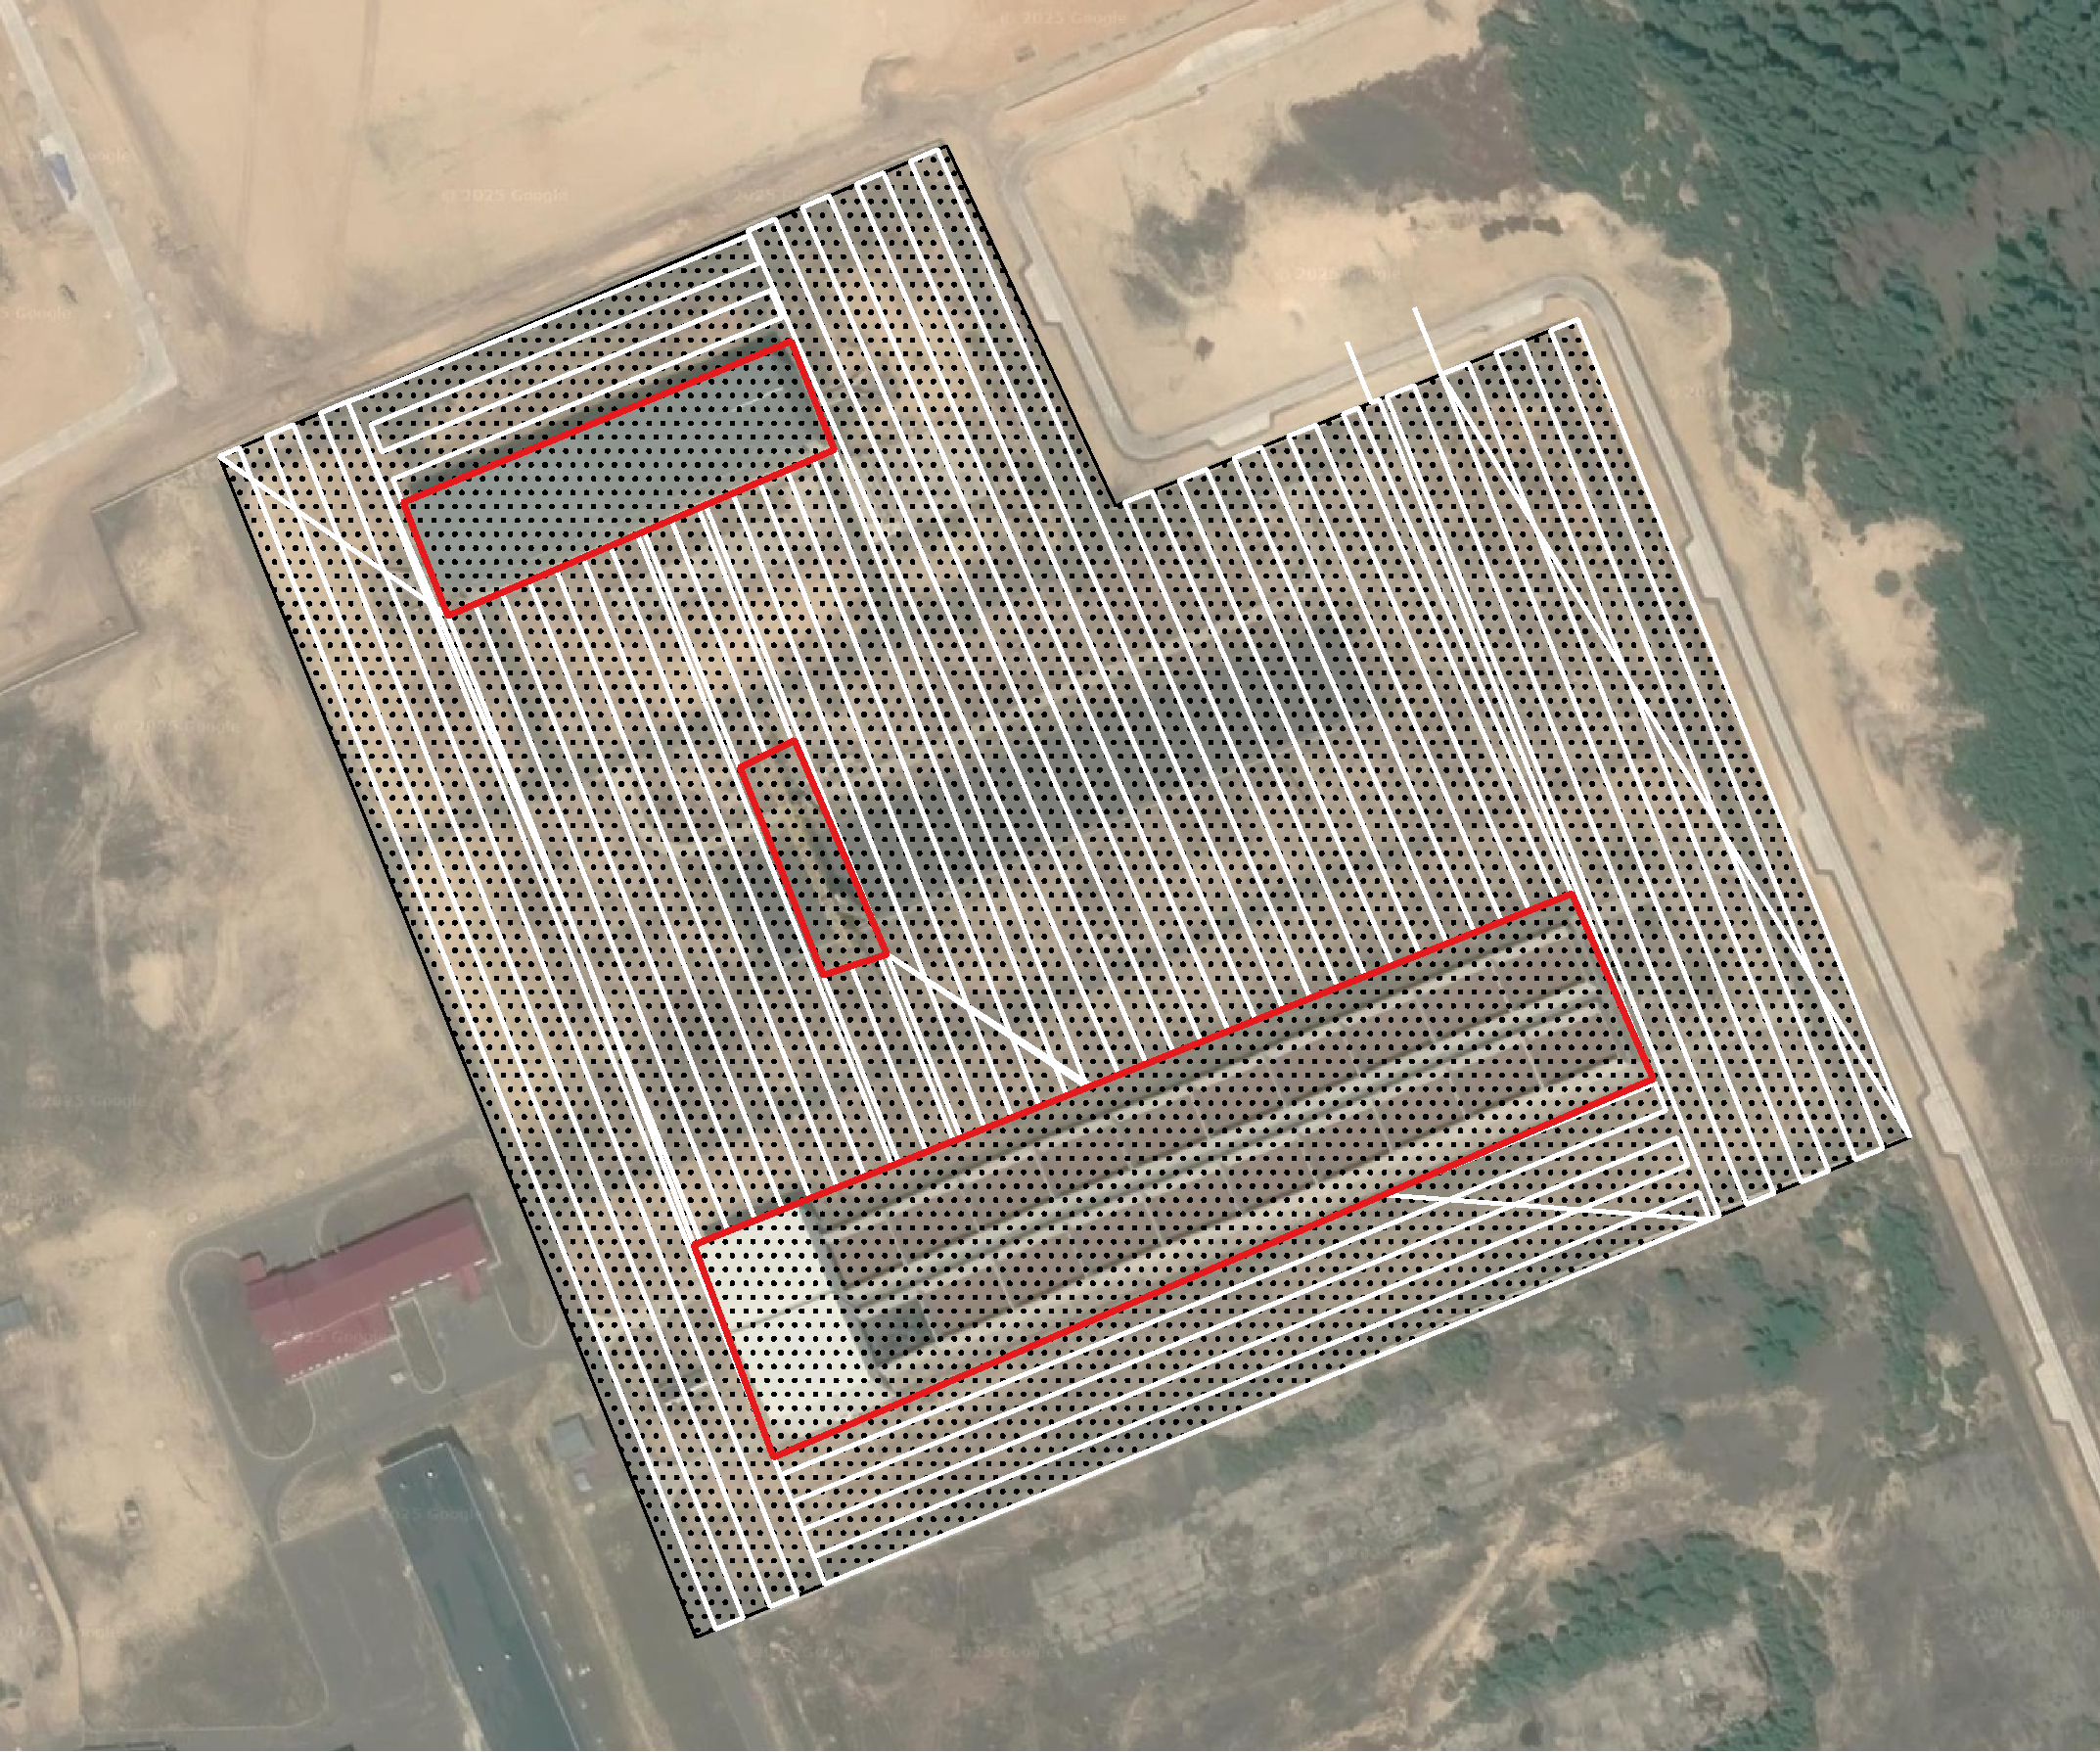
\includegraphics[width=0.45\textwidth]{figs/Jihwan/map3.pdf} &
        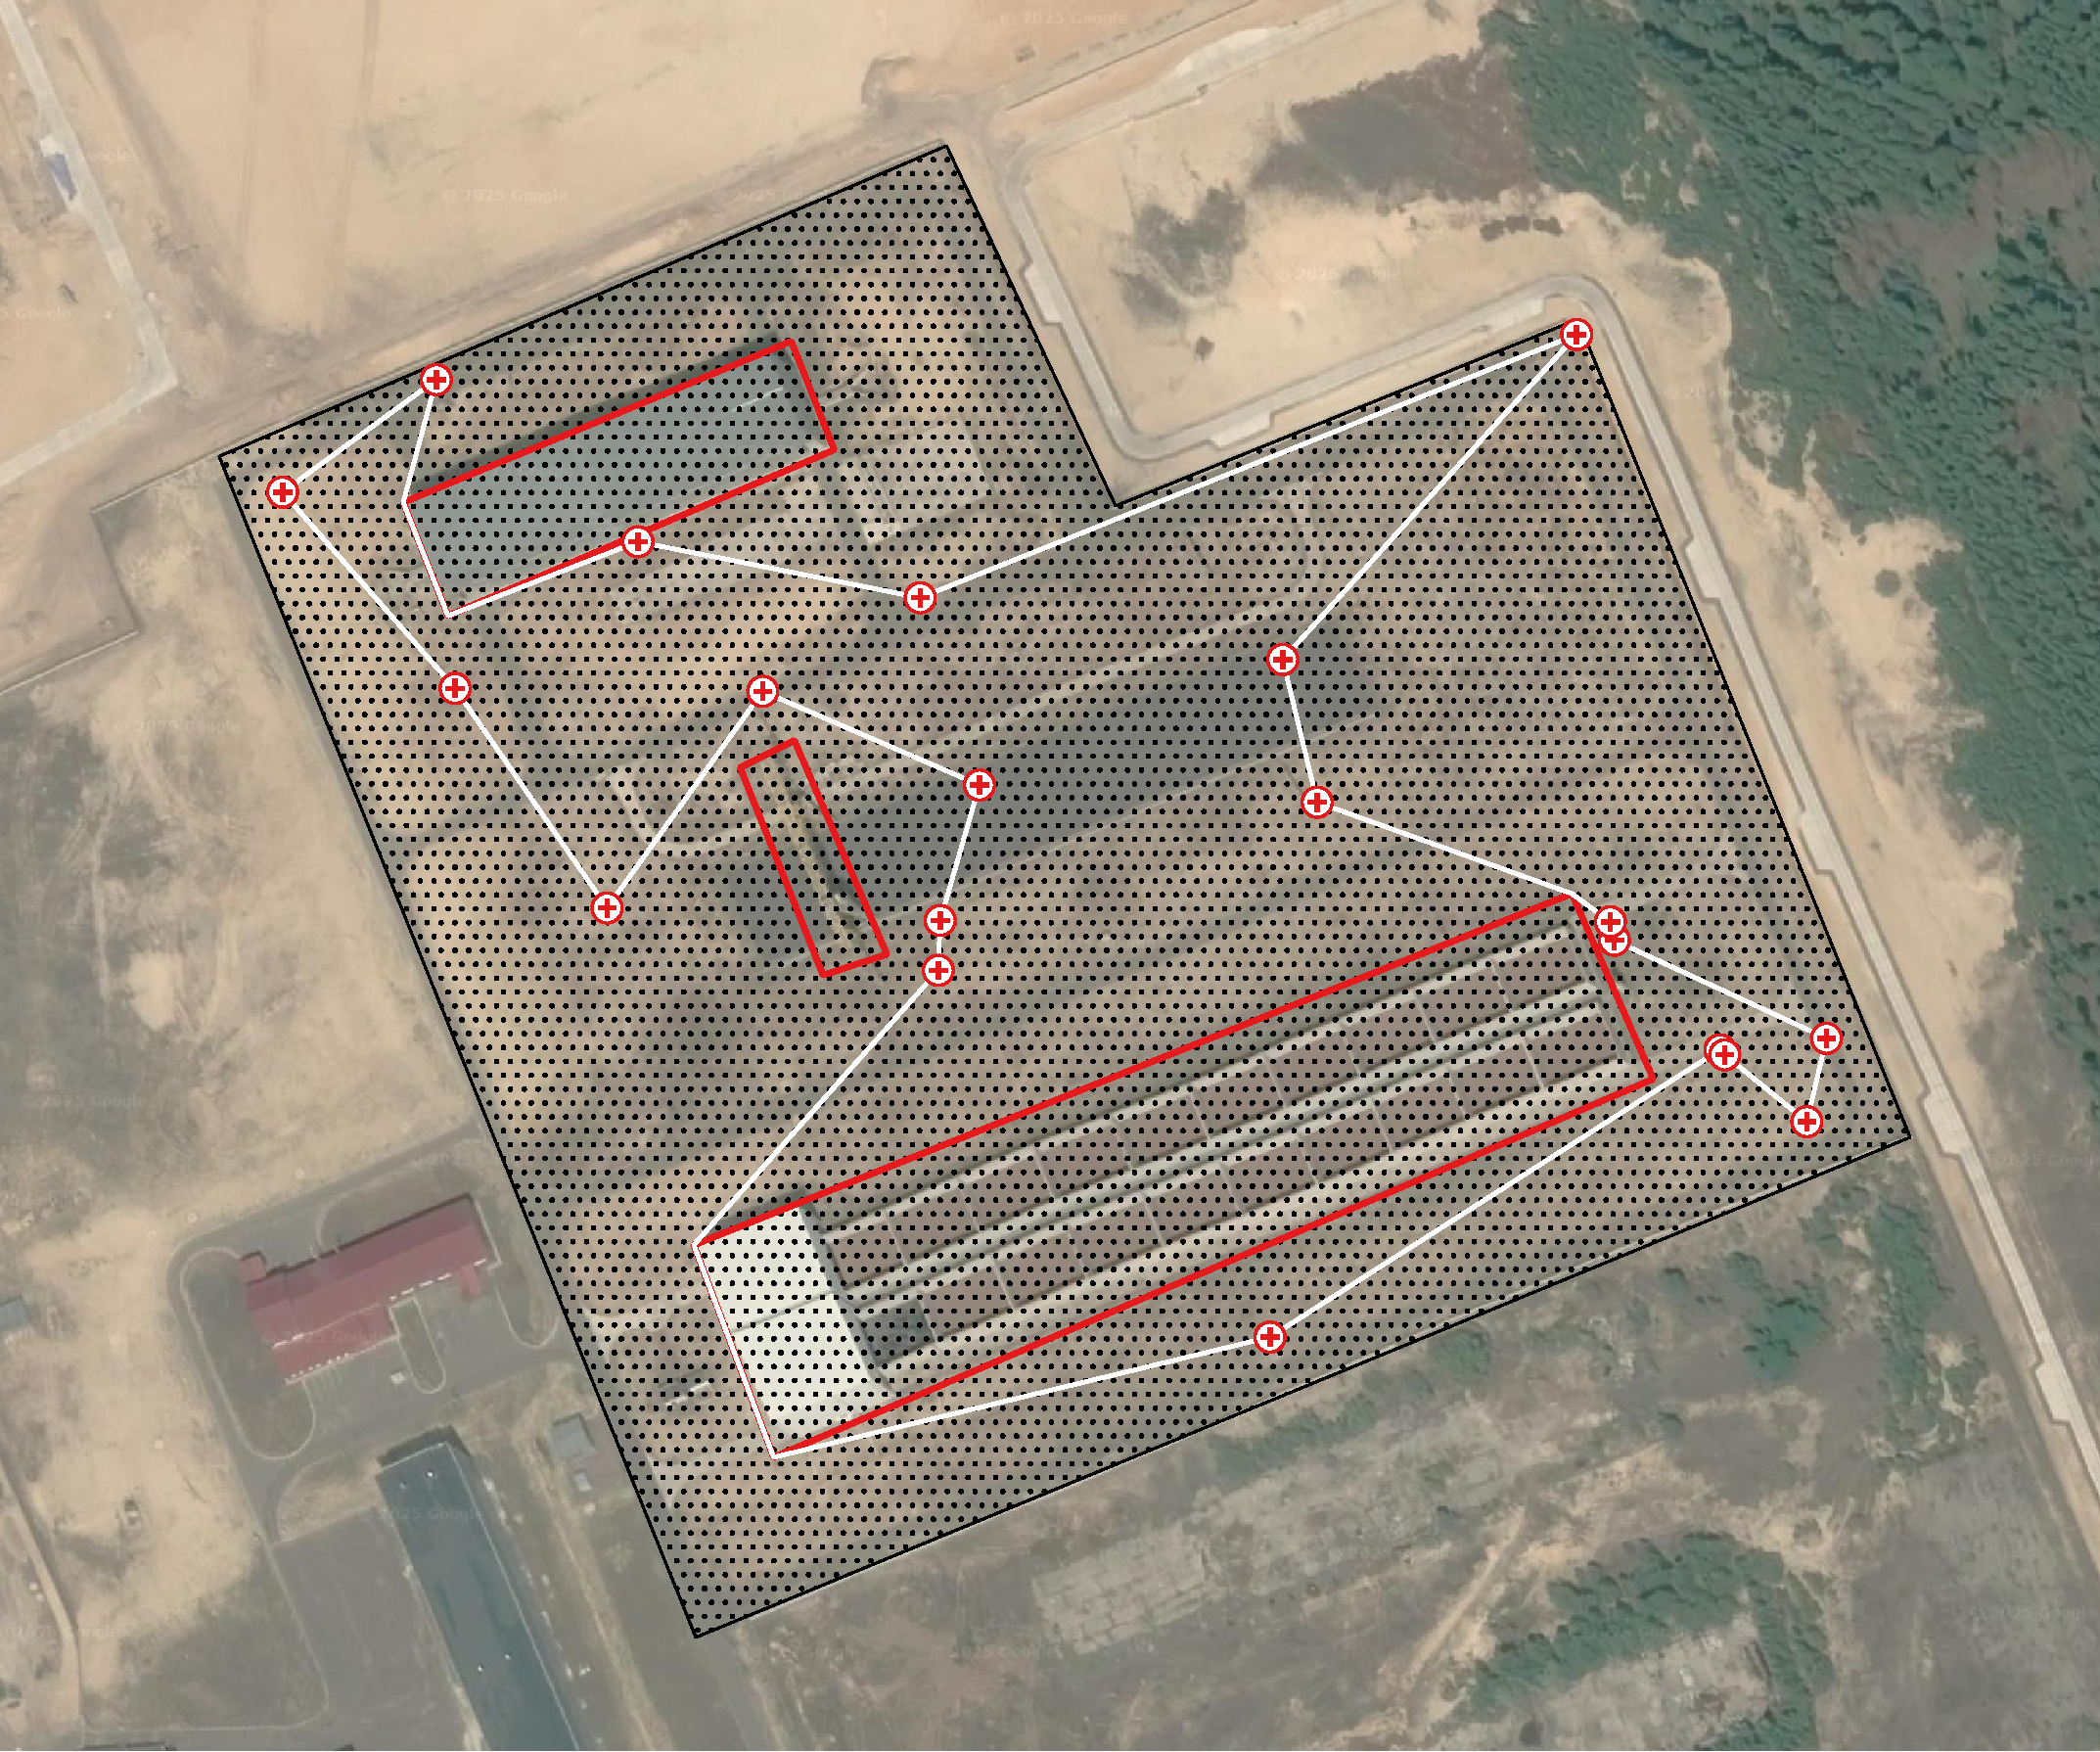
\includegraphics[width=0.45\textwidth]{figs/Jihwan/map4.pdf} \\
        (c) & (d)
    \end{tabular}
    \caption[Real Location Example for Mission Planning]
    {Real location example for generating a mission plan of a \gls{roi}. (a) The satellite view of a field in Ukraine. (b) The outer polygon (black dotted region) and holes (red regions) are drawn on \gls{qgis} to define the \gls{roi}. (c) The \gls{cpp} algorithm is executed to generate the thermal sensor drone path plan. (d) The \gls{tspo} algorithm is executed with 20 suspected landmine points to generate the \gls{GPR} sensor drone path plan. 
    }
    \label{fig:msp_example}
\end{figure}

%%%%%%%%%%
\subsection{Expanding to a Multi-Drone Operation}
\label{sec:msp_multi_drone}

Thus far, the mission planning algorithm has been explored for a single-drone operation. To make the system expandable, we must consider how to deploy a multi-drone system using the mission planning algorithm explained above. To do so, we introduce the Divide and Cluster method (based on \cite{skorobogatov2021multi}) for this problem. The method starts by dividing the \gls{roi} into smaller cells, which then get clustered into subregions that can be surveyed by individual drones adopting the layered approach.

\subsubsection{Divide and Cluster}

\paragraph{Divide} To divide the \gls{roi}, we can use triangulation algorithms which generate a mesh of triangles for a given set of vertices. In particular, we apply the \gls{cdt} from \gls{cgal} 2D Triangulations package \cite{cgal2024triangulation} to the \gls{roi}. Delaunay triangulation generates triangles which must conform to the Delaunay property: the circumcircle of a triangle must not include any other vertices than the triangle itself. \gls{cdt} is a variation in which pre-defined edges (i.e. the edges of the \gls{roi}) must be included in the final triangulation, while allowing some relaxation in the Delaunay property. The result of applying \gls{cdt} to an example Polygon with Holes is shown in Figure~\ref{fig:msp_cdt}. 

\begin{figure}[h!]
    \centering
    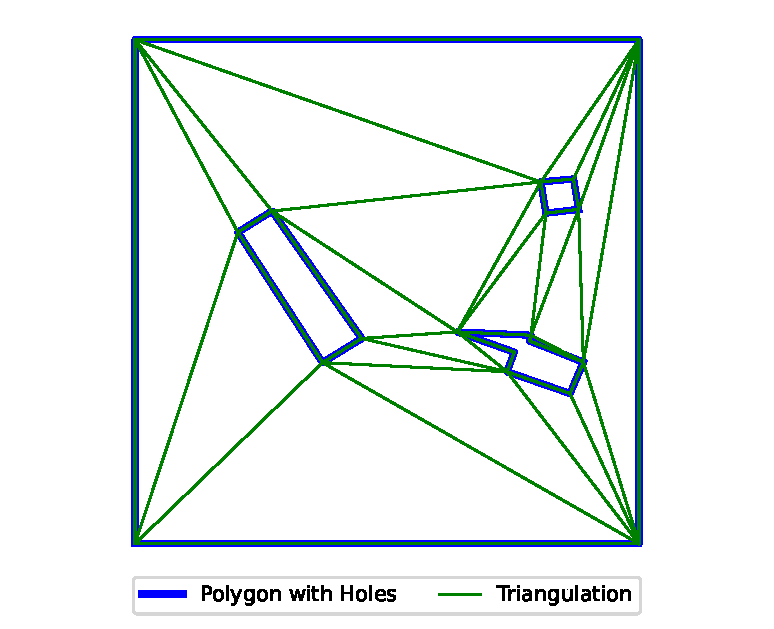
\includegraphics[width=0.6\linewidth]{figs/Jihwan/cdt.pdf}
    \caption[Constrained Delaunay Triangulation of Polygon with Holes]
    {The \gls{cdt} of a Polygon with Holes has been generated using \gls{cgal}'s 2D Triangulations package.}
    \label{fig:msp_cdt}
\end{figure}

\paragraph{Cluster} The divided mesh should now be clustered to form $n$ subregions that are each covered by a drone. The resulting subregions should meet 2 requirements: high compactness ($\mathrm{Compactness} = \frac{\mathrm{Area}}{\mathrm{Perimeter}}$ is maximised to generate a more efficient \gls{bcd} path) and similarity in area (so that each drone gets a fair share which allows us to deploy the least number of drones). Possible options for the clustering algorithm include methods based on region-growing (seed triangles are allocated and grow into adjacent triangles until $n$ subregions remain, similarly to \cite{skorobogatov2021multi}) and METIS \cite{karypis1997metis} (multi-level graph partitioning algorithm can be applied on the mesh), which need to be implemented and tested for validation. 

The Divide and Cluster method is visualised by Figure~\ref{fig:msp_divide_cluster} where the clusters have been manually allocated to demonstrate the idea in theory. A real implementation of the clustering algorithm will need to be made to fully validate the method in practice. 

\begin{figure}[h!]
    \centering
    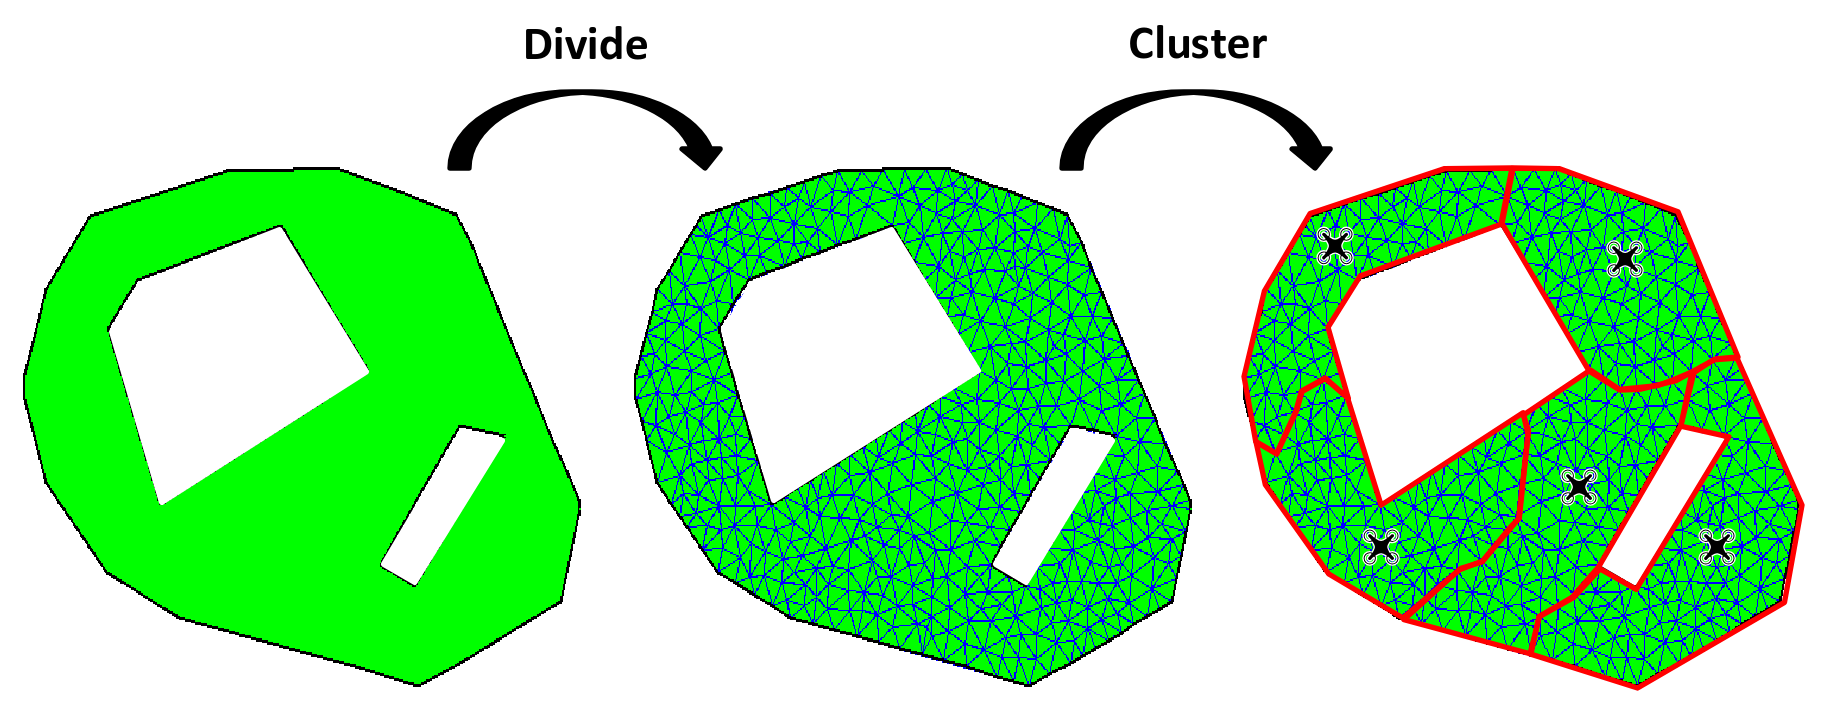
\includegraphics[width=\linewidth]{figs/Jihwan/Divide and Cluster.png}
    \caption[Divide and Cluster Method]
    {Divide and Cluster method visualised. A Polygon with Holes is divided using constrained Delaunay triangulation, then clustered into 5 subregions which can each be covered by a drone adopting the layered approach. The Polygon with Holes and the triangulation have been adopted from an example by \cite{cgal2024triangulation}.}
    \label{fig:msp_divide_cluster}
\end{figure}

\subsubsection{Possible Alternatives and Improvements}

\paragraph{Line Division} Instead of the Divide and Cluster method, the \gls{roi} may be directly decomposed into $n$ subregions of equal area using $n-1$ parallel line segments. This offers algorithm simplicity and greatly reduced computation times, but it is more likely to generate inefficient coverage paths as the compactness requirement is not considered. 

\paragraph{Boustrophedon Division} \gls{bcd} algorithm could be used during the Divide stage instead of \gls{cdt}, which would result in more appropriate polygons for generating boustrophedon coverage paths. However, \gls{bcd} tends to generate a smaller number of cells than \gls{cdt} which may make it harder to achieve the compactness and area requirements.  

\paragraph{Constrained Conforming Delaunay Triangulation} The example of \gls{cdt} in Figure~\ref{fig:msp_cdt} shows irregularly shaped and sized triangles being formed, which makes it harder to achieve the compactness and area requirements. \cite{shewchuk1996triangle} provides an implementation of the \gls{ccdt} which can be used to generate a more ideal mesh as demonstrated in Figure~\ref{fig:msp_shewchuk}. Additional software will need to be written to apply the algorithm to our \gls{cgal} Polygon with Holes object. 

\begin{figure}[h!]
    \centering
    \begin{tabular}{p{0.3\textwidth}p{0.3\textwidth}p{0.3\textwidth}}
        
\includegraphics[width=0.3\textwidth]{figs/Jihwan/triangulation_original.png} &
        
\includegraphics[width=0.3\textwidth]{figs/Jihwan/triangulation_cdt.png} &
        
\includegraphics[width=0.3\textwidth]{figs/Jihwan/triangulation_ccdt.png} \\
        \centering (a) The letter A (\gls{roi}). & 
        \centering (b) After applying \gls{cdt}. & 
        \centering (c) After applying \gls{ccdt}.
    \end{tabular}
    \caption[Comparison of Triangulation Methods]
    {Comparison of \gls{cdt} and \gls{ccdt} applied to the letter A, taken from \cite{shewchuk1996triangle}.}
    \label{fig:msp_shewchuk}
\end{figure}


%%%%%%%%%%
\subsection{Comparison with Previous Landmine Detection Systems}
\label{sec:msp_comparison_manual_demining}

\subsubsection{Efficiency}

To evaluate the efficiency of the landmine detection system, we can compare the coverage time per unit area ($\varepsilon$). The expressions for the layered, magnetic-sensor (a commonly used option for aerial landmine detection systems) and manual approaches are shown in Equations \ref{eq:msp_layeredefficiency}, \ref{eq:msp_magneticefficiency} and \ref{eq:msp_manualefficiency} respectively using symbols explained in Table \ref{tab:msp_efficiencyvariables}.
\begin{equation}
\label{eq:msp_layeredefficiency}
\varepsilon_{\mathrm{layered}} = \frac{\frac{C_{\mathrm{thermal}}}{v_{\mathrm{thermal}}}+\frac{T_{\mathrm{GPR}}}{v_{\mathrm{GPR}}}+n_{\mathrm{suspected}} \times t_{\mathrm{GPR}}}{A_{\mathrm{ROI}}}
\end{equation}
\begin{equation}
\label{eq:msp_magneticefficiency}
\varepsilon_{\mathrm{magnetic}} = \frac{\frac{C_{\mathrm{magnetic}}}{v_{\mathrm{magnetic}}}}{A_{\mathrm{ROI}}}
\end{equation}
\begin{equation}
\label{eq:msp_manualefficiency}
\varepsilon_{\mathrm{manual}} = \frac{t_{\mathrm{manual}}}{A_{\mathrm{ROI}}}
\end{equation}

\begin{table}[h!]
    \centering
    \begin{tabular}{|c|p{0.5\linewidth}|c|}
    \hline
        \textbf{Symbol} & \textbf{Explanation} & \textbf{Unit} \\
    \hline\hline
        $\varepsilon_{\mathrm{method}}$ & Coverage time per unit area of the given method. & $\mathrm{m}^{-2} \cdot \mathrm{s}$ \\
    \hline
        $C_{\mathrm{sensor}}$ & Length of the coverage path generated using \gls{bcd} algorithm for the coverage width of the given sensor.  & $\mathrm{m}$ \\
    \hline
        $v_{\mathrm{sensor}}$ & Maximum flight speed of the drone attached with the given sensor. & $\mathrm{m} \cdot \mathrm{s}^{-1}$ \\
    \hline
        $T_{\mathrm{GPR}}$ & Length of the target path generated using \gls{tspo} algorithm that should be surveyed using the \gls{GPR} sensor. & $\mathrm{m}$ \\
    \hline
        $n_{\mathrm{suspected}}$ & Number of suspected landmine points that must be visited by the \gls{GPR} sensor. & N/A \\
    \hline
        $t_{\mathrm{GPR}}$ & The fixed time required to perform the scanning procedure for a point of interest using the \gls{GPR} sensor as described in Section \ref{GPR_flight} & $\mathrm{s}$ \\
    \hline
        $t_{\mathrm{manual}}$ & Time taken for the \gls{roi} to be fully covered using manual detection methods. & $\mathrm{s}$ \\
    \hline
        $A_{\mathrm{ROI}}$ & Area of the \gls{roi}. & $\mathrm{m}^{2}$ \\
    \hline
    \end{tabular}
    \caption[Explanation of Variables for Mission Efficiency Expressions]
    {Explanation of the variables used in Equations \ref{eq:msp_layeredefficiency}, \ref{eq:msp_magneticefficiency} and \ref{eq:msp_manualefficiency} to express the mission efficiency.}
    \label{tab:msp_efficiencyvariables}
\end{table}

It is difficult to quantify an exact value for the improvement in efficiency by adopting the layered approach because the values of $C_{\mathrm{sensor}}$, $v_{\mathrm{sensor}}$ and $T_{\mathrm{GPR}}$ are dependent on the specifications of the chosen sensors, geometry of the \gls{roi} and the density of the suspected landmine points. 

For the manual method, \cite{gichd2005manual} provides a value of 12.5 to 125\,m$^2$ per deminer per day. This is a large range which varies depending on the quality of the workers and management.

The coverage width of a magnetic sensor is suggested to be 1\,m according to \cite{Yoo2024UnmannedAV} compared to 9\,m of our chosen thermal sensor, which would result in a significantly longer $C_{\mathrm{sensor}}$ (similarly to Figure~\ref{fig:msp_bahnemann}). The main argument for improvement in efficiency of the layered approach comes from the decision to use a thermal sensor during the Cover step which is significantly faster than its alternatives. However, most of the remaining parameters could not be found in related works on thermal, \gls{GPR} and magnetic sensor equipped drones as they vary depending on the specification and fine-tuning. For a credible comparison, real world experiments need to be conducted for various geometries of \gls{roi} and levels of landmine density.  

\subsubsection{Expandability}

In manual mine detection systems, additional human resources should be added to cover a larger area of land which is both costly and difficult to obtain. The proposed mission planning framework greatly improves the expandability by utilising the multi-aerial drone system with the Divide and Cluster method, allowing the operator to survey larger areas by deploying additional drones and base stations. 

\subsubsection{Intuitiveness}

The layered approach offers an intuitive solution by incorporating the \gls{qgis} interface and automatic path planning algorithms which can be used even by inexperienced operators in demining organisations. The system also returns the analysed data in a more interpretable format through \gls{qgis} maps, which helps the demining organisations plan future missions more efficiently.

%%%%%%%%%%
\subsection{Limitations}
\label{sec:msp_limitations}

To further improve the mission planning framework, some of its limitations are listed below along with suggestions on how they can be mitigated. 

\subsubsection{Manually Labelled Region of Interest}

In the Define step of the layered approach, the operator must manually label the outer boundary and obstacles of the \gls{roi} using the polygon tool in \gls{qgis}. This becomes a time-consuming task as more vertices are introduced, and the manual procedure also introduces an inconsistency in the definition of the \gls{roi}. If multiple operators work on defining the obstacles in a large \gls{roi}, the offset required for safe maneuver by the drones may differ. 

As a solution, image segmentation algorithms can be implemented to partially automate this process. Image segmentation models like Segment Anything Model 2 \cite{ravi2024sam2} can be used to automatically identify the vertices of obstacles which can be selected and adjusted by the operator. 

\cite{patil2022segment} proposes a more specialised semantic segmentation model to automatically segment satellite images into regions and identify its class (building, land, road, vegetation, water, or miscellaneous). This can speed up the progress of defining the \gls{roi} by removing areas such as bodies of water and buildings which are unlikely to be populated by landmines. 

\subsubsection{Use of Satellite Image Databases}
\label{sec:msp_satellite_database_limitation}

The current mission planning framework uses openly available satellite databases during the Define step of the layered approach. However, outdated satellite images may result in missing out newly introduced or removed obstacles in the \gls{roi}. 

Mine Kafon\footnote{\url{https://minekafon.org/}} deploys a lightweight mapping drone (MK Destiny) to automatically generate the 3D map of the \gls{roi}. The \gls{cpp} algorithm could be modified to deploy a drone equipped with RGB camera to map the \gls{roi} in a similar way.  

\subsubsection{Streamlining the User Interface}

The \gls{cpp} and \gls{tspo} algorithms are not directly connected to the \gls{qgis} interface; currently, the user must manually import and export the \gls{roi} and path plans as a GeoJSON format before and after running the C++ scripts. 

\gls{qgis} allows developers to create custom Python plugins to add additional functionalities to the interface. By wrapping the \gls{cpp} and \gls{tspo} algorithms \gls{qgis} plugins, the operator will be able to easily run these algorithms within the interface without having to compile or run C++ scripts on their own. 

\subsubsection{Testing in Real World Scenarios}

In this report, the mission planning framework was tested for a real location example in Figure~\ref{fig:msp_example}. However, the example does not fully demonstrate a real multi-aerial drone system using the Divide and Cluster method.

Real world testing will need to be conducted for a variety of different \gls{roi} locations (with varying terrains, soil composition, weather conditions, etc.), evaluating the efficiency of the proposed mission planning framework. This will help to create a robust system that can easily be applied across different regions and scenarios. 
\newpage
\fancyhead[C]{Jihwan Shin}
\section{Extra-UAV Communication Architecture} \label{sec:extra_uav_communication}

%%%%%%%%%%
\subsection{System Requirements}
\label{sec:euc_requirements}

- explain the concept of a base station
- outline what extra uav communication we need
- calculate the bit rate requirement for our information as a variable expression
- requirement to fly in various regions, laws on communication frequency

\subsubsection{Base Station}
- what is processed in the base station
- located near the roi
- explain necessity with comms with the base station during mission 

\subsubsection{Extra-UAV Communication Content}
- gnss, return to safety, return to home, etc.
- how many drones and how frequently
- resulting bit rate requirement


\begin{table}
    \centering
    \begin{tabular}{|c|c|c|}
        \hline Data & Detail & Bits \\
        \hline 
        \hline Drone ID & Distinct ID for each drone & 8 \\
        \hline Return to Safety & Boolean value & 1 \\
        \hline 
        \hline \multicolumn{2}{|c|}{Total} & 000 \\
        \hline 
    \end{tabular}
    \caption{Caption}
    \label{tab:my_label}
\end{table}

\subsubsection{Technical Requirements}
- distance
- bitrate (explained above)
- geographical region
- legality

\subsection{LoRa Communication}
\label{sec:euc_lora}

\subsubsection{LoRa and LoRaWAN Theory}

- phy, mmac, sf, etc. 

\subsubsection{Advantages}

\paragraph{Power Consumption}

\paragraph{Distance}

\paragraph{Costs}

\subsubsection{Disadvantages}

\paragraph{Bit-rate}

\paragraph{Bandwidth}

\subsection{Example Simulation}
\label{sec:euc_example_sim}

\subsubsection{ns-3}

\paragraph{LoRaWAN Module}

\paragraph{Mobility Module}

\subsubsection{Scenario}

\subsubsection{Results}

\subsubsection{Integration with the Mission Planning Framework}


\newpage
\pagenumbering{arabic}
\fancyhead[C]{Huirui Dai}
\section{Hardware} \label{hardware}
\newpage
\fancyhead[C]{Huirui Dai}
\setlength{\parindent}{0pt}

\section{Data Acquisition} \label{data acquisition}

\subsection{Landmines}

The selection of sensing hardware in our multi-drone landmine detection system relies on a clear understanding of the target: landmines. Landmines differ widely in size, materials, triggering mechanisms, and intended targets. These physical differences strongly affect how detectable they are, especially when using drones with limited payload capacity. This section outlines the main landmine types and highlights the features that influence detection. This overview supports informed decisions on sensor selection and data acquisition in our system.

Landmines are commonly classified into two main categories based on their intended targets: anti-tank landmines (ATLs) and anti-personnel landmines (APLs).
\footnote{\url{https://en.wikipedia.org/wiki/Land_mine}}

ATLs are designed to disable or destroy heavy vehicles such as tanks or armored transports. They are typically large, with diameters ranging from 13 to 40 cm, and contain 6 to 11 kg of explosives\cite{paik2002image}. These mines are generally triggered by high pressures and are often buried beneath roadways or terrain. Traditional ATLs use metal casings, but modern designs may incorporate plastic or composite materials to reduce detectability \cite{evans2024detection}. Based on their activation mechanisms, ATLs can be classified into pressure-activated blast mines, tilt-rod or magnetic mines, and side-attack mines.

APLs are intended to injure or kill individuals on foot. They are much smaller than ATLs, typically ranging from 6 to 15 cm in diameter, and contain only 0.1 to 4 kg of explosives\cite{paik2002image}. These mines are triggered by very low pressure, often below 10 kg, which makes them highly dangerous and difficult to detect. APLs are commonly constructed from plastic, rubber, or other low-metal-content materials, further reducing their detectability \cite{kaya2017buried}. Like ATLs, APLs are also divided into subtypes, including blasting mines, bounding fragmentation mines, and directional fragmentation mines.

\begin{figure}[h]
    \centering
    \begin{subfigure}[b]{0.24\textwidth}
        \centering
        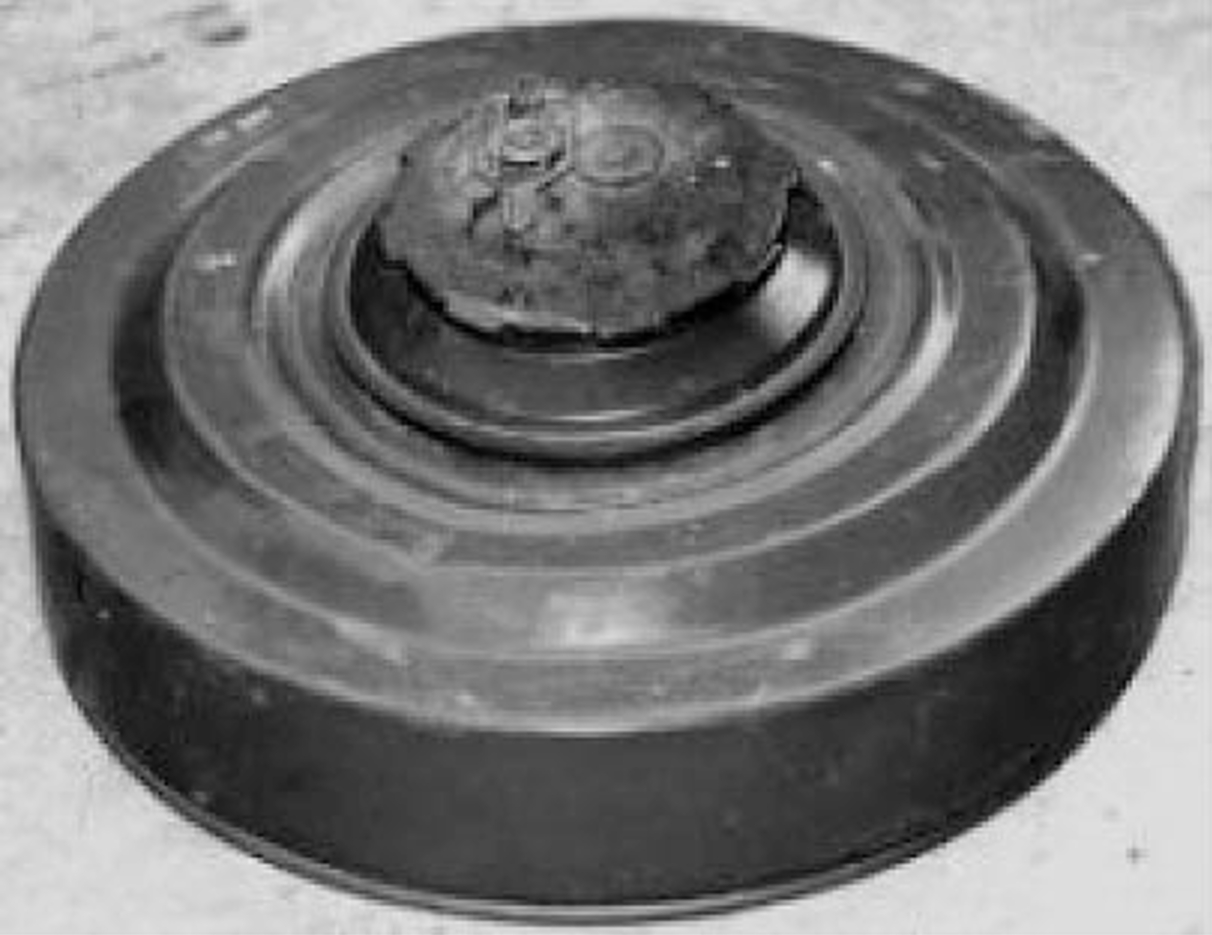
\includegraphics[height=2cm]{figs/Huirui/tm62m.png}
        \subcaption*{(a)}
    \end{subfigure}
    \begin{subfigure}[b]{0.24\textwidth}
        \centering
        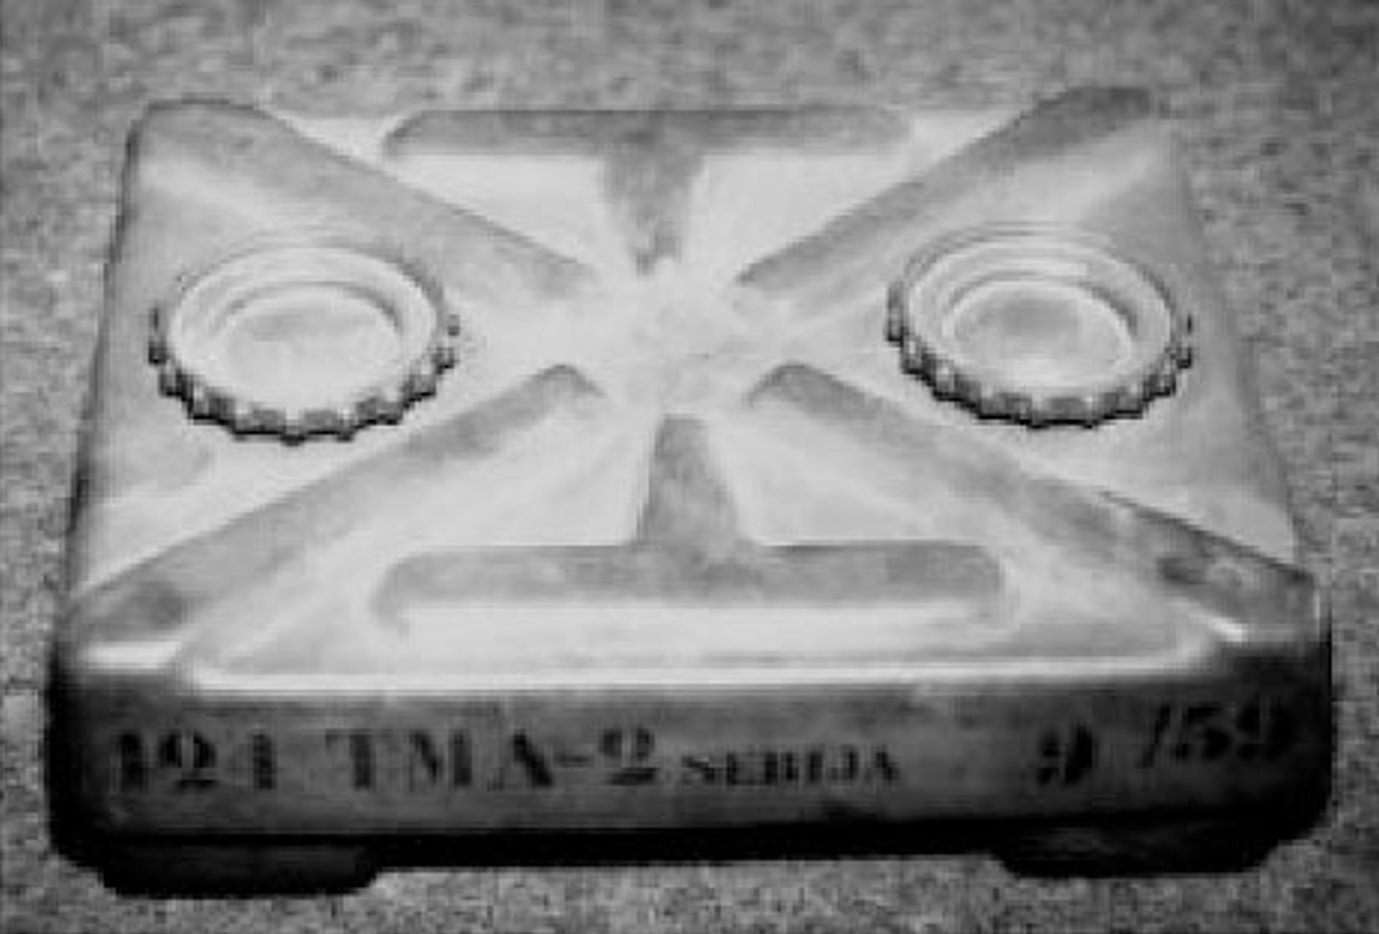
\includegraphics[height=2cm]{figs/Huirui/tma2.png}
        \subcaption*{(b)}
    \end{subfigure}
    \begin{subfigure}[b]{0.24\textwidth}
        \centering
        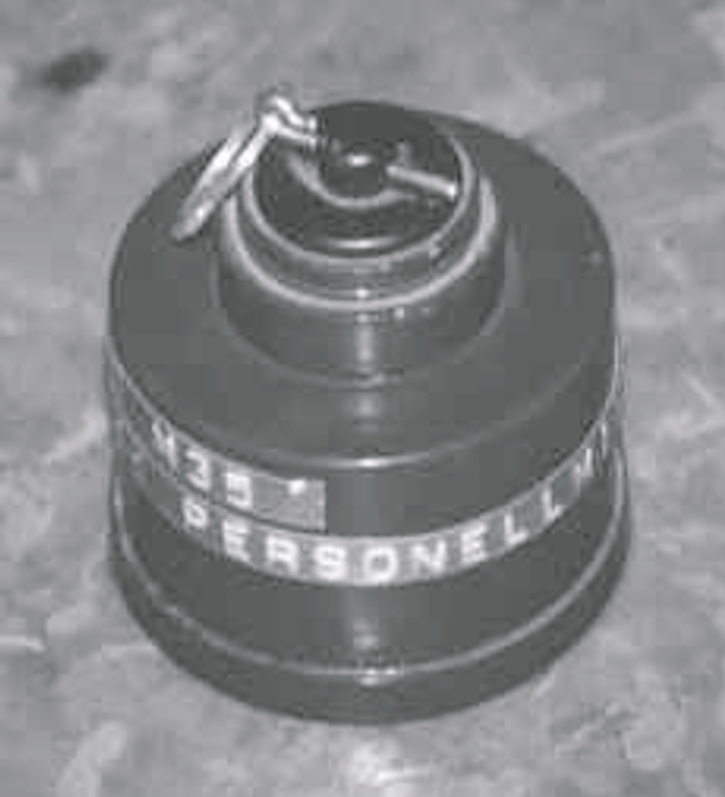
\includegraphics[height=2cm]{figs/Huirui/prbm35.png}
        \subcaption*{(c)}
    \end{subfigure}
    \begin{subfigure}[b]{0.24\textwidth}
        \centering
        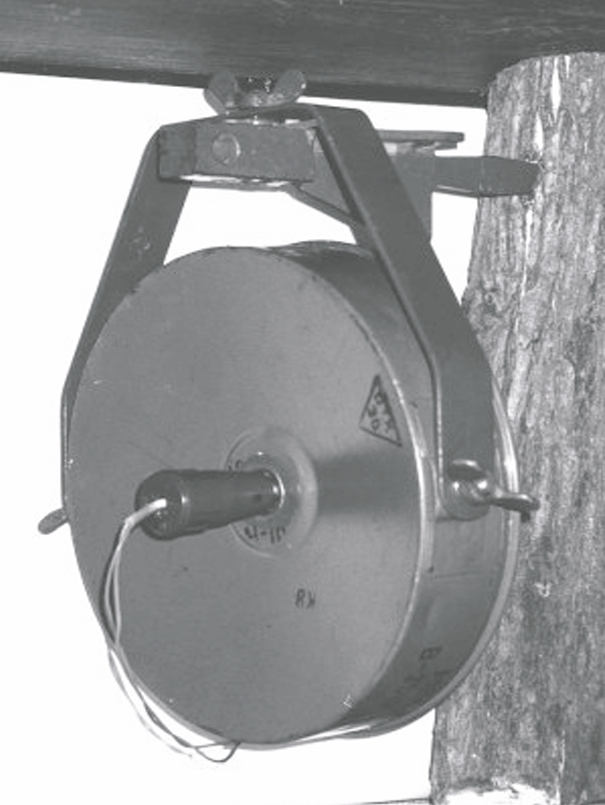
\includegraphics[height=2cm]{figs/Huirui/mon100.png}
        \subcaption*{(d)}
    \end{subfigure}

    \caption{Typical ATLs and APLs: (a) TM-62M, (b) TMA-2, (c) PRB-M35, and (d) MON-100~\cite{paik2002image}.}
    \label{fig:mine_examples}
\end{figure}


\begin{table}[h]
    \centering
    \small
    \renewcommand{\arraystretch}{1.3}
    \caption{Specifications for selected ATLs and APLs~\cite{paik2002image}.}
    \label{tab:mine_specs}
    \begin{tabular}{l p{2.8cm} p{2.8cm} p{2.8cm} p{2.8cm}}
        \toprule
        \textbf{Model No.} & \textbf{TM-62M} & \textbf{TMA-2} & \textbf{PRB-M35} & \textbf{MON-100} \\
        \midrule
        Type & ATL & ATL & APL & APL \\
        Height (cm) & 11.2 & 14.0 & 5.7 & 8.2 \\
        Diameter / Width (cm) & 31.6 & 26.0 × 20.0 & 6.4 & 23.6 \\
        Weight (kg) & 8.5 & 7.5 & 0.16 & 5.0 \\
        Material & Steel & Plastic & Plastic & Steel \\
        Sensitivity & 200 kg & 120 kg & 8 kg & Depends on fuses \\
        \bottomrule
    \end{tabular}
\end{table}

Figure~\ref{fig:mine_examples} shows four representative examples of ATLs and APLs, and Table~\ref{tab:mine_specs} summarizes their key structural specifications. As the table indicates, both ATLs and APLs can be constructed from metallic, low-metallic, or non-metallic materials. However, APLs are significantly smaller in size, which make them more difficult to detect, especially from aerial platforms. And from a technical perspective, a system capable of reliably detecting small APLs is also likely to detect the larger ATLs. Also, nowadays APLs are more responsible for the vast majority of civilian injuries and deaths in post-conflict areas compared with ATLs \cite{unmas2021handbook}, which underscores their humanitarian significance. For these reasons, our project focuses on the detection of anti-personnel landmines.

\subsection{Sensors}

\subsubsection{Landmine Detection Techniques}

Landmine detection technologies have evolved to encompass a wide range of sensing principles, each targeting specific physical, chemical, or biological characteristics of surface-laid and buried mines. Broadly, these methods can be categorized into five general classes: \textit{\textbf{electromagnetic induction-based} techniques}, \textit{\textbf{radiowave and microwave-based} systems}, \textit{\textbf{mechanical and vibro-acoustic} methods}, \textit{\textbf{spectral and thermal imaging} approaches}, and \textit{\textbf{chemical and biological} sensing methods}. Within each class, a variety of specialized detection technologies have been developed, including traditional metal detectors, ground-penetrating radar, infrared and hyperspectral imaging, seismic/acoustic sensors, vapor detection, and biosensors. Each of these approaches offers distinct advantages and faces specific limitations, especially when adapted to drone-based platforms for remote and efficient minefield scanning. In the following subsections, each class is explored in detail, with emphasis on the operating principles, detection capabilities, challenges, and documented UAV-based applications.

\paragraph{Electromagnetic Induction-Based Techniques}

Electromagnetic induction (EMI) methods operate by exploiting the interaction between electromagnetic fields and conductive or magnetic materials in the ground. These systems are typically composed of a transmitter coil that emits a time-varying electromagnetic field into the soil. When this field encounters a conductive object—such as a landmine with metallic components—it induces eddy currents within the object, which in turn generate a secondary magnetic field. This field is detected by a receiver coil, and the resulting signal is processed to infer the presence of the object. These principles form the basis of conventional \textbf{metal detectors}~\cite{gichd2006guidebook}.

In contrast, \textbf{magnetic sensors} or magnetometers do not actively induce eddy currents but instead measure disturbances in the Earth's ambient magnetic field caused by nearby ferromagnetic objects. While metal detectors rely on electromagnetic induction to detect a wide range of conductive materials, magnetometers are primarily sensitive to ferrous (iron-containing) materials and are particularly effective in detecting anomalies in the magnetic environment\footnote{\label{magnetometerfootnote}\url{https://www.sphengineering.com/integrated-systems/technologies/magnetometer}}.

Several specialized EMI sensors have been developed, including induction coil imaging systems that generate spatial maps of subsurface metallic objects, conductivity meters that monitor variations in soil conductivity through eddy current decay, and a range of magnetometers such as fluxgate, proton precession, optically pumped atomic, and meandering winding designs. Each sensor type offers specific trade-offs in sensitivity, resolution, and robustness, and may be selected based on the expected mine characteristics and deployment constraints~\cite{Gooneratne2004ARO, Bruschini1997ASO}.

\textbf{Strengths:} Electromagnetic induction (EMI) methods are among the most mature and widely adopted landmine detection techniques. They are well-established, commercially available, and commonly implemented in handheld and vehicle-mounted systems~\cite{gichd2006guidebook}. These methods are particularly effective for detecting the vast majority of deployed landmines that contain some amount of metal, including minimum-metal mines where metallic elements are limited to components such as detonator capsules or striker pins~\cite{gichd2006guidebook}. With appropriately sized coil systems, EMI devices can achieve considerable depth penetration—for example, up to 70 cm for unexploded ordnance (UXO) and metallic mines~\cite{gichd2006guidebook}. Magnetic sensors, in particular, are versatile and have been applied beyond demining, including the detection of buried utilities, iron ore deposits, archaeological artifacts, and submarines due to their sensitivity to ferrous materials\textsuperscript{\ref{magnetometerfootnote}}.

\textbf{Limitations:} Despite their widespread use, EMI-based methods have significant limitations. A key drawback is their inability to distinguish between landmines and other metallic objects, often leading to very high false alarm rates—ranging from 100 to 1000 false detections per real mine in cluttered environments~\cite{Bruschini1997ASO, robledo2009survey}. Their effectiveness decreases significantly when detecting modern plastic-cased or low-metal-content mines, which often contain only a few grams of metal~\cite{gichd2006guidebook}. These sensors are also susceptible to interference from magnetic or conductive soils, such as laterite-rich ground or coastal sands, and their performance deteriorates in the presence of electromagnetic noise from power lines and nearby electronics~\cite{gichd2006guidebook}. Additionally, footprint size reduces with depth, and passive magnetometers may fail to detect certain non-ferrous materials, such as gold or copper, which do not significantly alter the ambient magnetic field\textsuperscript{\ref{magnetometerfootnote}}.

\textbf{Drone-Based Applications:} EMI sensors have been successfully integrated into UAV platforms in numerous studies~\cite{yoo2020drone,7529819,mu2020automatic,yoo2021application,BARNAWI2022441,rs15153813,barnawi2023graph,Barnawi2023ADL,s21093175,9251007,Safatly04032021,10745471,Stankevich2024OpticalAM,Joo2022OptimizationDM,rs16162916,Yoo2024UnmannedAV,rs16244732,Poliachenko_Kozak_Bakhmutov_Cherkes_Bilyi_2025}. These include implementations of both lightweight metal detectors and magnetic sensors for aerial surveying of minefields. Figure~\ref{fig:metal_detector_drone} shows an example of a UAV equipped with a metal detector for low-altitude scanning, while Figure~\ref{fig:magnetometer_drone} illustrates a UAV-mounted magnetometer designed for aerial magnetic anomaly detection. 

\begin{figure}[h!]
    \centering
    \begin{subfigure}[b]{0.48\linewidth}
        \centering
        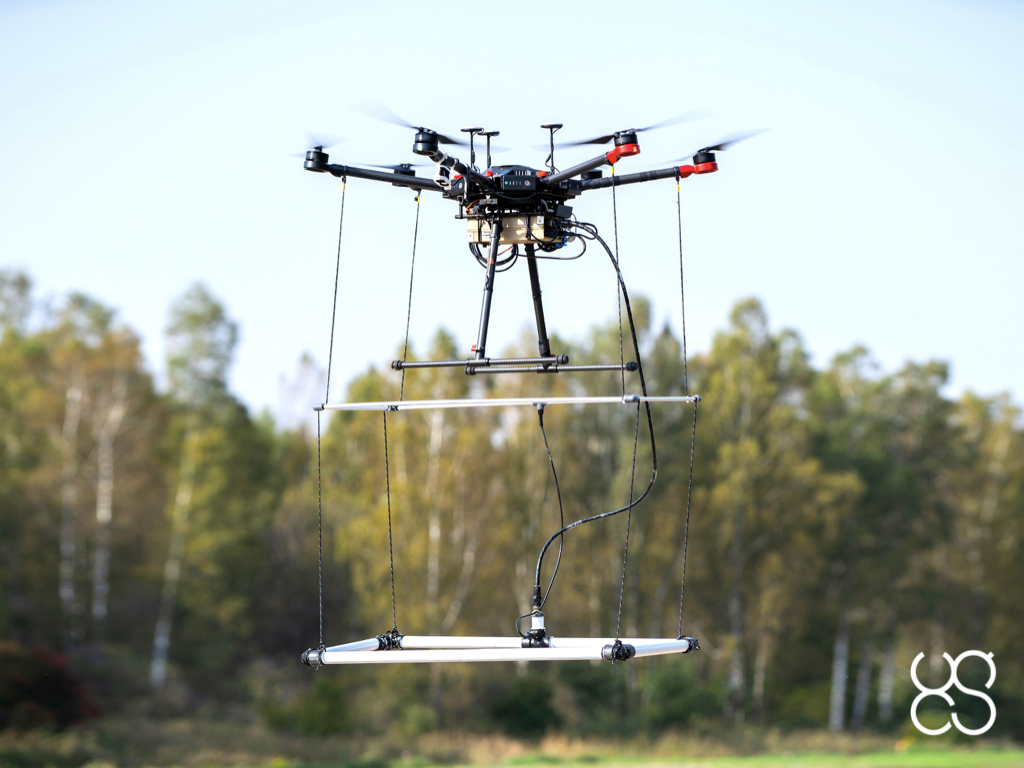
\includegraphics[width=\linewidth]{figs/Huirui/metal_detector_drone.png}
        \caption{UAV-mounted metal detector system\protect\footnotemark.}
        \label{fig:metal_detector_drone}
    \end{subfigure}
    \hfill
    \begin{subfigure}[b]{0.48\linewidth}
        \centering
        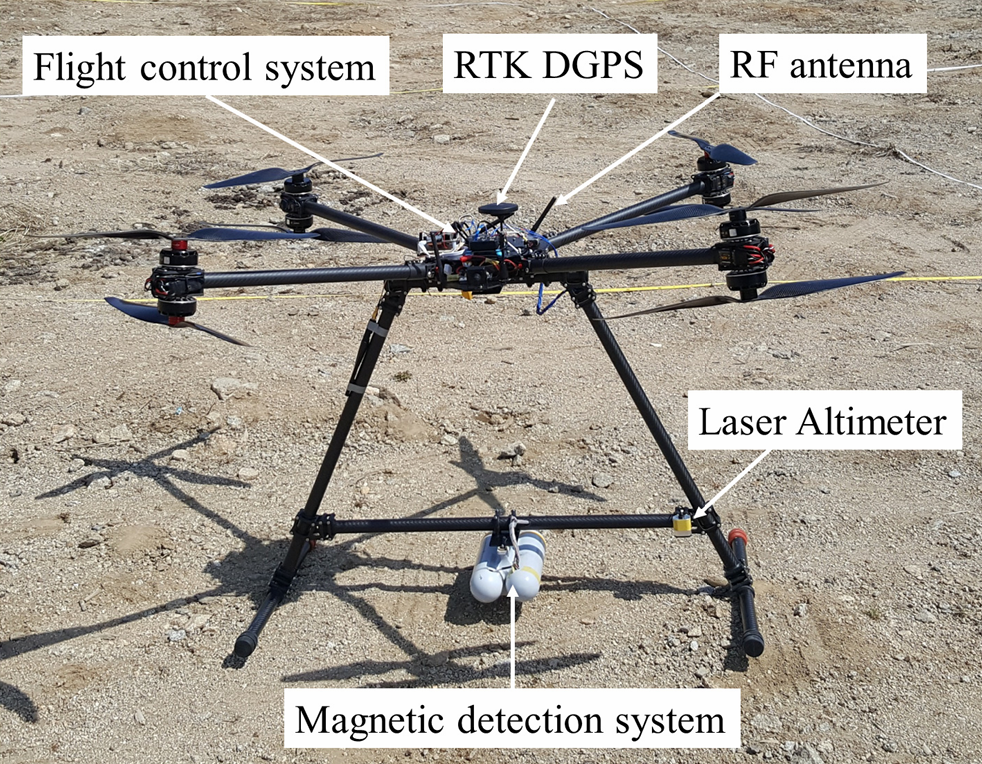
\includegraphics[width=\linewidth]{figs/Huirui/magnetometer_drone.png}
        \caption{Drone-based magnetometer platform~\cite{yoo2020drone}.}
        \label{fig:magnetometer_drone}
    \end{subfigure}
    \caption{Examples of UAV platforms integrating electromagnetic sensors for landmine detection.}
    \label{fig:emi_uav_examples}
\end{figure}

\footnotetext{\url{https://www.sphengineering.com/news/sph-engineering-introduces-the-drone-integrated-metal-detection-system}}

\paragraph{Radiowave and Microwave-Based Systems}

Ground Penetrating Radar (GPR) is a non-invasive geophysical technique that uses electromagnetic waves in the microwave frequency range (typically from several hundred MHz to a few GHz) to detect subsurface anomalies~\cite{gichd2006guidebook}. Unlike EMI-based systems, which respond to conductive or magnetic properties, GPR is sensitive to variations in the dielectric properties of materials~\cite{Gooneratne2004ARO}. It operates by transmitting short-duration radio pulses into the ground via a wideband antenna. When these pulses encounter boundaries between materials with different dielectric constants—such as between soil and a buried landmine—they are partially reflected. The reflected signals are then captured by a receiving antenna, and the time delay and intensity are analyzed to estimate the depth, shape, and dielectric contrast of subsurface targets~\cite{alqudsi2021review, paik2002image}.

As the antenna is moved across the ground, successive measurements are combined to construct two-dimensional slices (radargrams) or even three-dimensional volumetric representations of the subsurface~\cite{Bruschini1997ASO}. The effectiveness of GPR depends heavily on the contrast between the dielectric properties of the object and the surrounding soil. High-frequency systems offer better resolution and are more suited for detecting small anti-personnel mines, while lower-frequency systems provide deeper penetration but at the cost of detail~\cite{gichd2006guidebook}.

\textbf{Strengths:} One of GPR’s major strengths is its ability to detect both metallic and non-metallic mines, including those with plastic casings, by sensing changes in dielectric properties~\cite{Gooneratne2004ARO}. Unlike metal detectors, GPR systems are relatively insensitive to small surface metallic debris, which helps reduce false alarm rates~\cite{gichd2006guidebook}. They also provide useful information about object depth and shape, and can generate cross-sectional or 3D images of the subsurface~\cite{Bruschini1997ASO}. GPR is widely used in archaeological surveys, utility mapping, and geology, and is well understood in terms of commercial deployment and signal processing. Modern GPR systems are compact, lightweight, and pose no radiation hazard due to their low-power operation~\cite{gichd2006guidebook}.

\textbf{Limitations:} The main limitations of GPR lie in its sensitivity to soil conditions. High soil moisture, clay content, or rough surface topology can cause strong attenuation of the radar signal, making it difficult to detect shallow or low-contrast targets~\cite{Gooneratne2004ARO}. Performance can also degrade in dry, homogeneous soils due to insufficient dielectric contrast~\cite{robledo2009survey}. The detection of small anti-personnel mines can be particularly challenging if their signal is masked by surface reflections. Additionally, GPR systems require careful tuning of frequency to balance resolution and penetration depth, and are susceptible to signal distortion caused by subsurface clutter such as rocks, roots, or air pockets~\cite{cardonalandmine}.

\textbf{Drone-Based Applications:} GPR has been widely explored for drone integration due to its capability to detect plastic-cased mines and to provide volumetric subsurface data. UAV-mounted GPR systems typically use lightweight ultra-wideband (UWB) antennas and operate at low altitude to maintain signal fidelity. Applications include detecting anti-tank and anti-personnel mines in varied terrain types, including sand, loam, and clay\footnote{\url{https://www.sphengineering.com/integrated-systems/technologies/gpr}}~\cite{vsipovs2020lightweight,cerquera2017uav,fernandez2018synthetic,amiri2012feasibility,safarov2022detection,vsipovs2020lightweight,colorado2017integrated,schreiber2019advanced,pongrac2022advanced,garcia2020airborne,prager2019application,garcia2019autonomous,burr2018design,fernandez2021development,colorado2017low,lee2023modeling,sipos2017drone,garcia2022safedrone,almutiry2020uav,schartel2018uav,bahnemann2022under,garcia2022validation,chen2023ground}. Figure~\ref{fig:gpr_uav_examples} shows two UAV-based implementations of GPR for landmine detection.

\begin{figure}[h!]
    \centering
    \begin{subfigure}[b]{0.48\linewidth}
        \centering
        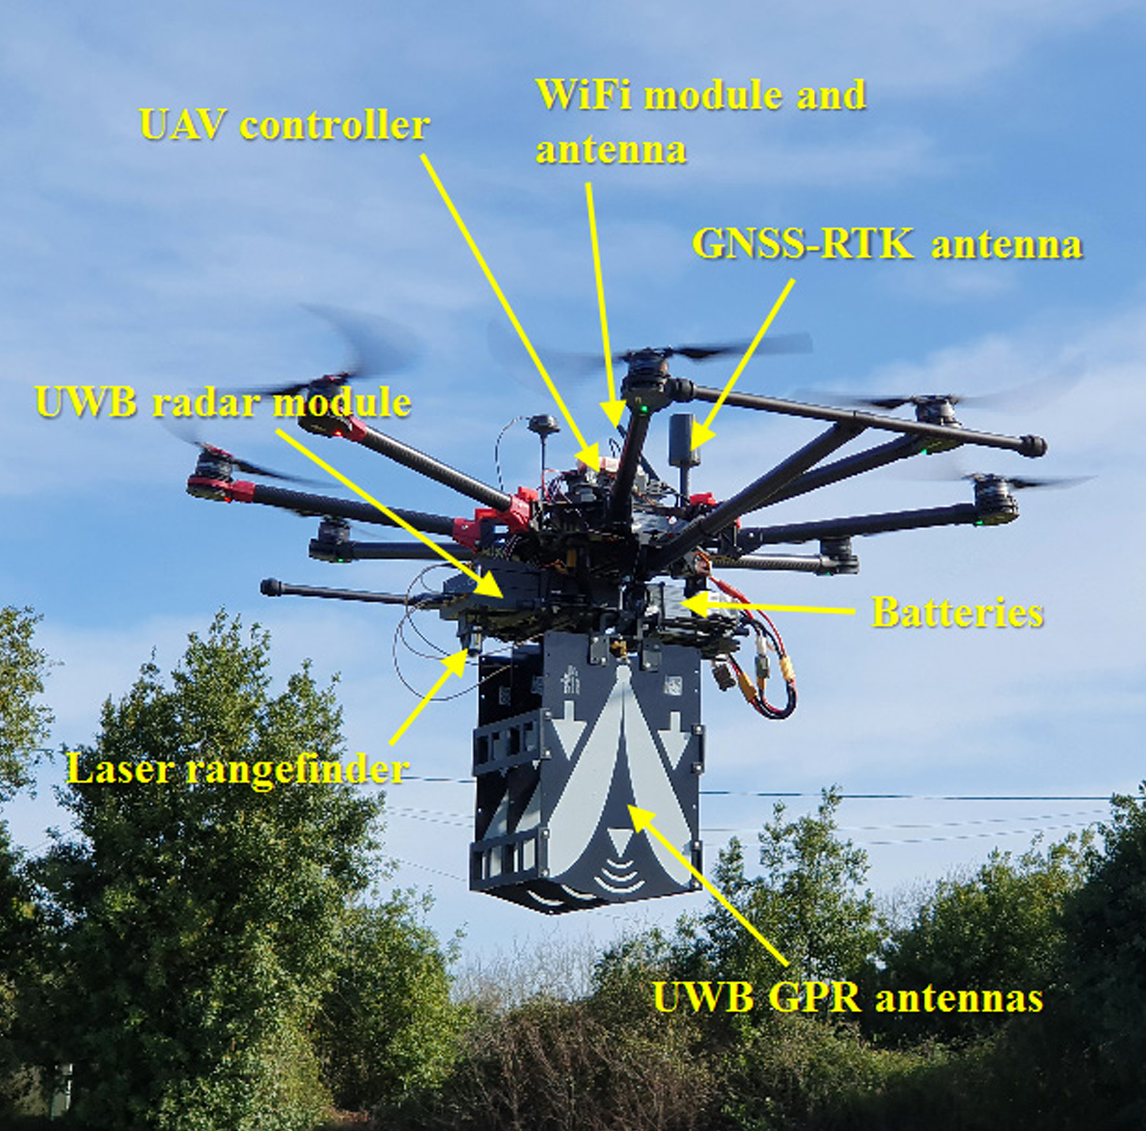
\includegraphics[width=\linewidth]{figs/Huirui/gpr_drone1.png}
        \label{fig:gpr_drone1}
    \end{subfigure}
    \hfill
    \begin{subfigure}[b]{0.48\linewidth}
        \centering
        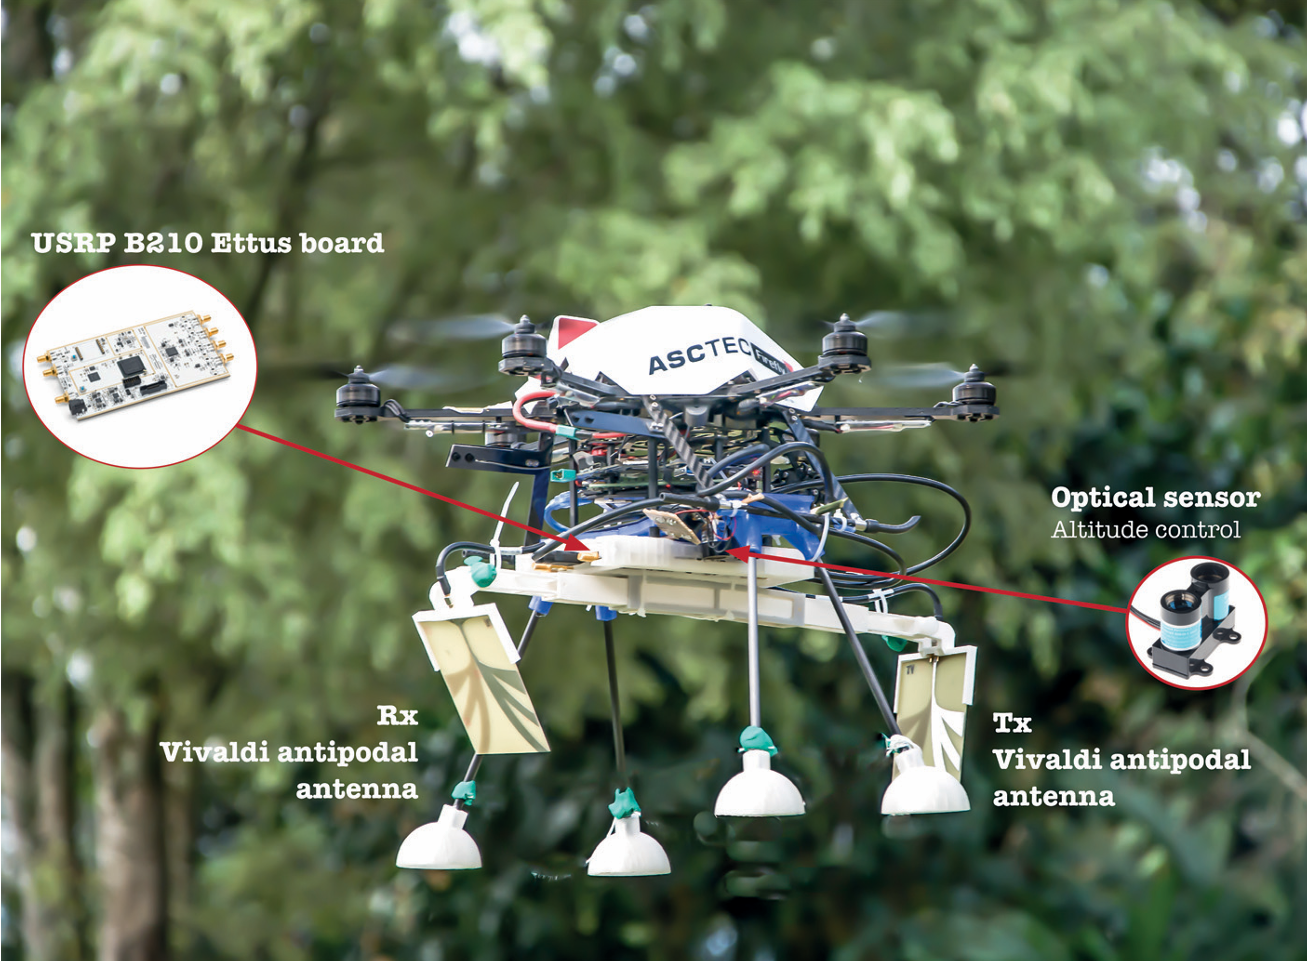
\includegraphics[width=\linewidth]{figs/Huirui/gpr_drone2.png}
        \label{fig:gpr_drone2}
    \end{subfigure}
    \caption{Examples of UAV platforms integrating GPR systems for landmine detection.~\cite{garcia2022safedrone,cerquera2017uav}}
    \label{fig:gpr_uav_examples}
\end{figure}

\subsection{Thermal Camera}

\subsubsection{Key Parameters}
- Wavelength range, frame rate, resolution, and altitude impact.

\subsubsection{Theoretical Considerations}
- Factors affecting thermal signature (e.g., burial depth, surface heating).

\subsubsection{Example Hardware and Final Selection}
- Summary of camera options and rationale for choice.

\subsubsection{Sensor Operation and Flight Parameter Configuration}
- Flying height, scanning resolution, and field of view.

- Guidelines from theory and past work to inform drone altitude and speed.
\subsection{Ground Penetrating Radar}\label{GPR_system}

\subsubsection{Fundamentals of GPR}\label{GPR_fundamental}

\gls{GPR} is a non-invasive subsurface sensing technique that detects buried objects by emitting \gls{EM} waves and analyzing their reflections. A typical \gls{GPR} system is consisted of a wideband antenna and an active sensor. The antenna emits \gls{EM} waves into the ground, and reflections are captured where there is a contrast in dielectric properties, like between soil and a buried landmine~\cite{paik2002image}.

The presence and depth of subsurface objects are inferred from discontinuities in the round-trip signal. The time delay $\Delta t$ between transmission and reception is used to estimate the distance $R$ to the reflecting object by \( R = \frac{v \cdot \Delta t}{2}\) where $v$ is the wave velocity in the medium depending on soil properties~\cite{paik2002image}.

To visualize \gls{GPR} data, three types of scans are commonly used: \textbf{A-scan}, \textbf{B-scan}, and \textbf{C-scan}. A-scans represent 1D reflections at a single point, showing signal amplitude versus time delay. B-scans combine a series of A-scans along a line to form a 2D cross-sectional view of the subsurface, while C-scans stitche together multiple adjacent B-scans to generate a volumetric 3D map of the ground. 

Figure~\ref{fig:gpr_coords} illustrates the 3D coordinate system used in \gls{GPR} scanning. A-scans are taken vertically into the ground at positions $(x’, y’)$. Moving the sensor along the $x$-axis forms a B-scan, and sweeping across $y$-axis yields a C-scan. A sample B-scan image is shown in Figure~\ref{fig:gpr_bscan}, where hyperbolic reflection patterns indicate buried objects~\cite{paik2002image}.

\begin{figure}[h!]
    \centering
    \begin{subfigure}[b]{0.48\linewidth}
        \centering
        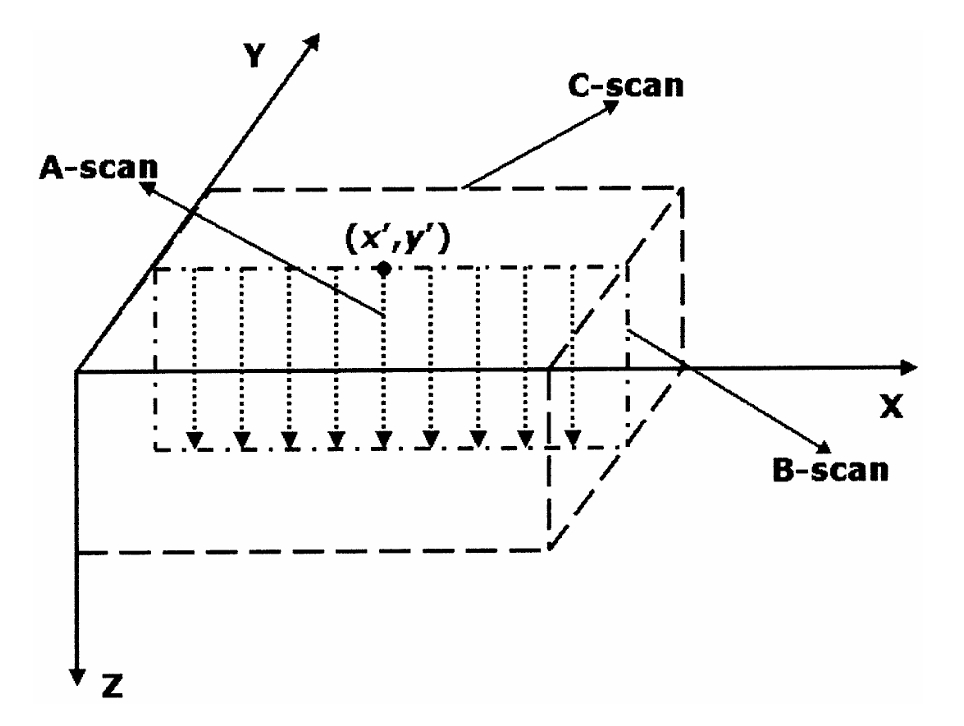
\includegraphics[height=5cm]{figs/Huirui/gpr_coords.png}
        \caption{Coordinate convention for GPR scanning.}
        \label{fig:gpr_coords}
    \end{subfigure}
    \hfill
    \begin{subfigure}[b]{0.48\linewidth}
        \centering
        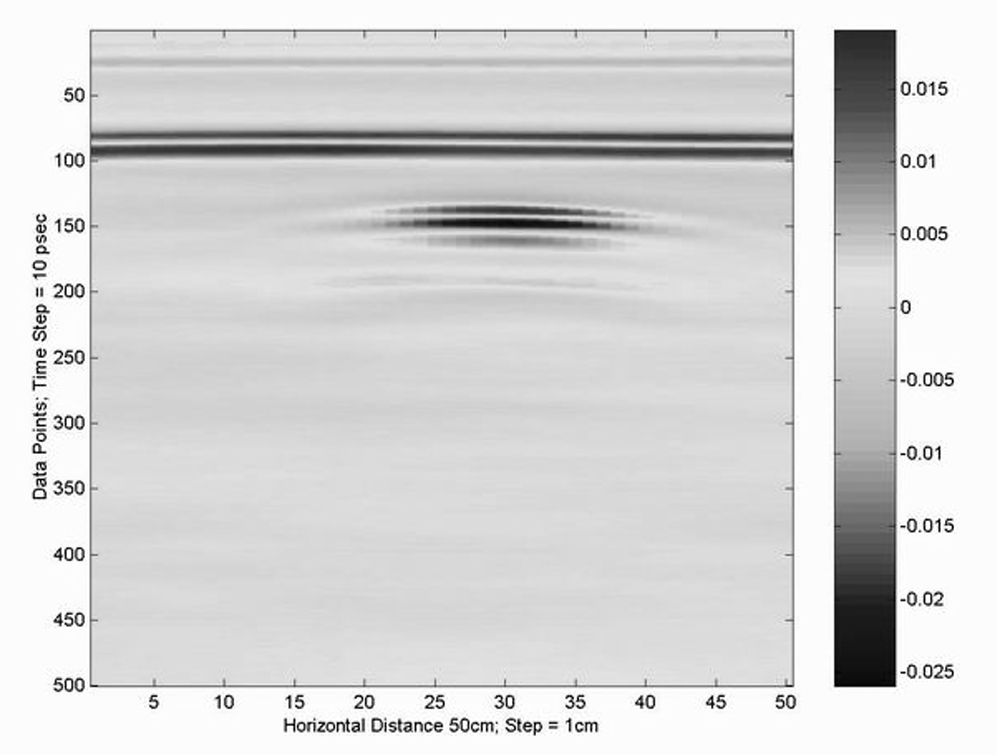
\includegraphics[height=5cm]{figs/Huirui/gpr_bscan.png}
        \caption{Example of a B-scan.}
        \label{fig:gpr_bscan}
    \end{subfigure}
    \caption[Visualization of GPR data acquisition and interpretation]{Visualization of GPR data acquisition and interpretation~\cite{paik2002image}.}
\end{figure}

Since our project focuses on localizing and estimating the depth of landmines rather than reconstructing their full 3D geometry, we collect and process only \textbf{B-scan} data from the \gls{UAV} \gls{GPR} platform.




\subsubsection{GPR Performance Factors}\label{GPR_Factors}

The performance of a \gls{GPR} system for \gls{UAV}-based landmine detection depends on a variety of factors that influence its resolution, penetration depth, and system complexity. These include waveform generation methods, operating frequency and bandwidth, spatial resolution metrics, antenna design, signal processing techniques such as \gls{SAR}, and orientation of the radar with respect to the ground surface. This section outlines the main design parameters and discusses their implications for airborne \gls{GPR} deployment.


\paragraph{Waveform Type}

The waveform type determines how \gls{GPR} transmits and receives \gls{EM} signals plays a critical role in determining resolution, hardware requirements, and system robustness. The three most common waveform types are summarized below:

\begin{itemize}
    \item \textbf{Impulse (pulsed)} \gls{GPR} transmits ultra-short pulses with broad spectral content, enabling ultra-wideband (UWB) operation and high-resolution imaging. These systems are elatively simple and cost-effective but require a \gls{ADC} or a subsampling receiver to process the wide bandwidth~\cite{chen2023ground,sipos2017drone}.

    \item \textbf{\gls{FMCW}} \gls{GPR} emits a continuous chirp signal with linearly increasing frequency over time. This approach offers better average transmitted power and improved \gls{SNR}, but requires more complex hardware and is more vulnerable to phase noise and motion errors~\cite{burr2018design}.
    
    \item \textbf{\gls{SFCW}} \gls{GPR} steps through discrete frequencies and collects reflections in the frequency domain. The data are then converted into time-domain signals via inverse Fourier transform. While achieving high \gls{SNR} and reduced \gls{ADC} requirements, \gls{SFCW} systems often perform poorly in \gls{UAV} applications due to weak ground coupling and strong surface reflections~\cite{tronca2018comparison}.
\end{itemize}


\paragraph{Centre Frequency, Bandwidth, Resolution, and Penetration Depth}

The centre frequency and bandwidth of a radar signal are key parameters about the \gls{GPR} system’s resolution and penetration depth. 

In general, lower frequencies (e.g., < 1 GHz) enhance penetration depth but limit resolution. Higher frequencies (e.g., > 2--3 GHz) improve resolution but attenuate quickly, especially in moist or conductive soils. For example, a \gls{GPR} operating at 3~GHz may penetrate up to 0.5 m in dry soil, but only a few centimeters in wet environments~\cite{9758040}. This trade-off is illustrated in Figure~\ref{fig:freq_tradeoff}, where increasing frequency improves resolution (represented as gray circles becoming smaller) at the cost of reduced sensing depth.

\begin{figure}[H]
    \centering
    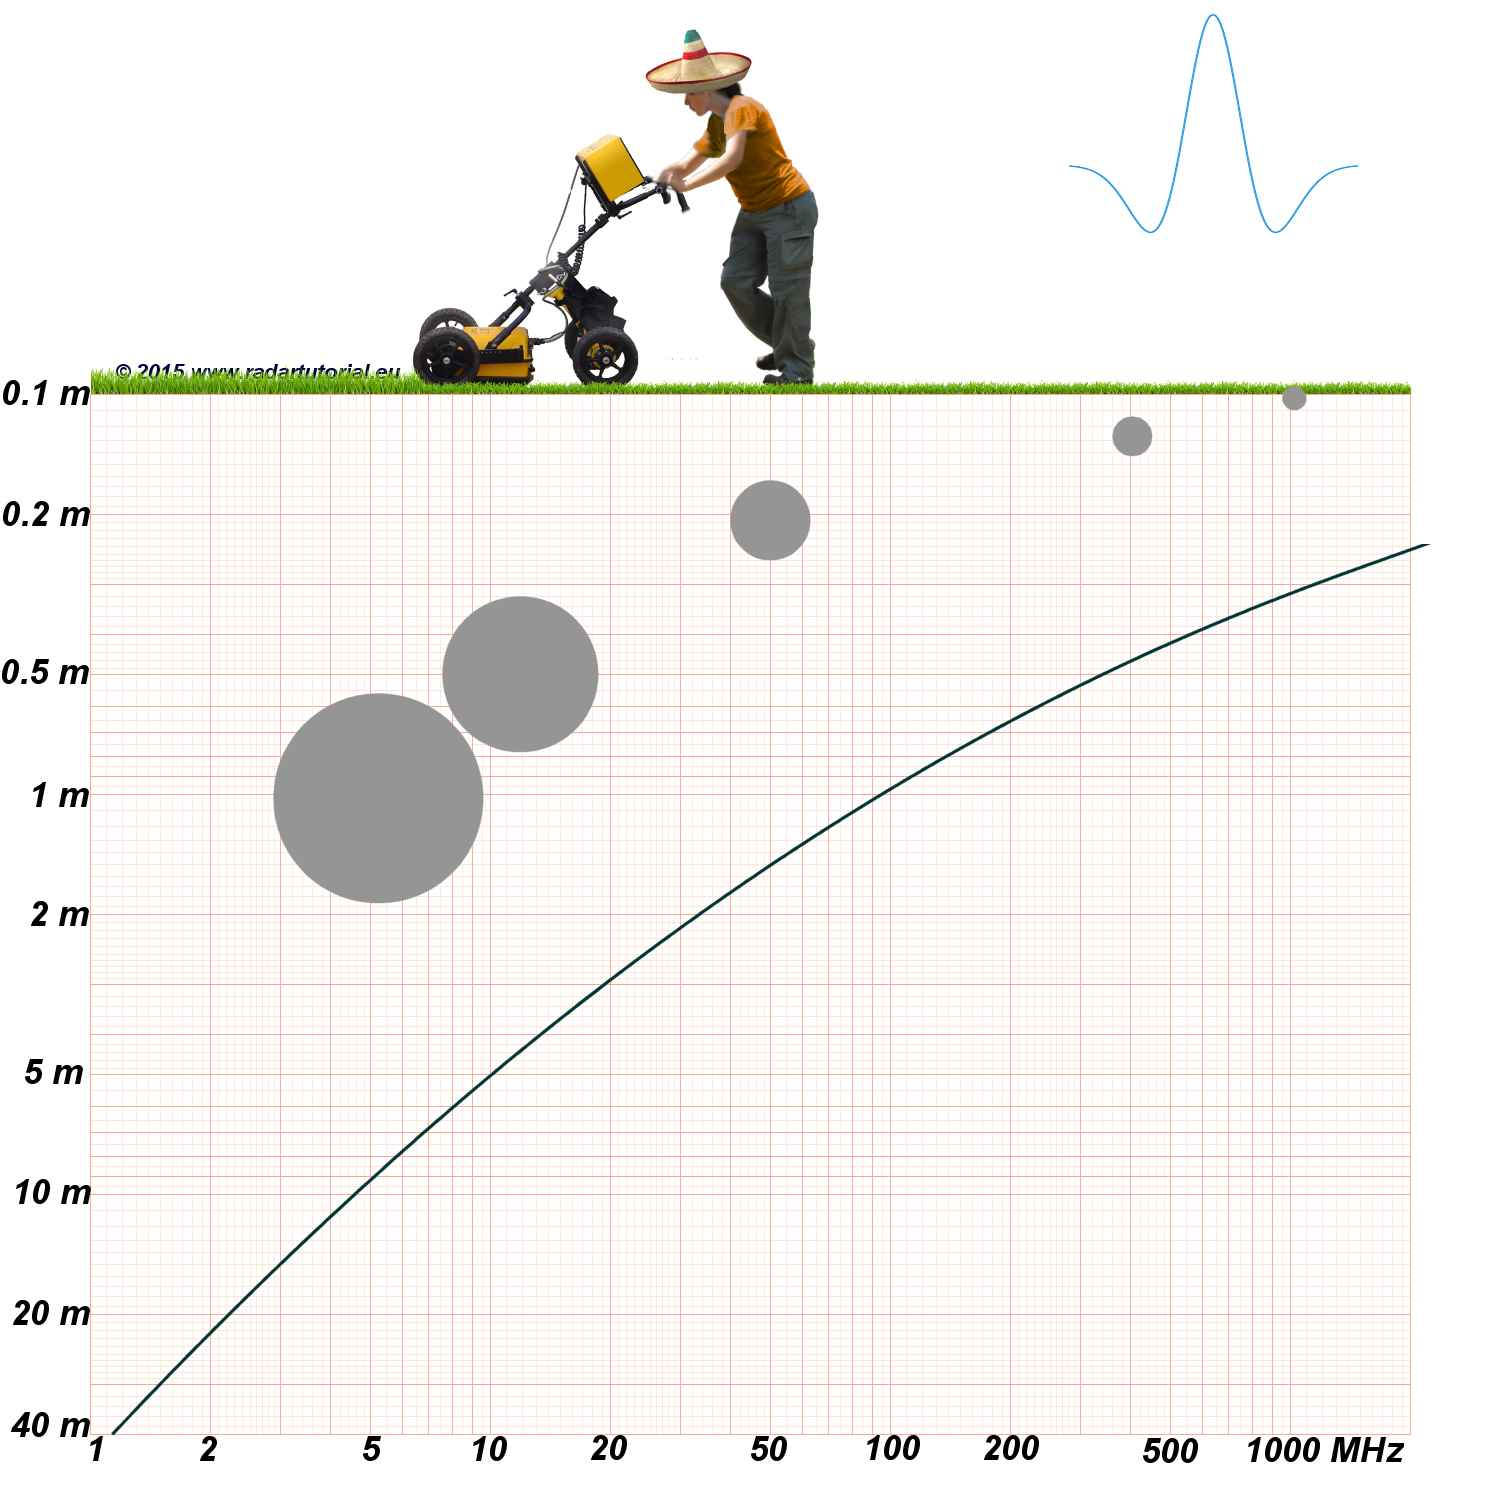
\includegraphics[width=7cm]{figs/Huirui/freq_tradeoff.png}
    \caption[Frequency, resolution, and penetration depth trade-off]{Frequency, resolution, and penetration depth trade-off\protect\footnotemark.}
    \label{fig:freq_tradeoff}
\end{figure}
\footnotetext{\url{www.radartutorial.eu}}


The radar’s bandwidth, defined as the difference between the maximum and minimum frequencies $B = f_{\text{max}} - f_{\text{min}}$, determines the system’s range (or depth) resolution $\Delta r$, which is the ability to distinguish between objects at different depths along the same vertical axis. In free-space conditions where the wave velocity $v_p = c$ (the speed of light), the range resolution $\Delta r$ is approximated by: \(\Delta r = \frac{c}{2B}~\cite{9758040}\)

Cross-range or lateral resolution $\Delta l$ defines the radar’s ability to distinguish adjacent objects at the same depth. It depends on the central wavelength $\lambda_c$, aperture size $L_{\text{ap}}$, and antenna-to-target distance $R$, and is approximated as: \(\Delta l = \frac{R \cdot \lambda_c}{L_{\text{ap}}}~\cite{9758040}\)



\paragraph{Antenna Size}

The physical size of a \gls{GPR} antenna is closely linked to the operating frequency, with lower frequencies requiring larger antennas. A rough estimate of the minimum antenna length is given by: \(L_{\text{antenna}} \approx \frac{\lambda_{\text{min}}}{2}\), where $\lambda_{\text{min}}$ is the wavelength of the minimum \gls{GPR} frequency~\cite{burr2018design}.

This relationship introduces a trade-off between penetration depth and physical size: lower frequencies penetrate deeper but require larger antennas, which may exceed the payload and form-factor limits of \gls{UAV} platforms.


\paragraph{SAR Processing}

Traditional \gls{GPR} systems have limited cross-range resolution due to the small sizes of antennas. \gls{SAR} addresses this limitation by coherently integrating radar echoes collected along the \gls{UAV}’s flight path, synthesizing a larger aperture, and significantly improving lateral resolution. This is especially beneficial for \gls{UAV}-based \gls{GPR} where antenna size and weight are constrained~\cite{9758040}.

Among \gls{SAR} algorithms, \textbf{\gls{BP}} is particularly suited for \gls{UAV} applications due to its robustness to irregular trajectories and non-uniform sampling. \gls{BP} operates by summing radar echoes along computed time-delay curves for each focal point. As shown in Figure~\ref{fig:bp_geometry}, radar signals $e_1(x_p, t)$ are collected at multiple \gls{UAV} positions $x_p$. The round-trip travel time $\tau_{m,n,p}$ from the transmitter to a target point $(x_n, z_m)$ and back is used to time-shift and coherently sum these signals by \(e_2(x_n, z_m) = \sum_{p=1}^{P} e_1(x_p, \tau_{m,n,p})\) and \(\tau_{m,n,p} = \frac{2R_a}{c} + \frac{2R_b}{v}\) where $R_a$ and $R_b$ are distances through air and soil respectively, $c$ is the speed of light, and $v$ is the wave velocity in soil. This delay-and-sum approach transforms hyperbolic reflections in conventional B-scans (like Figure~\ref{fig:gpr_bscan}) into focused point targets, improving subsurface interpretability. However, the method is computationally intensive and not ideal for real-time onboard processing~\cite{lei2014multi}.

\begin{figure}[H]
    \centering
    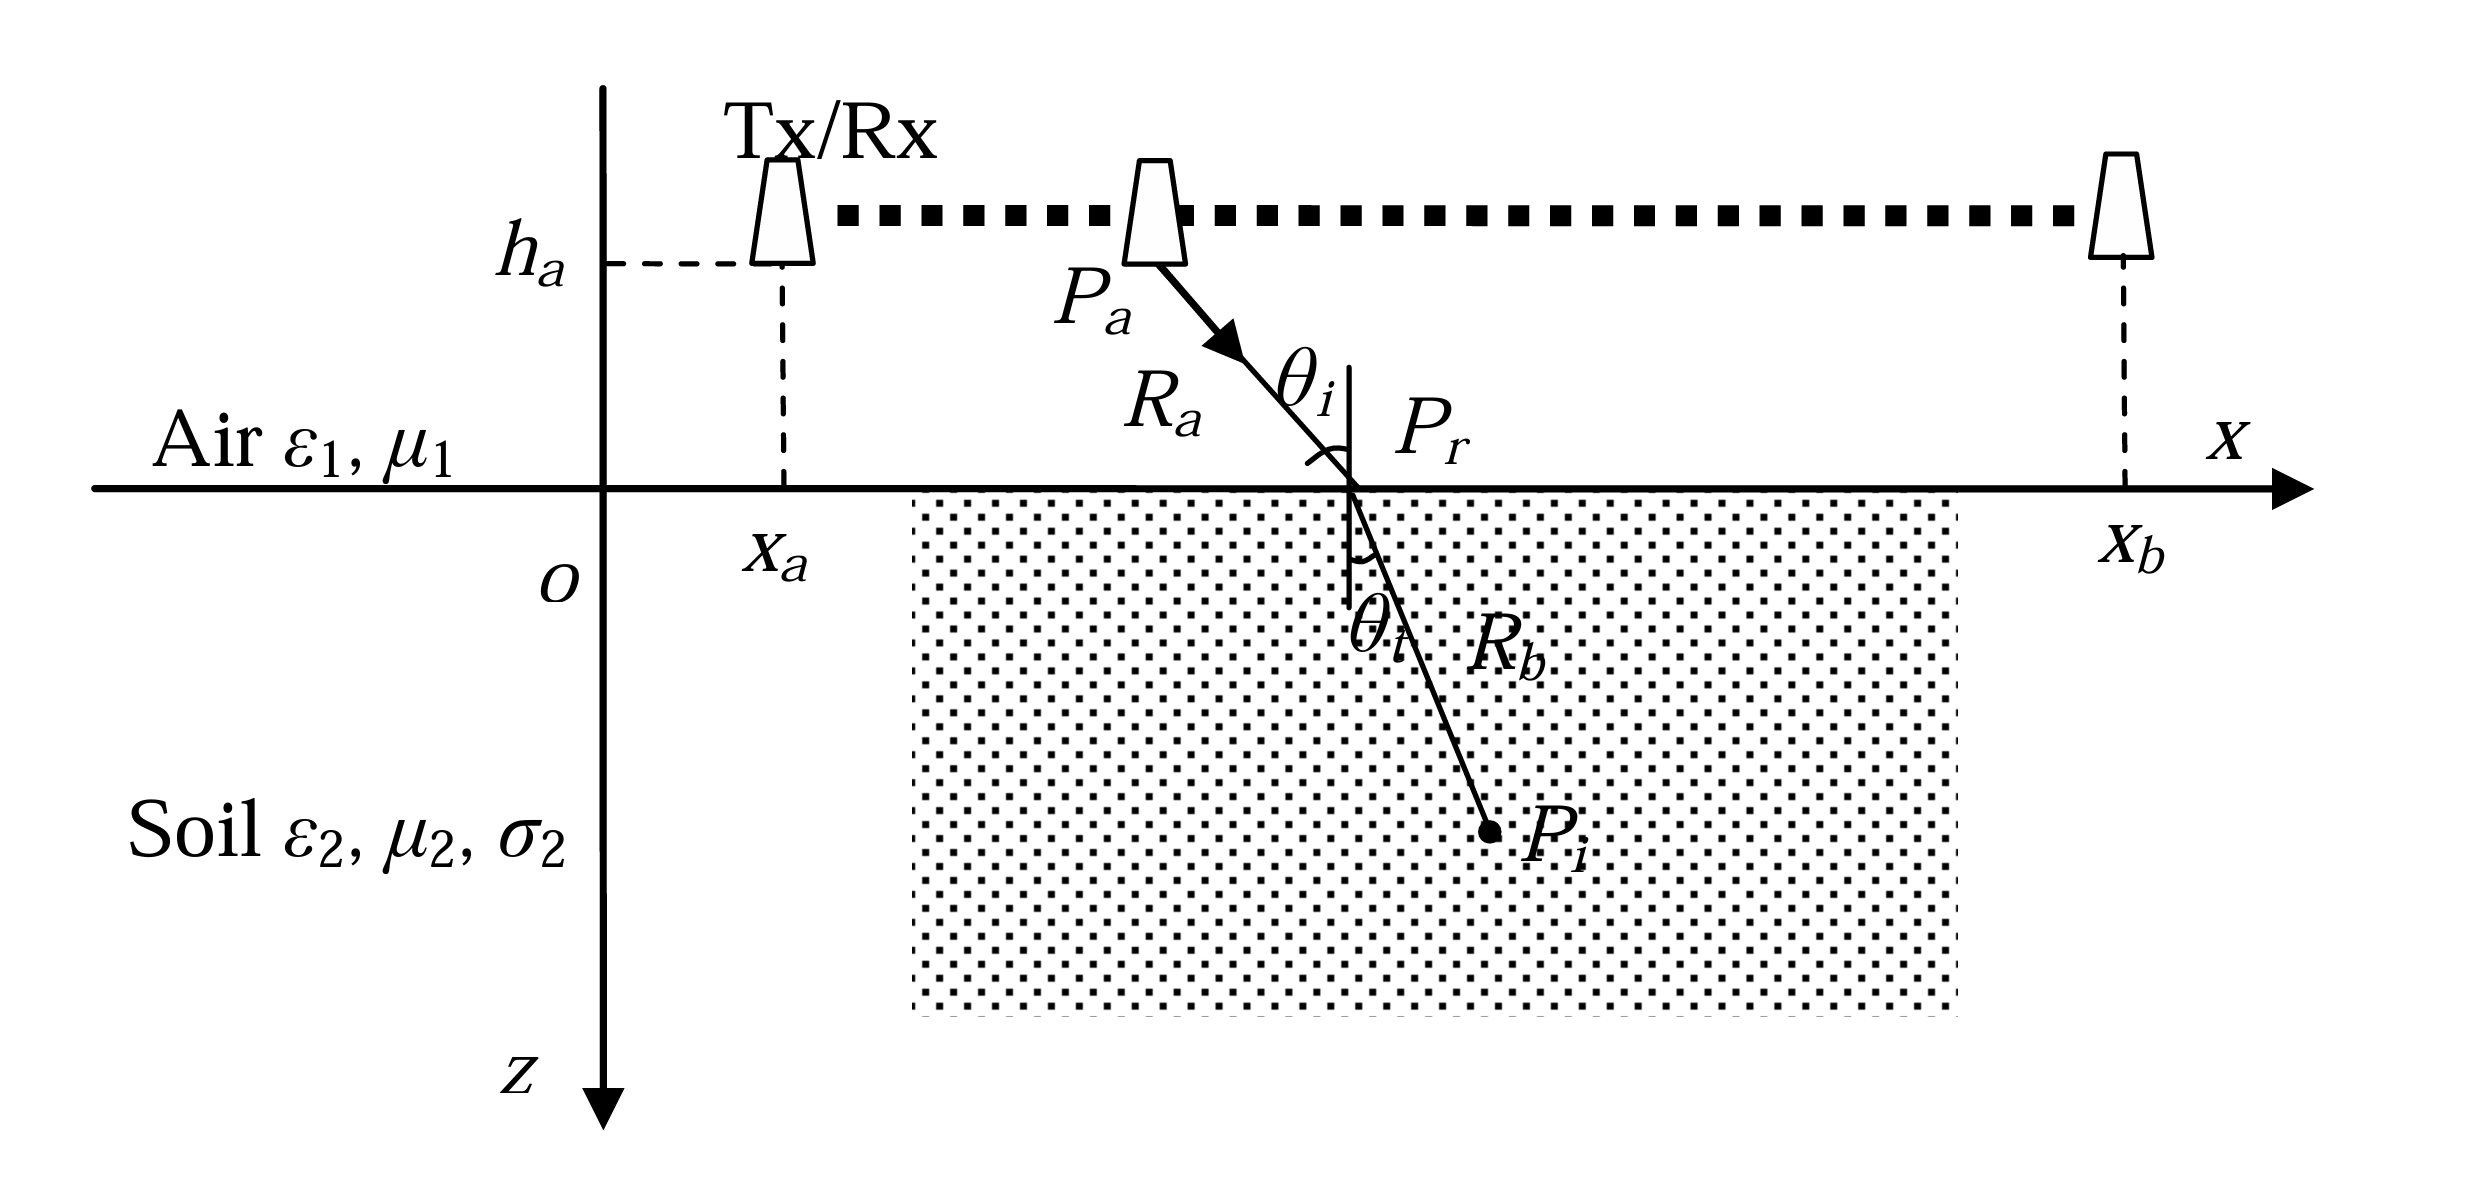
\includegraphics[height=5cm]{figs/Huirui/bp_geometry.png}
    \caption[BP SAR imaging geometry]{Illustration of BP SAR imaging geometry~\cite{lei2014multi}.}
    \label{fig:bp_geometry}
\end{figure}


\gls{SAR} can operate in different beam-steering modes depending on coverage and resolution needs (Figure~\ref{fig:sar_modes}):

\begin{itemize}
    \item \textbf{Stripmap \gls{SAR}} maintains a fixed beam relative to the \gls{UAV}, illuminating a continuous swath as the platform moves forward, which offers a balance between area coverage and resolution~\cite{moreira2013tutorial}.
    \item \textbf{Scan \gls{SAR}} periodically steers the beam to cover multiple adjacent swaths, increasing area coverage at the cost of reduced resolution~\cite{moreira2013tutorial}.
    \item \textbf{Spotlight \gls{SAR}} keeps the beam focused on a single target area, maximizing resolution but limiting area coverage~\cite{moreira2013tutorial}.
\end{itemize}

\begin{figure}[H]
    \centering
    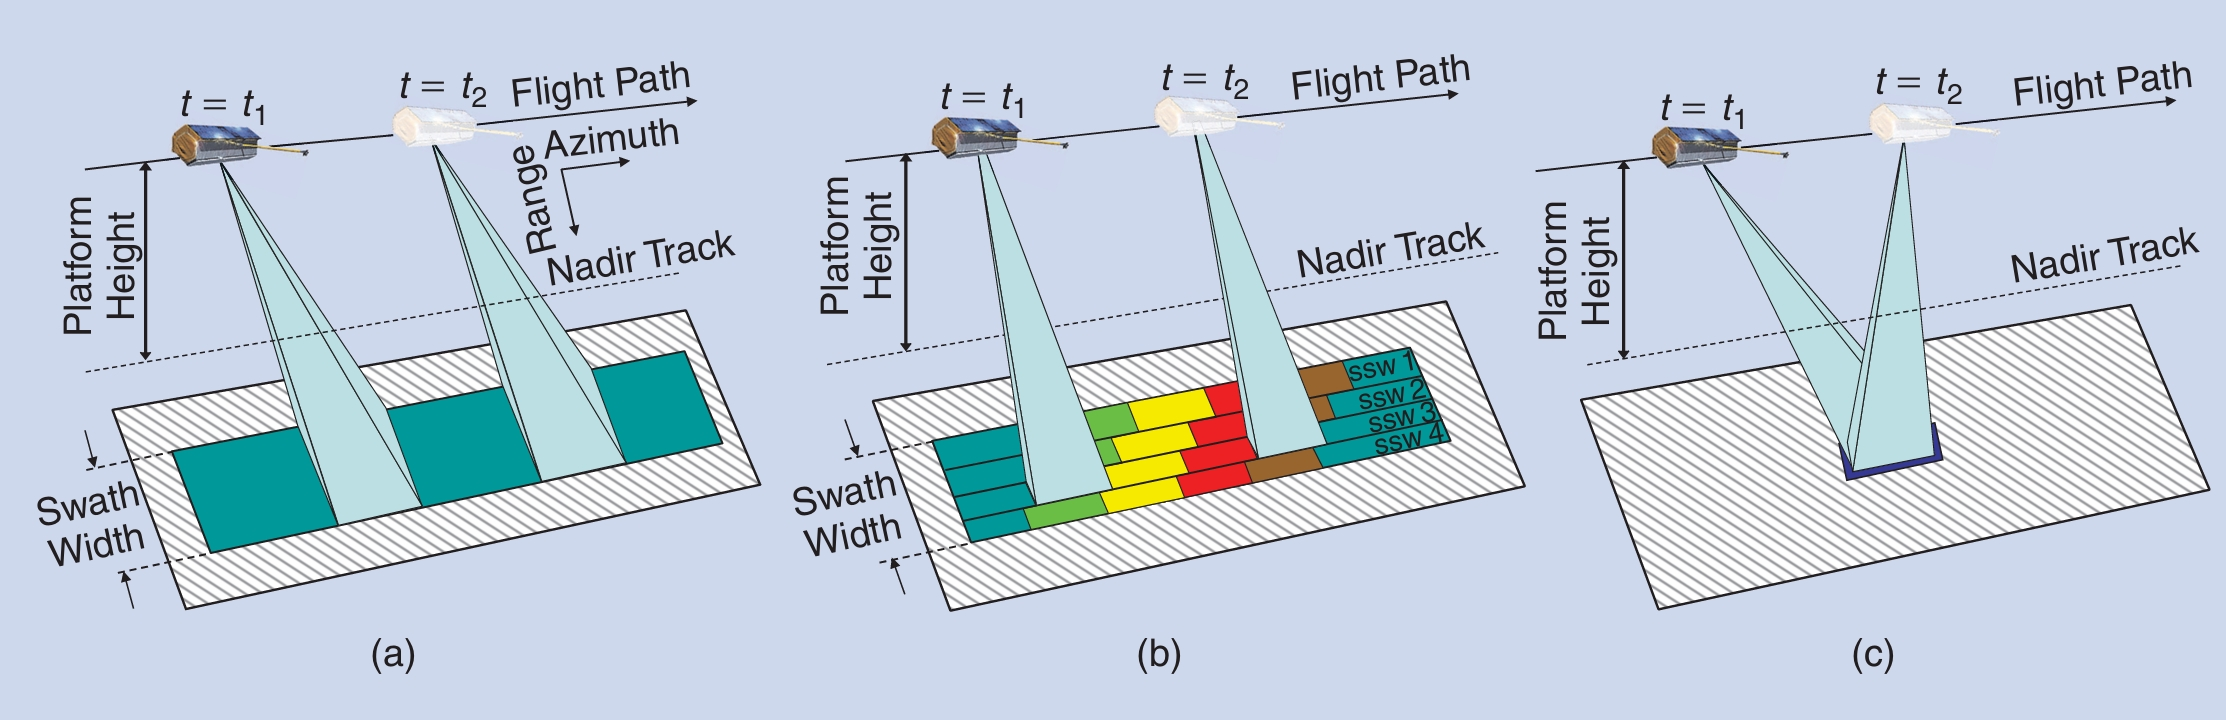
\includegraphics[height=4cm]{figs/Huirui/sar_modes.png}
    \caption[SAR operation modes]{Different SAR operation modes: (a) Stripmap SAR, (b) Scan SAR, and (c) Spotlight SAR~\cite{moreira2013tutorial}.}
    \label{fig:sar_modes}
\end{figure}


\paragraph{Radar Orientation}

The orientation of the \gls{GPR} antenna on a \gls{UAV} plays a critical role in determining both imaging performance and ease of integration. Two common configurations are illustrated in Figure~\ref{fig:GPR_Ori_modes}:

\begin{itemize}
    \item \textbf{\gls{FLGPR}} or \textbf{Side-Looking \gls{GPR}} emits waves obliquely into the ground, which reduces surface clutter. However, it receives weak backscattered signals from buried objects, requiring high dynamic range receivers and precise beam alignment~\cite{garcia2020airborne}.

    \item \textbf{\gls{DLGPR}} points antennas perpendicularly toward the ground, maximizing reflected signal strength from targets but becoming more sensitive to surface clutter~\cite{garcia2020airborne}.
\end{itemize}

\begin{figure}[H]
    \centering
    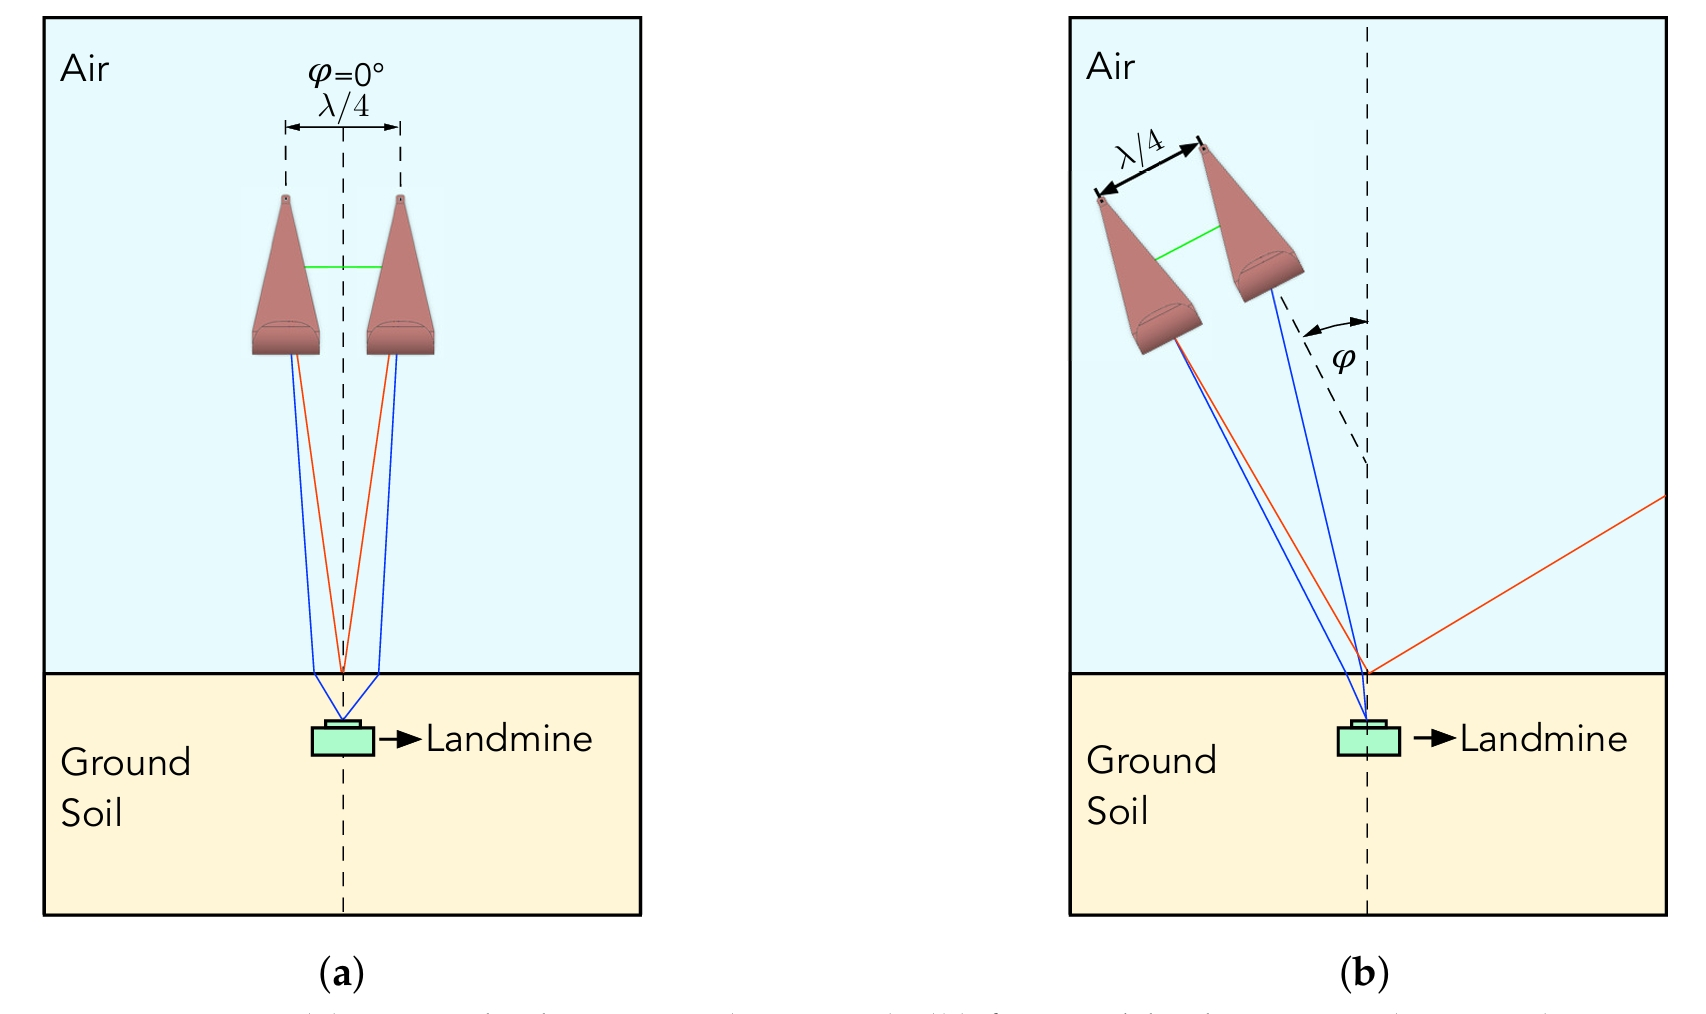
\includegraphics[height=6cm]{figs/Huirui/gpr_ori_modes.png}
    \caption[GPR orientations]{GPR orientations: (a) DLGPR, and (b) FLGPR~\cite{vsipovs2020lightweight}.}
    \label{fig:GPR_Ori_modes}
\end{figure}



\subsubsection{GPR System Design}\label{GPR_design}

While numerous \gls{GPR} architectures have been explored in previous research, most high-performance \gls{UAV}-based landmine detection systems rely on custom radar platforms. These typically incorporate \gls{SDR}, customized waveform generators, and advanced antenna arrays to maximize their environmental adaptability, resolution, and penetration~\cite{cerquera2017uav}.

In contrast, the focus of our project is to demonstrate the feasibility of integrating \gls{GPR} within a layered, multi-\gls{UAV} landmine detection framework. Given the constraints of time, budget, and hardware development, we propose the use of a \gls{COTS} impulse \gls{GPR} system for our initial implementation.

We select the \textbf{SPH Engineering Zond Aero 1000 MHz \gls{GPR}} (~1.8~kg\footnote{\label{Zond}\url{https://cdn.shopify.com/s/files/1/0596/9451/4353/files/RadSys_Zond_Aero_1000_NG_datasheet.pdf?v=1732295405}}). It operates in the 600–1300~MHz band with a center frequency of 1~GHz\textsuperscript{\ref{Zond}}, offering reasonable balance between resolution and penetration. Unlike high-frequency systems that offer fine detail at shallow depths, this system prioritizes deeper penetration—essential for detecting mines in compact or moist soils. Although its vertical resolution (around 10--15~cm) may not allow precise depth estimation, this is acceptable for our use case, where the primary goal is to confirm the existence rather than reconstruct detailed object geometry of the buried landmines.

The system uses a \textbf{\gls{DLGPR}} configuration, maximizing reflected signal power from targets and simplifying hardware integration. While \gls{DLGPR} does introduce surface clutter due to strong air–ground reflections, it can be mitigated through signal processing techniques such as Singular Value Decomposition (SVD) and migration algorithms ~\cite{garcia2024comparison}. Furthermore, \gls{DLGPR} is the most widely adopted orientation in past \gls{UAV}-\gls{GPR} applications, supporting its practical reliability ~\cite{9758040}.

To improve lateral resolution and compensate for the limited range resolution of our low-frequency radar, we apply \gls{SAR} processing in \textbf{Stripmap} mode using a \textbf{\gls{BP}} algorithm. This enables continuous scanning without beam steering, reducing \gls{UAV} control complexity. Since coherent SAR imaging requires centimeter-level positioning accuracy to align radar returns across the UAV trajectory~\cite{fernandez2018synthetic}, we ensure this through the integration of a high-precision GNSS and IMU system, as described in section~\ref{sub_sub_section:tgt_component_selection}. Real-time processing is avoided due to the computational cost of \gls{BP}; instead, raw B-scans are geo-referenced and processed offline after each flight.

This system architecture based on a down-looking \gls{COTS} impulse radar at low-frequency operation with offline \gls{SAR} processing provides a realistic and effective foundation for our system’s initial deployment. It balances feasibility with performance, while leaving room for future upgrades such as real-time \gls{SDR} control or custom radar development in subsequent project phases.



\subsubsection{GPR System Flight Configuration}\label{GPR_flight}

In our system, the \gls{GPR} drone is designed to fly at an altitude around \textbf{2~m}. This low flight height ensures a balance between maximizing power coupling into the ground and maintaining safe clearance for autonomous operations, consistent with previous \gls{DLGPR} studies on \gls{UAV} landmine detection ~\cite{schartel2018uav,9758040}.

As illustrated in Figure~\ref{fig:swath_geometry}, for our \gls{DLGPR} system ($\alpha = 90^\circ$), assuming a beamwidth (the angle between near range and far range) of $\theta = 45^\circ$, the effective swath width $W$ can be derived geometrically as \(W = 2H \cdot \tan\left(\frac{\theta}{2}\right)\). For $H = 2$~m,  $W = 1.65$~m. This value defines the effective width of ground coverage per flight strip.

\begin{figure}[H]
    \centering
    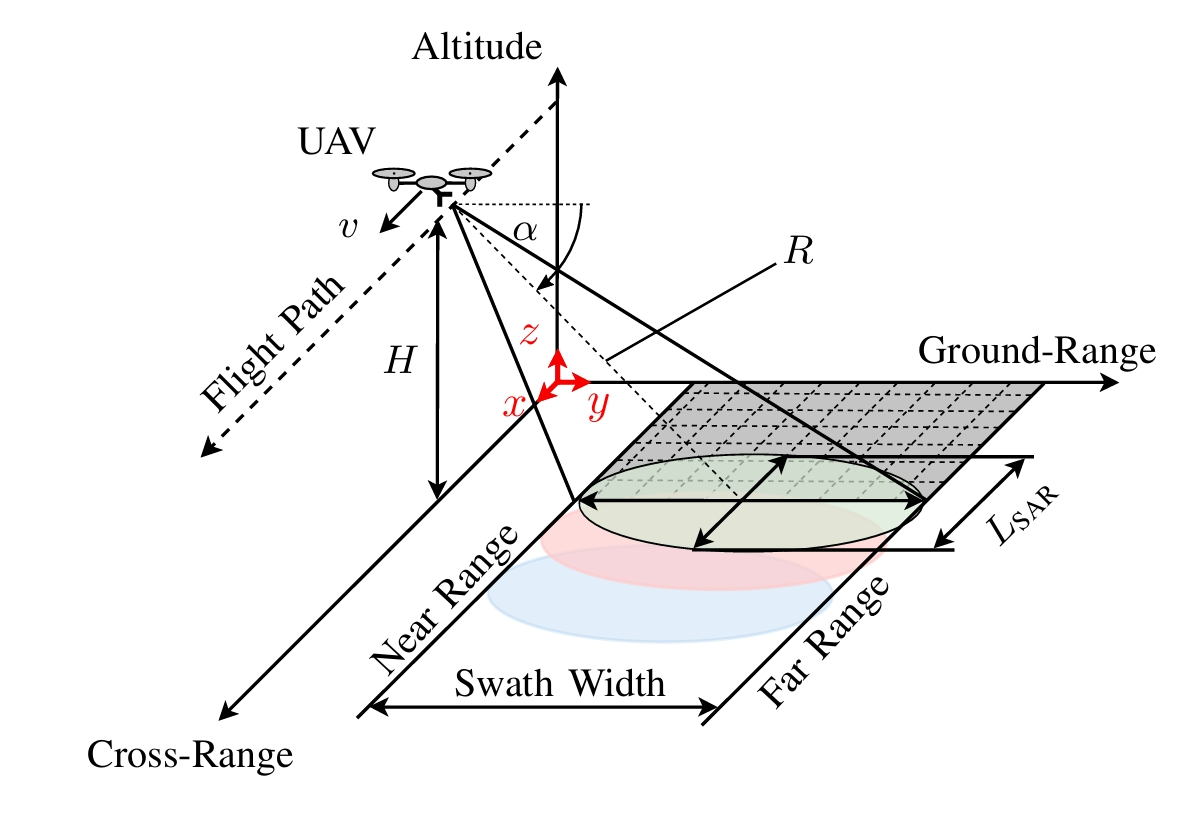
\includegraphics[height=6cm]{figs/Huirui/gpr_swath}
    \caption[Stripmap SAR geometry]{Illustration of the stripmap SAR geometry.~\cite{schartel2018uav}.}
    \label{fig:swath_geometry}
\end{figure}

To enable effective \gls{SAR} reconstruction using the \gls{BP} algorithm, radar acquisition points must satisfy the Nyquist sampling rate, which requires that the maximum spacing $\Delta x$ between successive measurements does not exceed half the wavelength corresponding to the system's maximum radar frequency: \(\Delta x \leq \frac{\lambda_{\text{min}}}{2}\)~\cite{9758040}.

For our system with a maximum operating frequency of 1.3~GHz, the minimum wavelength is approximately 23~cm, resulting in a maximum sampling interval of \textbf{11.5~cm}. Given the estimated thermal camera coverage of 9 m × 7 m mentioned in section before, assuming a zig-zag path with overlapping swath like Figure~\ref{fig:swath_geometry}, a total of \textbf{332 points} are required to fully sample one thermally flagged region. 
\subsection{Sensor Integration}

\subsubsection{Sensor Integration and Data Handling}
- Data interfaces and storage solutions (e.g., onboard SD logging).

- Software hooks for starting/stopping recording and syncing data with GPS.

\subsubsection{Preprocessing and Onboard Processing}
- Initial data cleaning or transformation (e.g., filtering GPR signals).

- Localization tagging for thermal and radar data.

- Mention potential for real-time or offline processing.

\newpage
\pagenumbering{arabic}
\fancyhead[C]{Rory Millard}
\section{Computer Vision} \label{computervision}

\subsection{Thermal Computer Vision}

This is the thermal computer vision subsection
\subsection{Thermal Simulations}

This is the thermal simulations subsection

\subsubsection{Governing Equations}
Unsteady Heat Equation

The general form of the 3D unsteady heat equation in Cartesian coordinates is:

\begin{equation}
    c_p \rho \frac{\partial T}{\partial t} = 
    \frac{\partial}{\partial x} \left( k \frac{\partial T}{\partial x} \right) + 
    \frac{\partial}{\partial y} \left( k \frac{\partial T}{\partial y} \right) + 
    \frac{\partial}{\partial z} \left( k \frac{\partial T}{\partial z} \right)
\end{equation}


where:
\begin{itemize}
    \item \( T(x,y,z,t) \) is the temperature field,
    \item \( k(x,y,z,t) \) is the thermal conductivity,
    \item \( \rho(x,y,z,t) \) is the mass density,
    \item \( c_p (x,y,z,t) \) is the specific heat capacity.
    
\end{itemize}

For piecewise constant properties $\rho, k, c_p$ this can be written as

\begin{equation}
    \frac{\partial T}{\partial t} = \alpha \left( \frac{\partial^2 T}{\partial x^2} + \frac{\partial^2 T}{\partial y^2} + \frac{\partial^2 T}{\partial z^2} \right)
\end{equation}

which can be compactly written as

\begin{equation}
    \frac{\partial T}{\partial t} = \alpha \nabla^2 T
\end{equation}



Where \( \alpha(x,y,z,t) := \frac{k}{\rho c_p}\) is the thermal diffusivity.


\subsection{Radar Computer Vision}

This is the radar computer vision subsection
\subsection{Radar Simulations}

This is the radar simulations subsection

\subsection{Data Fusion}

This is the data fusion subsection
\newpage
\fancyhead[C]{Rory Millard}
\section{Sensor Fusion} \label{fusion}



\subsection{Overview of Fusion} \label{fusion_overview}

    \noindent The late stage fusion approach was introduced in Section \ref{compvis_intro}. It is justified on the grounds of simplicity; by processing each sensor's data through individual YOLO models before merging, the network architectures are simpler. The networks can be retrained in parallel, and single points of failure are removed. 
    


    \noindent In this section, the outputs from the individual YOLO models are interpreted as probability maps, where the confidence value assigned by the YOLO model is equal to the probability of finding a landmine at that location, according to each sensor. The fusion algorithm combines the two probability maps, defined over the same geographical space, into a third map. This is done using the sensor data and environmental contextual data.

    Fusing the sensor outputs before the CNN is problematic due to irregular input sizes and the need for computationally intensive mosaicking algorithms that may introduce errors. Instead, the accurate position, pose and field of view metadata  is leveraged to project each YOLO output onto a common geographical grid. Given that these probability maps are inherently sparse (most of the probability map is zero, with occasional spikes over landmines), the projections are computationally efficient. Because the metadata is accurate, the overlapping regions of the projections will be small, and when they occur, a simple strategy—such as weighted averaging—suffices to resolve them.

    \subsubsection{The Precision-Recall Trade-off } \label{lossmatrix}

        Recall should be prioritized over precision, as a false negative in landmine detection is more dangerous than a false positive. However, no system can ensure 100\% recall, and so a mined region can never be 100\% safe. Therefore, reducing recall slightly in exchange  for a significant gain in precision can be advantageous, because the reduced recall has negligible operational impact, whilst the increased precision is associated with significant cost reduction.
\subsection{Fusion System Performance Bounds}\label{fusion_bounds}

    Independent of the specific fusion algorithm employed, the overall system performance is ultimately constrained by the intrinsic capabilities of the individual sensors. A Naive Bayes framework is adopted to establish performance estimates. The Naive Bayes approach assumes conditional independence between sensors, allowing for straightforward analytical expressions of posterior probabilities. While this simplification may not perfectly capture all sensor interactions, it provides tractable mathematics that yield conservative performance estimates; algorithms that are not limited by conditional independence, and have access to domain knowledge, will perform better than Naive Bayes for fusion.

    \subsubsection{Theoretical Framework}
        
        The following key parameters and their probabilistic interpretation, are defined: the prior mine density $\rho_0 = P(\text{Mine})$, the set of locations that have been flagged by the thermal sensor \(\mathcal{T}^+\), the thermal sensor's recall $R_T = P(\mathcal{T}^+\mid\text{Mine})$ , and its false positive rate $F_T = P(\mathcal{T}^+ \mid \overline{\text{Mine}})$. Similarly, the radar sensor is characterized by its recall $R_R$ and false positive rate $F_R$ with analagous interpretations. Following thermal scanning, the mine density in the flagged region ($\rho_1$), can be found with Bayes rule:
        \begin{equation}
        \rho_1 = P(\text{Mine} \mid \mathcal{T}^+) =\frac{P(\mathcal{T}^+\mid\text{Mine})P(\text{Mine})}{P(\mathcal{T}^+\mid\text{Mine})P(\text{Mine})+ P(\mathcal{T}^+\mid \overline{\text{Mine}})P(\overline{\text{Mine}})} =\frac{R_T \rho_0}{R_T \rho_0 + F_T (1 - \rho_0)}
        \end{equation}
        
        \paragraph{Mine Densities} 
        

            Note the use of mine densities (\(\rho\)) rather than the nominal precision values reported in Section \ref{compvis_implementation}. This is because of the class imbalance discussed in Section \ref{class_imbalance}. The nominal precision derived from an imbalanced dataset is misleading when applied to real-world conditions. Instead, a full Bayesian treatment that incorporates the prior distribution over mine density is used. This enables the accurate updating of mine density after thermal screening, giving \(\rho_1\), and then after radar verification, giving \(\rho_2\), thereby mitigating the effects of class imbalance.

    \subsubsection{Bounds on Precision and Recall}
    
        \paragraph{Precision} Under the Naive Bayes framework, the expected system precision after fusion equals the posterior mine density after both sensors have flagged an area. The radar sensor refines the density from $\rho_1$ to $\rho_2$, and the expected precision after fusion is:
        \begin{equation}
        \label{eq:rho_2}
        P_\text{F} = \rho_\text{2} = \frac{R_\text{R} \rho_\text{1}}{R_\text{R} \rho_\text{1} + F_\text{R} (1-\rho_\text{1})} \text{, where }         \rho_\text{1} = \frac{R_\text{T} \rho_\text{0}}{R_\text{T} \rho_\text{0} + F_\text{T} (1-\rho_\text{0})}.
        \end{equation}
        
         The upper bound is the radar's intrinsic precision $P_\text{R}$, giving \textbf{precision bounds of } $\rho_\text{2} \leq P_\text{sys} < P_\text{R}$
         
        \paragraph{Recall} The Naive Bayes system recall can similarly be found by considering the intrinsic recalls of each sensor, and is a lower bound on the true system recall. Because the radar sensor only scans regions flagged by the thermal sensor, the NB system recall is the product of the individual recalls \(R_\text{sys} = R_\text{T} R_\text{R}\), 
        which  cannot exceed $R_\text{T}$. This gives the \textbf{bounds on the fused system's recall as} $R_\text{T}R_\text{R}\leq R_\text{sys}< R_\text{T}$.
    
    \subsubsection{Naive Bayes Fusion: Quantifying Bounds} \label{Rory_quantifying_bounds}
    
        Using the YOLO model performance metrics in Table \ref{tab:sensor_comparison}, and a prior landmine density of 2\% ($\rho_0 = 0.02$), the following values are obtained: $R_T = 0.919,~ F_T = 0.15,~ R_R = 0.833,~ F_R = 0.085.$ These values are used to calculate the posterior density after thermal screening and subsequent radar scanning, using Equation \ref{eq:rho_2}:
        \[
        P_{sys} \geq \rho_2 = \frac{R_R \rho_1}{R_R \rho_1 + F_R (1-\rho_1)} = \frac{0.833 \times 0.112}{0.833 \times 0.112 + 0.085 \times 0.888} \approx 0.553.
        \]
        
        Therefore, this fusion process concentrates the mine likelihood from an initial 2\% to \textit{at least} 55.3\% in the regions flagged by the radar sensor—\textbf{a  27.7× improvement over indiscriminate "blind" demining}. The expected system recall is $R_{sys} \geq R_T \times R_R \approx 0.919 \times 0.833 \approx 0.765$, indicating a maximum recall drop of about $0.919 - 0.765 \approx 15.3\%$ compared to using just the thermal sensor alone.


    \subsubsection{Implications for System Design}

        \paragraph{Benefit of the GPR Sensor}
        
            
            When the radar sensor is included as part of the layered architecture, the system precision is increased approximately 5 times, with only a marginal 15.3\% drop in recall. This trade-off is justified, as a modest reduction in recall has negligible operational impact (discussed in Section \ref{fusion_overview}), whilst the boost in precision dramatically reduces operational costs, which is mentioned in Section \ref{financing}. Therefore it is crucial to have the radar sensor.
                
        \paragraph{Benefit of the Layered Approach} \label{Benefit of the Layered Approach}
        
            The layered approach, where the radar sensor only probes the points flagged by the thermal sensor, enables the radar sensor to operate over a much smaller region, covering only $\rho_1 \approx 11.2\%$ of the total land area. In contrast, if both sensors were applied in parallel, with the radar sensor scanning the entire area, the detection time and hence cost would increase much (the radar sensor is significantly slower - Section \ref{sec:msp_comparison_manual_demining}), for only a slight improvement in recall and a negligible gain in precision. Therefore, the layered approach is a very efficient way of incorporating the radar sensor. 

            

        
\subsection{Explicit Fusion Algorithm Selection}

        An explicit fusion algorithm is required to intelligently combine the thermal and radar probability maps, \(\mathcal{P}_\text{thermal}(x, y)\) and \(\mathcal{P}_\text{radar}(x, y)\), respectively, into a final probability map, \(\mathcal{P}_\text{fused}(x, y)\), over the geographical area of interest. The selection of the fusion algorithm determines where the performance of the overall system lies within the bounds from Section \ref{fusion_bounds}, and requires careful consideration of the underlying assumptions and limitations of each method.
    
    \paragraph{Naive Bayes}
    
        An initial approach might be to use a Naive Bayes fusion algorithm. This approach was used as a conservative estimate on performance in Section \ref{fusion_bounds}, and assumes conditional independence between the sensor probability maps given the presence or absence of a landmine. 
        
        However, this assumption is fundamentally flawed in this context. The thermal and radar sensor readings are not independent; they are intrinsically linked by underlying causal physics. Factors such as soil moisture, ambient temperature, and vegetation cover influence both thermal signatures and radar reflections in complex, deterministic ways. A Naive Bayes model is incapable of capturing these dependencies, leading to inaccurate fusion results. This is validated in Section \ref{compvis_anfisvalid}.
    
    \paragraph{Kalman Filter}
    
        Similarly, the Kalman Filter, while offering a mathematically elegant framework for optimal linear estimation with Gaussian noise \footnote{\url{https://en.wikipedia.org/wiki/Kalman_filter}}, is ultimately unsuitable for this application. The Kalman Filter can model the sensor covariance \textit{statistically} but cannot encode causal, physical rules like \textbf{"low soil moisture fraction amplifies the thermal detectability"} (Section \ref{thermal_sensitivity}). This limits robustness in novel environments. More fundamentally though, the Kalman Filter's assumption of \textit{unbounded} Gaussian noise is violated in this case, where the variables are \textit{bounded} sensor confidence values, \(\mathcal{P}_{\text{thermal}}, \mathcal{P}_{\text{radar}} \in [0,1]\). Truncation of the output would introduce bias.
    
    \paragraph{Neural Network}

        A Neural Network (NN), as a universal function approximator, can learn arbitrarily complex mappings between sensor inputs and fused outputs. However, a standard NN cannot include domain knowledge without extensive training data. Even with ample data, a standard NN models the statistical behaviour of the physics, rather than the underlying causal mechanisms. This lack of domain understanding would cause poor performance in novel environments, for example: when the soil is frozen, there is no thermal contrast, so the thermal sensor data provides no useful information for buried landmine detection (this is used as a fuzzy rule in Section \ref{fuzzy_rules}).


    \paragraph{ANFIS}

        The Adaptive Neuro-Fuzzy Inference System (ANFIS) \cite{jang1993anfis} addresses the limitations of prior methods by hybridizing neural networks and physics-grounded fuzzy logic. Unlike Naive Bayes, ANFIS explicitly models dependencies between sensors through rules representative of causal physical relationships. By constraining solutions to physically plausible outcomes—such as suppressing thermal confidence in frozen soils—ANFIS can achieve robust fusion even in novel environments. The network effectively \textbf{learns the optimal rule weights} from data, ensuring that the fused predictions arise from first principles physics, rather than purely from statistical mimicry.


         \begin{figure}[htbp]
          \centering
          \begin{subfigure}[t]{0.48\textwidth} % Top-aligned subfigures
            \centering
            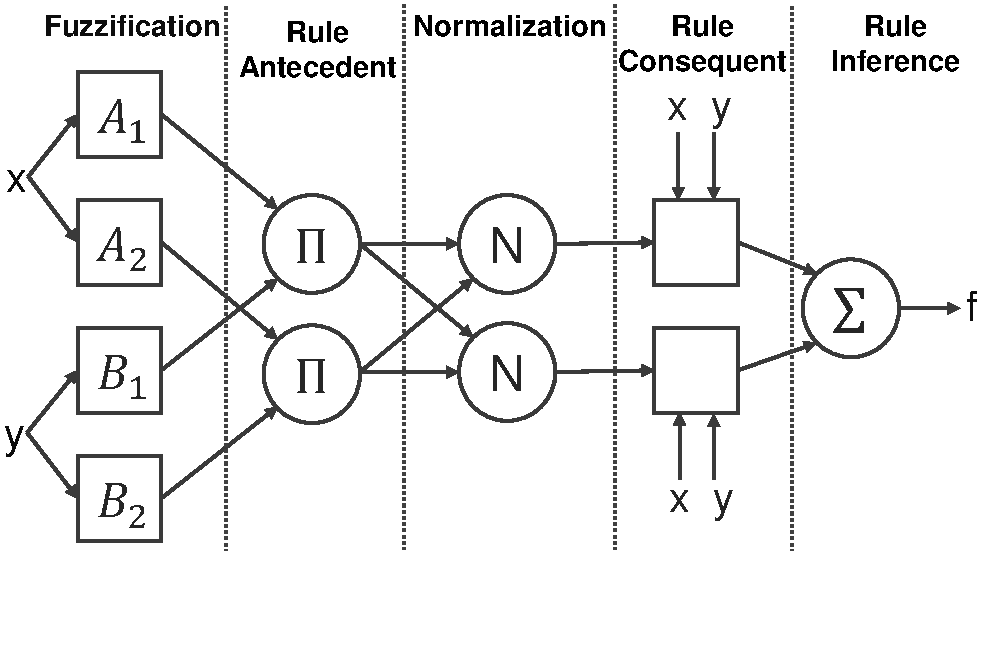
\includegraphics[width=\textwidth]{figs/Rory/ANFIS_diagram.pdf}
            \caption{}
            \label{fig:ANFIS_diagram}
          \end{subfigure}
          \hfill
          \begin{subfigure}[t]{0.48\textwidth} % Top-aligned subfigures
            \centering
            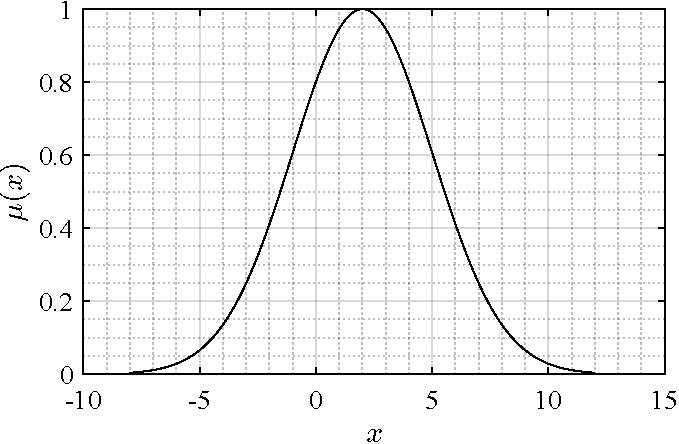
\includegraphics[width=\textwidth]{figs/Rory/mfs_plot.pdf}
            \caption{}
            \label{fig:membership_function_plot}
          \end{subfigure}
          \caption[ANFIS Network]{\textbf{a)} ANFIS network, with labelled layers. \textbf{b)} Gaussian membership function, with $c=2$ and $\sigma^2=9$.}
        \end{figure}

    
\subsection{ANFIS: Physics-Guided Fusion}

    \paragraph{Membership Functions}

        A fuzzy set is a linguistic representation of a numerical variable that has been fuzzified, enabling the modelling of uncertainty and partial truth. For example, the numerical range 1-10 can be categorised into the distinct fuzzy sets \textit{high, medium, low}. The value 9 would have a high \textit{degree of membership} in the fuzzy set \textit{high}, and a low degree of membership in the other sets. Membership functions are mathematical functions that assign each input value to a degree of membership \(\in [0,1]\) for each fuzzy set. 
        
        Gaussian membership functions have been chosen to represent the all of the environmental variables, and the sensor confidence values. The Gaussian membership function is defined as
        
        \[
        \mu(x) = \exp\left( -\frac{(x - c)^2}{2\sigma^2} \right),
        \]
        
        where \( c \) is the mode of the fuzzy set and \( \sigma^2 \) its variance, and is visualised in Figure \ref{fig:membership_function_plot}. This function is a smooth, differentiable bell curve.
        Gaussian membership functions are particularly well-suited for representing the natural variability in environmental parameters, such as soil moisture and ambient temperature, because many natural processes tend to be normally distributed, as suggested by the Central Limit Theorem \footnote{\url{https://en.wikipedia.org/wiki/Central_limit_theorem}}. Note that normalization is not necessary here because the membership values are degrees of activation rather than probability densities, and are scaled so that \(\mu(x)\in [0,1]\).
        
        In ANFIS, the network learns optimal \(c\) and \(\sigma\) parameters for each fuzzy set, tuning membership functions to best fit the fusion data. The Rule Antecedent layer determines the degree to which the fuzzy inputs satisfy the rules. The Rule Consequent layer decides the output of each rule. For Takagi-Sugeno Type-3 ANFIS \cite{jang1993anfis}, the Rule Consequents are learned as linear combinations of non-fuzzified inputs, and the outputs of all the rule consequents are combined to give a final fused confidence value. 

        
    \subsubsection{Fuzzy Rule Selection} \label{fuzzy_rules}
    

        ANFIS can be configured to include every possible 'rule' regarding the inputs to the network. However, this approach is computationally expensive, as the number of rules required scales as \((\textit{\#. fuzzy sets})^\text{(\textit{\#. inputs})}\). This makes this approach intractable when incorporating substantial domain knowledge (an example of this for time-series prediction is included in \cite{jang1993anfis}). Instead, it is more efficient to explicitly encode only the fuzzy rules that are expected to have the most significant impact, and is the approach taken here. These fuzzy rules are manually derived from the simulations in Sections \ref{compvis_thermalsims} and \ref{compvis_radarsims}, from first-principles physics, and general domain knowledge. The following rules are proposed for the ANFIS implementation:
        
        \begin{enumerate}

        
            \item \textbf{IF then soil moisture is high THEN thermal confidence is high.}\\

                \textbf{Justification:} As shown in Figure \ref{fig:conductivity}, the peak \(\Delta T\) increases with soil thermal conductivity. Given that soil thermal conductivity increases with soil water content \cite{wu2025soil}, and the \textbf{detectability hypothesis} in Section \ref{simulation_justification} argues that \(\Delta T\) can serve as a proxy for the detectability of a landmine viewed by the thermal sensor, it follows that higher soil moisture levels correlate with higher confidence in the thermal sensor.
            
            \item \textbf{IF soil moisture is high THEN radar confidence is low.}

                \textbf{Justification:} High soil moisture degrades radar performance by increasing the bulk soil electrical conductivity \cite{bai2013soils}, exponentially decreasing the penetration  depth\cite{giovanni2008penetration}, and thus reducing confidence in the radar sensor.

            \item \textbf{IF wind speed is high THEN thermal confidence is low}

                \textbf{Justification:} High wind speeds increase the rate of convective heat flux (Section \ref{compvis_thermalsims}) and tend to flatten soil surface temperature gradients, reducing \(\Delta T\) and thus reducing confidence in the thermal sensor.

            \item \textbf{IF soil is frozen THEN thermal confidence is low.}

                \textbf{Justification:} When the soil is frozen, any heat flow is absorbed by the latent heat of crystallisation, and temperature differences due to a landmine buried in the soil become undetectable. Therefore, thermal confidence is low when the soil is frozen.
 
        \end{enumerate}
        

        These rules are not exhaustive. If more domain knowledge becomes available, new fuzzy rules should be included to improve performance. To refine and expand the fuzzy rule database, an experimental campaign should be conducted to investigate the effects of additional environmental parameters on the sensor readings.

    
    \paragraph{Learning Approach of ANFIS}
    
        The ANFIS framework adopts a hybrid learning strategy that combines a feed-forward pass with backward error propagation. In the feed-forward phase, the fusion weightings (consequent parameters) are optimised with a least squares error (LSE) approach, whilst on the backwards pass, the membership function parameters (premise parameters) are optimised with gradient descent. This is described in Jang 1993 \cite{jang1993anfis}.
        
    
    By integrating physics-based constraints through fuzzy rules, and employing an adaptive learning strategy, ANFIS offers a fusion method that is both robust and interpretable. This approach is expected to outperform traditional methods by providing a solution grounded in the physical principles of sensor detection, as validated in Section \ref{compvis_anfisvalid}.
    
\subsection{ANFIS Validation} \label{compvis_anfisvalid}

Previous sections (Section \ref{fusion_bounds}) hypothesise that a physics-informed deep learning fusion network, such as ANFIS, will outperform a standard Naive Bayes (NB) fusion model. It is therefore important to validate this hypothesis with a (somewhat crude) simulation of environmental conditions and the \textbf{consequent} sensor data. This simulation aims to demonstrate that an ANFIS network with incorporated domain knowledge can improve data fusion performance over NB, when the sensor data are \textit{not} conditionally independent.

\subsubsection{Synthetic Data Generation}  
.
    ANFIS is expected to outperform NB because the latter assumes conditional independence between sensors, an assumption often invalid in real-world conditions where there is coupling between the two sensors through the causal physics of the environment. 
    
    To demonstrate NB's limitations, synthetic data is generated to model the influence of \textbf{soil moisture}. As detailed in Section \ref{fuzzy_rules}, increased soil moisture enhances thermal sensor return (via increased thermal conductivity) while inhibiting radar sensor return (via increased electrical conductivity). This is not the only coupling between the two sensors, but it suffices to model one to illustrate the advantages of ANFIS. Additionally, the model includes the effect of wind speed, which decreases thermal returns but does not affect radar returns.


    A 200$\times$200 grid was generated, with 2\% coverage of randomly placed mines. Soil moisture was simulated using a simplified sine-cosine function varying between 0 and 1, and is shown in Figure \ref{fig:anfis_summary}. Wind speed was modelled using random samples from a Gaussian distribution with a mean of 0 and a standard deviation of 2 (arbitrary units). Following the layered approach (Section \ref{layered_approach}), the radar sensor only samples points previously flagged by the thermal sensor. To simulate GPS drift and further illustrate the limitations of NB under uncertainty, a small random spatial shift was introduced between the thermal and radar datasets.


\subsubsection{Sensor Modelling}  

    The sensor confidence maps were computed using equations to model the effects of soil moisture (\textit{m}, dimensionless, ranging 0-1) and wind speed (\textit{w}, in \si{\metre\per\second}) on the thermal and radar sensor outputs. These curves are designed to reflect the higher precision characteristic of the radar sensor and the higher recall of the thermal sensor. Sensor noise was modelled as zero-mean Gaussian white noise ($\mathcal{N}$), with a variance of 0.15 for the thermal sensor, and 0.12 for the radar sensor. The resulting sensor output probabilities ($P$) are given by:
    
    \begin{equation}
        P_{\text{thermal}} = \begin{cases} 
        0.9 - 0.66e^{-m/40} - 0.02w + \mathcal{N}(0,0.15) & \text{if mine present} \\
        0.6 - 0.48e^{-m/200} - 0.02w + \mathcal{N}(0,0.15) & \text{if no mine}
        \end{cases}
    \end{equation}
    
    \begin{equation}
        P_{\text{radar}} = \begin{cases}
        1.2 \cdot 0.6e^{-m/60} + \mathcal{N}(0,0.12) & \text{if mine present} \\
        0.45 \cdot 0.6e^{-m/60} + \mathcal{N}(0,0.12) & \text{if no mine}
        \end{cases}
    \end{equation}

\subsubsection{Fusion Implementation}

    \paragraph{ANFIS} The ANFIS architecture is implemented using the Keras framework. The model accepts four input features: soil moisture, wind speed, thermal sensor confidence, and radar sensor confidence. Input fuzzification uses three Gaussian membership functions per input, whose parameters ($c,~\sigma$ in Equation \ref{eq:gaussian_mf}) are trainable variables within the network..

    While Section \ref{ANFIS} proposed explicit, physics-derived fuzzy rules, this implementation uses a \texttt{Dense} rule antecedent layer (see Figure \ref{fig:ANFIS_diagram}). A dense layer combines the membership degrees from the four inputs (each with 3 membership functions), allowing the network to learn the antecedent combinations corresponding to all $3^4=81$ possible fuzzy rules. The consequent layer learns the parameters that define the output for each of these implicitly formed rules. While traditional ANFIS employs a hybrid learning algorithm described in Section \ref{ANFIS}, this implementation utilizes standard backpropagation with the Adam optimizer for training efficiency within the Keras framework.
    
    The final custom output layer calculates a normalised, weighted sum of these rule outputs and applies a sigmoid function to ensure the final fused confidence is between 0 and 1.

    \paragraph{NB} The Naive Bayes (NB) fusion method combines the thermal and radar sensor confidence values $P_{\text{thermal}}$, $P_{\text{radar}}$. Assuming conditional independence between the sensors given the presence or absence of a mine, the fused confidence $P_{\text{fused}}$ is calculated using Bayes Theorem, which may be written as:

    \begin{equation}
        \label{eq:bayes_fusion}
        \mathcal{P}_\text{fused} = \frac{\mathcal{P}_\text{thermal}\mathcal{P}_\text{radar}}{\mathcal{P}_\text{thermal}\mathcal{P}_\text{radar} + (1-\mathcal{P}_\text{thermal})(1-\mathcal{P}_\text{radar})}
    \end{equation}
    
\subsubsection{Results and Conclusion}  

    The ANFIS model demonstrated improved recall (ANFIS: 0.66 NB: 0.11) and precision (ANFIS: 0.92 NB: 0.28), compared to Naive Bayes. The surprisingly low NB performance is partly caused by the random shifting between the radar the thermal maps, that means NB often gives null results from multiplying misaligned confidence values. However, more fundamentally, the simulation highlights ANFIS' key advantage; it can leverage the environmental context (soil moisture and wind speed inputs in this implementation) to implicitly model the physical coupling between sensor readings. Naive Bayes' inability to handle uncertainty and conditionally dependent data is also clear. See the predicted mine locations from each fusion algorithm in Figure \ref{fig:anfis_summary}.

     While this simulation is simplified, it validates the hypothesis that a deep learning fusion architecture, constrained to physically-plausible solutions and incorporates environmental context can perform significantly better than purely statistical methods, like Naive Bayes.

    \begin{figure}[h]
        \centering
        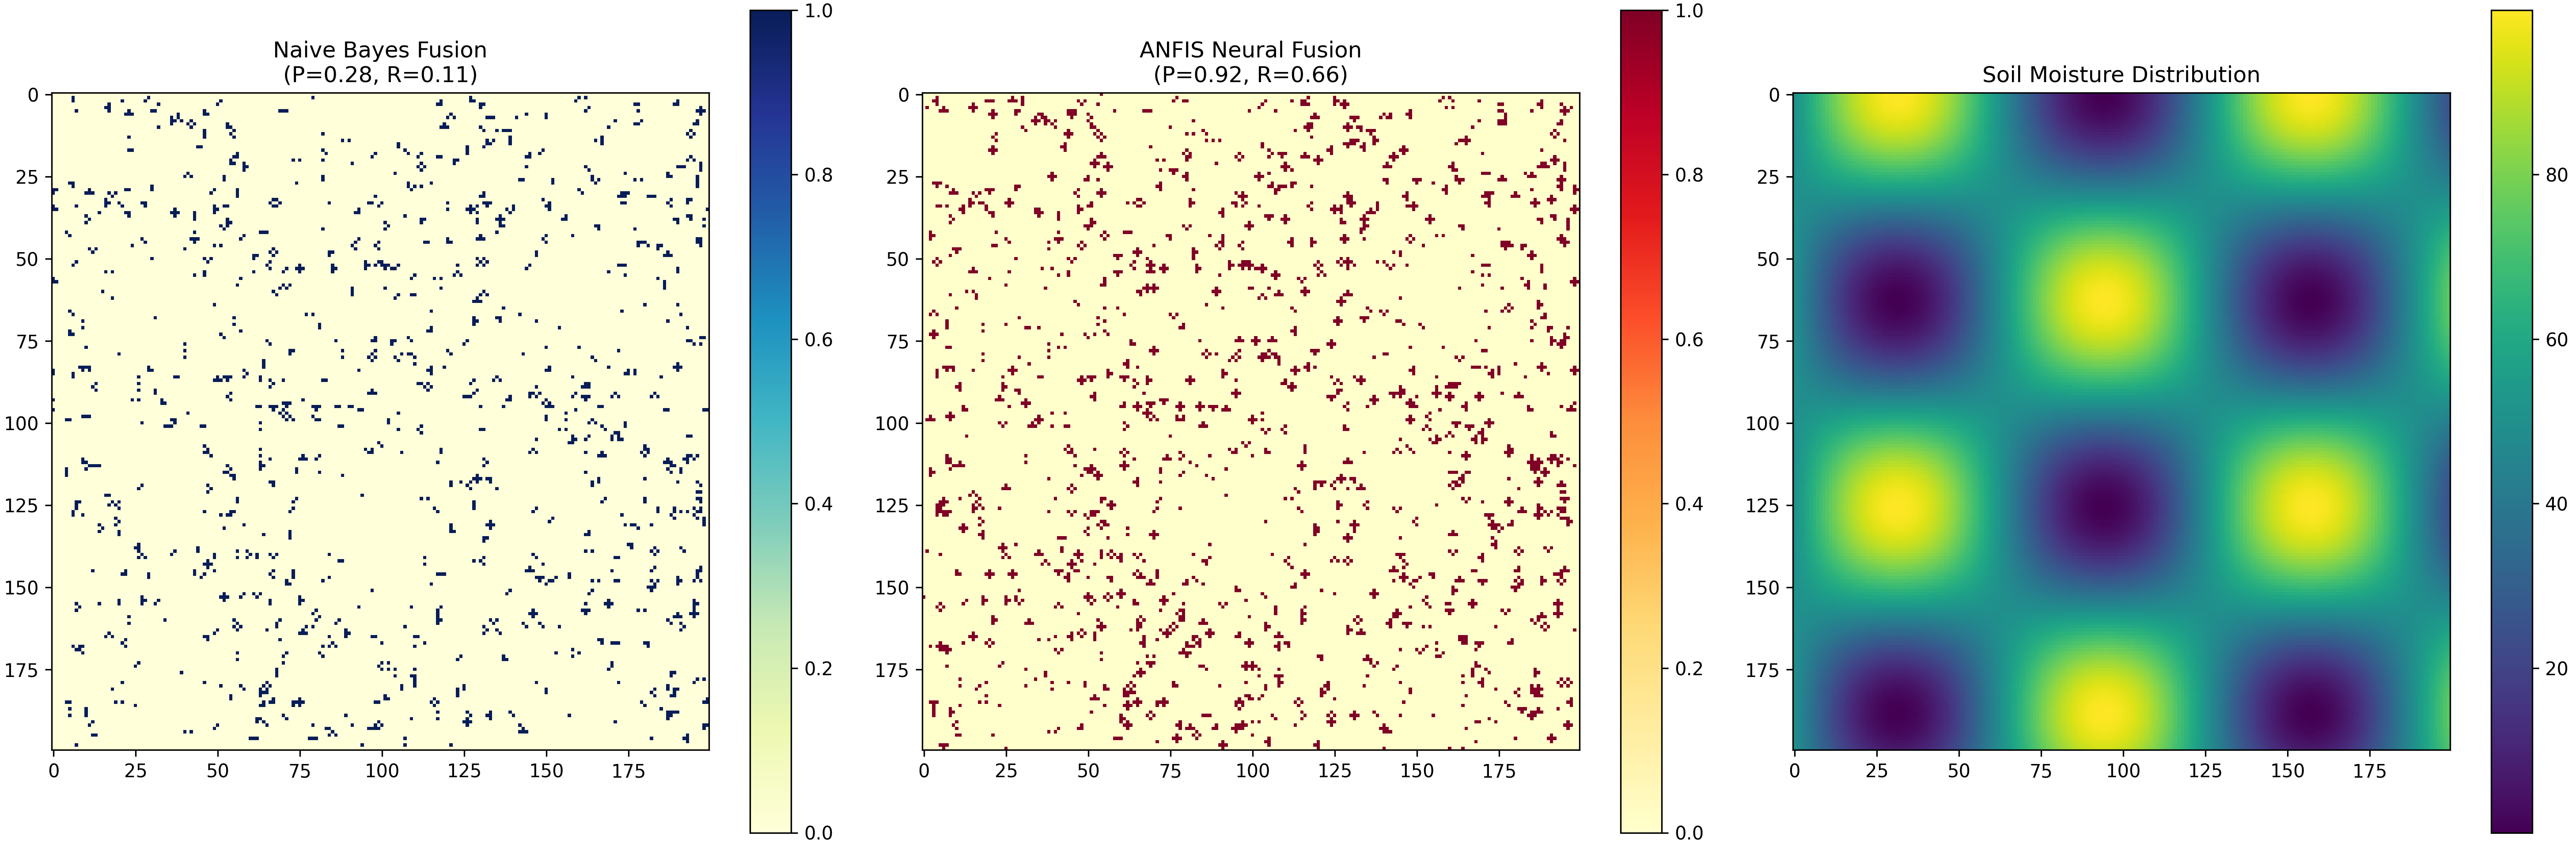
\includegraphics[width=0.98\textwidth]{figs/Rory/0_summary.png}
        \caption{ANFIS NB comparison summary. \textbf{Left:} simulated fusion for Naive Bayes. \textbf{Centre:} simulated fusion for ANFIS. \textbf{Right:} soil moisture distribution}
        \label{fig:anfis_summary}
    \end{figure}

    \paragraph{Future Work} 

        Several other physics-driven fusion algorithms exist. Another such approach is \textit{Physics Based Deep Learning} (PBDL)\footnote{\url{https://www.physicsbaseddeeplearning.org/intro.html}}, which benefits from implementing the physical domain knowledge at a deeper level in the \textit{model architecture and loss function}. PBDL is a recent field in Artificial Intelligence (AI), and it may have significant benefits, such as greater robustness to environmental variations in data-fusion for the detection of landmines.




%%%%
% \newacronym{LIPO}{LIPO}{lithium polymer}
% \newacronym{LIION}{Li-ion}{lithium-ion}
% \newacronym{gbp}{GBP}{Great British Pound}
% \newacronym{RESC}{RESC}{resonant switched capacitor}
% \newacronym{6s}{6s}{6-cell series}
% \newacronym{6s3p}{6s3p}{6-series 3-parallel}
% \newacronym{tim}{TIMS}{thermal interface materials}
% \newacronym{DCDC}{DC-DC}{Direct Current to Direct Current [power converter]
% }

% \newacronym{BS}{BS}{British Standards}
% \newacronym{ESR}{ESR}{equivalent series resistance}
% \newacronym{I2C}{I\textsuperscript{2}C}{Inter-Integrated Circuit }
% \newacronym{UART}{UART}{Universal Asynchronous Receiver/Transmitter }
% \newacronym{SRAM}{SRAM}{static random-access memory}
% \newacronym{SOC}{SOC}{state of charge}
% \newacronym{NTC}{NTC}{negative-temperature-coefficient}
% \newacronym{EKF}{EKF}{extended Kalman filter}
% \newacronym{FEM}{FEM}{finite element method}
% \newacronym{MOSFET}{MOSFET}{metal–oxide–semiconductor field-effect transistor}
%%%%

\fancyhead[C]{Samuel Grace}

\section{Battery Management System and Battery Hardware}
\label{sec:bms}
\subsection{Introduction and Motivation}

Although most drones do not contain one, an inbuilt \gls{BMS} \cite{SON2023120186} provides many key advantages when performing landmine detection. A \acrshort{BMS}, along with the corresponding bespoke circuit topology, supports the complex control system, high-quality sensor requirements and extended mission duration capabilities necessary for effective landmine detection. Additionally, it is possible to program a \acrshort{BMS} to optimise the battery cells’ lifespan; both reducing the operating cost and the environmental impact of the drone.

\subsection{Design and Component Selection}

Optimal design of the \acrshort{BMS} and the selection of appropriate components will determine the eventual success of the drone. It is necessary to choose components that will achieve the desired design solution, while balancing the considerations of cost, availability and sustainability.


\subsubsection{Cell Comparison and Selection}

The most important decision is selecting a battery cell chemistry. Drones typically use \gls{LIPO} batteries\footnote{\acrshort{LIPO} batteries are a subset of \acrshort{LIION} batteries. Conventionally, \acrshort{LIION} cells are taken to be those with a liquid electrolyte, whereas \acrshort{LIPO} cells have a polymer electrolyte.} due to their high maximum discharge current \cite{10808488}. However, following recent developments, \gls{LIION} batteries now have 30\% higher gravimetric energy density than \acrshort{LIPO} cells  \cite{Agrawal_2008}. Higher energy density permits longer flight times and carrying more sophisticated sensors, improving both the quality and quantity of the data gathered. \acrshort{LIION} cells are also more durable and safer than \acrshort{LIPO} cells, as they are more thermally stable and have a more rigid internal structure \cite{bergveld2014battery}. The decision matrix shown in Table \ref{tab:battery_comparison} compares different components based on set criteria to select the specific type of \acrshort{LIION} cell. The process involves weighting different factors according to their relative importance. The total energy of the cell is the most important factor, as it is directly proportional to the flight time and affects how much power is available for sensing. Weight is the next most significant factor since it affects both flight time and stability. Cost is the least important factor because the price of the cells is low compared to the price of other components of the drone. The scores for each factor are calculated by normalising relative to the \textit{best} of the three values and multiplying the normalised score by 10. The \textit{best} energy value is the highest, whereas the \textit{best} weight and the \textit{best} price values are the lowest. 

\begin{table}[h!]
\centering
\begin{tabular}{|l|c|c|c|c|}
\hline
\textbf{Specification} & 
\makecell{\textbf{Samsung}\\\textbf{3500mAh}\\\textbf{18650 Li-ion Cell}} &
\makecell{\textbf{Panasonic}\\\textbf{2040mAh}\\\textbf{18500NCR Li-ion Cell}} & 
\makecell{\textbf{Overlander}\\\textbf{4500mAh}\\\textbf{21700 Li-ion Cell}} & 
\textbf{Weighting} \\
\hline
\textbf{Energy (Wh)} & 12.95 & 7.55 & 16.65 & 60\%\\
\textbf{Energy Score} & 7.8& 4.5& 10.0& - \\\hline
\textbf{Weight (g)} & 48.5 & 33 & 70 & 30\% \\
\textbf{Weight Score} & 6.8& 10.0& 4.7& - \\
\hline
\textbf{Price \acrshort{GBP}} & 6.98 & 8.99 & 9.98& 10\%\\
\textbf{Price Score} & 10& 7.8& 7.0& - \\
\hline
\textbf{Total Score} & 7.7& 6.5& 8.1& 100\% \\
\hline
\end{tabular}
\caption[Battery Cell Comparison]{Comparison for energy capacity, weight, and price, with normalised scores and weighted totals.}
\label{tab:battery_comparison}
\end{table}

The \textbf{total score} \( S \) is calculated using Equation \ref{eq:score_formula}; all values used are taken from Overlander Batteries.\footnote{Overlander Batteries: \url{https://www.overlander.co.uk/}}

\begin{equation} \label{eq:score_formula}
S = w_C \times 10 \times\frac{\text{Energy}}{\text{Max. Energy}} + w_W \times 10 \times\frac{\text{Min. Weight}}{\text{Weight}} + w_P \times 10 \times\frac{\text{Min. Price}}{\text{Price}}
\end{equation}
\[(
\text{where }w_C, w_W, w_P \text{ are the importance weightings for capacity, weight and price respectively})
\]

From the results shown in Table \ref{tab:battery_comparison}, the design decision taken was to select the \textbf{Overlander 4500mAh 21700 Li-ion Cell}. Using \acrshort{LIION} cells improves reliability significantly because \acrshort{LIION} cells are much more durable than \acrshort{LIPO} cells due to their more rigid metal casing. Also, \acrshort{LIION} cells are less prone to thermal runaway, which reduces the risk of catastrophic failure when operating in hot, arid climates. Furthermore, \acrshort{LIION} cells are more environmentally sustainable than \acrshort{LIPO} cells because they have a longer average lifetime and higher recyclability.

However, there are important sustainability considerations regarding the \acrshort{LIION} cells, such as the vast quantities of energy required in the production process \cite{environments12010024}. It is also important to ensure that the lithium mining process used to source the material for the battery is conducted in both an environmentally and ethically sustainable way \cite{EnergyFuturesLab_2022}. 

\textbf{Overlander}, the chosen supplier for the batteries, has detailed policies about their compliance in all of these areas, which guarantees that the cells used are sustainable. The custom design of the \gls{BMS} ensures that cell balancing, charging and discharging strategies are optimised to maximise battery life and durability. This optimisation further improves the sustainability by reducing the frequency at which the \acrshort{LIION} cells must be replaced. 

\subsubsection{Microcontroller, Charger and Sensor Selection}
\label{microcon}

The \acrshort{BMS} requires a microcontroller with sufficient processing power to perform the state estimations using Kalman filters and to run the algorithms controlling the battery cells. The device used must also be able to communicate with sensors and other devices using \gls{I2C} and \gls{UART} protocols \cite{Denggao2022}. Accordingly, the \textbf{STM32F405} microcontroller was selected. It offers a clock speed of 168 MHz, 192 Kbytes of \gls{SRAM} and 512 Kbytes of flash memory \cite{st_dm00037051}. These performance metrics mean that the \textbf{STM32F405} is sufficiently powerful to compute accurately the state estimations and run the \acrshort{BMS} algorithms. \textbf{iMAX B6 V2 Chargers} were selected, allowing for quick and efficient charging between missions \cite{digikey_prt16793}.

A variety of measurements are required to provide the \acrshort{BMS} with the required data to estimate the \gls{SOC} of the cells. First, the \textbf{TI BQ76972} sensors provide accurate cell voltage measurements and communicate using the \acrshort{I2C} interface. The \textbf{TI BQ769142} battery monitor provides measurements of the battery current, and also communicates using the \acrshort{I2C} protocol. An advantage of using the \textbf{TI BQ769142} is that it additionally supports temperature sensing using \gls{NTC} thermistors positioned inside the battery pack; the thermistors are used to provide accurate measurements for each cell within the battery cell stack. Texas Instruments provided the methodology that was followed \cite{TI_SNIA032}, specifically for use within a \gls{BMS}.

\subsubsection{Kalman Filtering Techniques}
\label{kalm}

Kalman filters are implemented on the \textbf{STM32F405} microcontroller to estimate the various states in the battery, such as temperatures, voltages and currents. The Kalman filter's purpose is to estimate the states using indirect, uncertain measurements \cite{kalfilt}. 

For each state, the underlying physical process is modelled in state-space form, and the system is discretised to allow a Kalman filter to be implemented in C using a Kalman filtering library designed for embedded systems \cite{computers11110165}. As an example of the process, the estimation of the \gls{SOC} using an \gls{EKF} was simulated. The \gls{EKF} algorithm is explained in detail by \cite{kalfilt}.  The \gls{SOC} is defined by Equation \ref{eq:soc}, where $C$ represents the battery's capacity.

\begin{equation}
\label{eq:soc}
\text{SOC (\%)} = 100 \times \frac{C_{\text{releasable}}}{C_{\text{rated}}}
\end{equation}

For the \gls{SOC} measurement, an \gls{EKF} is used in conjunction with the Coulomb counting method to estimate the \gls{SOC}. The \gls{EKF} was chosen over other methods, such as using a particle filter, since the \gls{EKF} is significantly less computationally intensive when working with few states, as is the case here \cite{STELZER20171483}. The \gls{EKF} accounts for measurement noise, which allows the \gls{EKF} to produce a high-fidelity estimate of the \gls{SOC} variation \cite{Zaki2025}.

 The simulation for the \gls{SOC} estimation process was performed using the Simscape Battery Toolbox, by adapting an existing model template.\footnote{\url{https://mathworks.com/help/simscape-battery/ug/estimate-battery-soc-using-kalman-filter-example.html}} The results are shown in Figure \ref{fig:bmsestimefk}, with Figure \ref{fig:coolomb} showing the estimate produced solely using the state-space model of the process. The residual error is clearly visible when relying solely on the state-space model, which suggests that a more sophisticated approach is required. Figure \ref{fig:kalmeff} shows the results of applying the \gls{EKF}, which successfully removes the offset that is visible in Figure \ref{fig:coolomb}.


\begin{figure}[H]
    \centering
    \begin{subfigure}[b]{0.49\textwidth} % Use [b] to align captions at the bottom
        \centering
        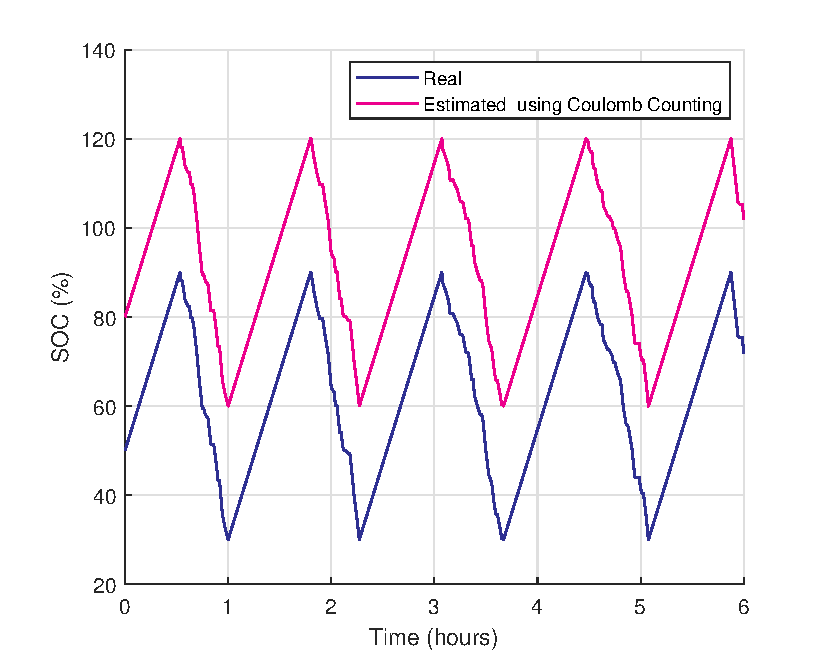
\includegraphics[width=\textwidth]{figs/Samuel/Figures/plotsbattest (1) (cropped) (pdfresizer.com).pdf}
        \caption{Estimate using Coulomb counting.}
        \label{fig:coolomb}
    \end{subfigure}
    \hspace{0\textwidth}
    \begin{subfigure}[b]{0.49\textwidth} % Use [b] to align captions at the bottom
        \centering
        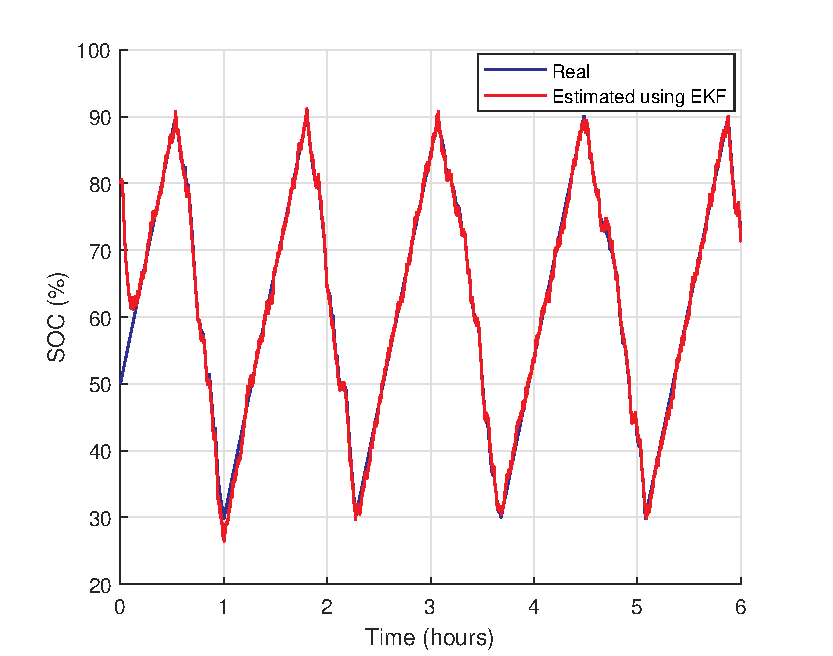
\includegraphics[width=\textwidth]{figs/Samuel/Figures/plotsbattest (1) (cropped) (pdfresizer.com) (1).pdf}
        \caption{Estimate additionally using \gls{EKF}.}
        \label{fig:kalmeff}
    \end{subfigure}
    \caption[Comparison of State of Charge Estimates]{Comparison of State of Charge estimates using the Simscape Kalman Filter Template}
    \label{fig:bmsestimefk}
\end{figure}

\subsection{Internal System}

The overall structure of the \acrshort{BMS} is shown in Figure \ref{fig:bms_layout}, adapted from \cite{7555475}. For clarity, the battery pack depicts one set of the \acrshort{6S} cells. In reality, the system has a \acrshort{6S3P} configuration of cells. Sensor information from each cell in the battery pack is transmitted to the State Estimator, where Kalman filtering techniques are used to infer the states from the measurements. The State Estimator, including the \gls{EKF}, was incorporated into the model in MATLAB and Simulink utilising the Simscape Battery Toolbox.

The Master Control Unit represents the \textbf{STM32F405} microcontroller chosen in Section \ref{microcon}. The microcontroller implements the \gls{RESC} switching techniques detailed in Section \ref{swit}, as depicted by the \textbf{Cell Equalisation} component of the BMS.

\begin{figure}[H]
  \centering
  \vspace{5mm}
  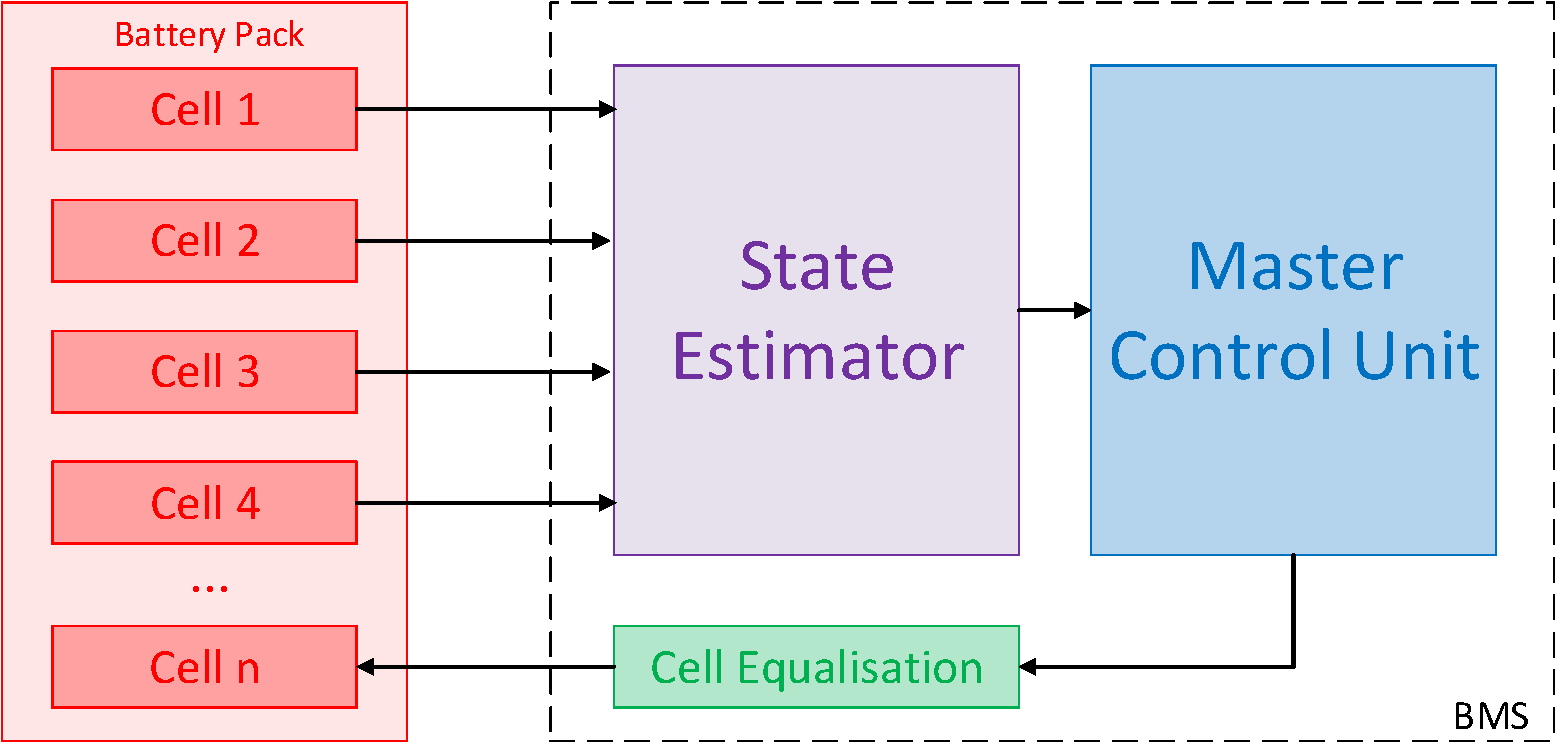
\includegraphics[width=0.75\textwidth]{figs/Samuel/Figures/BMS Internal (1)-cropped.pdf}
  \caption[Battery Management System Layout]{Battery Management System Layout adapted from \cite{7555475}}
  \label{fig:bms_layout}
  \vspace{5mm}
\end{figure}






\subsubsection{Battery Cell Stack Configuration}

A simplified diagram of the cell switching layout used is shown in Figure \ref{fig:bcs}. The switching topology used is the \gls{RESC} layout. For conciseness, Figure \ref{fig:bcs} shows a simplified \gls{6S} circuit. In reality, a \gls{6S3P} layout is used, but this change does not affect the principles of operation. 

The use of capacitors, inductors and resistors allows for reduced equalisation time and less energy loss compared to simpler switched-capacitor methods \cite{8467638}. The core ideas and theory used to develop the \gls{RESC} layout shown in Figure \ref{fig:bcs} are discussed in \cite{8681672}, and additional simulation and modelling are utilised to verify the configuration's applicability in this context.

\begin{figure}[H]
\centering
\vspace{10mm}
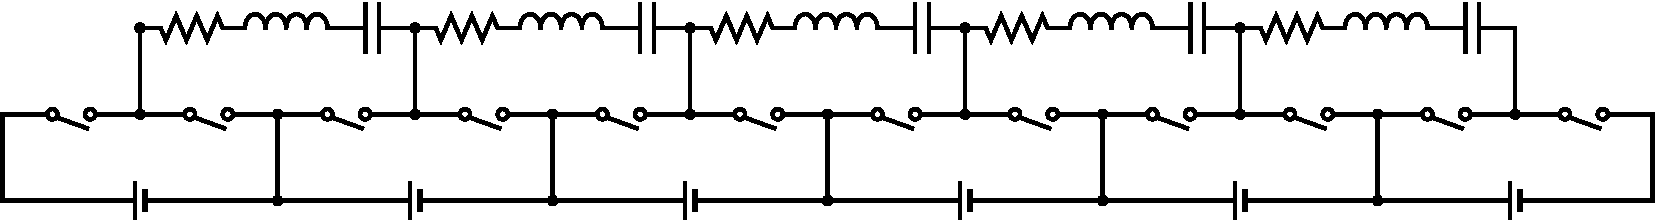
\includegraphics[width=0.99\textwidth]{figs/Samuel/Figures/resc1-cropped.pdf}
\caption[Simplified Battery Cell Stack Configuration]{Simplified battery cell stack configuration, adapted from \cite{8467638}}
\label{fig:bcs}
\end{figure}

\subsubsection{Cell Switching Simulations}
\label{swit}

The \gls{RESC} switching technique outlined in \cite{8467638} was implemented in MATLAB, and the results obtained are shown in Figure \ref{fig:resccrop}. The methodology involved initialising each battery voltage with a random value between 3 V and 4 V and then performing the equalisation strategy. Figure \ref{fig:reccrop} shows the results obtained when using a simpler switched capacitor equalisation strategy. By contrasting the two plots shown in Figure \ref{fig:rescvrec}, the improved equalisation time given by the \gls{RESC} strategy can be observed. 

The results produced by the simulation are consistent with results from similar models \cite{8467638}, albeit for cells with significantly different parameters. The moderate differences in cell voltages model a situation where a cell is damaged or unusable, and due to the cell stack configuration, normal operation can be quickly resumed by equalising the remaining cells.

\begin{figure}[H]
    \centering
    \vspace{5mm}
    \begin{subfigure}[b]{0.4\textwidth} % Use [b] to align captions at the bottom
        \centering
        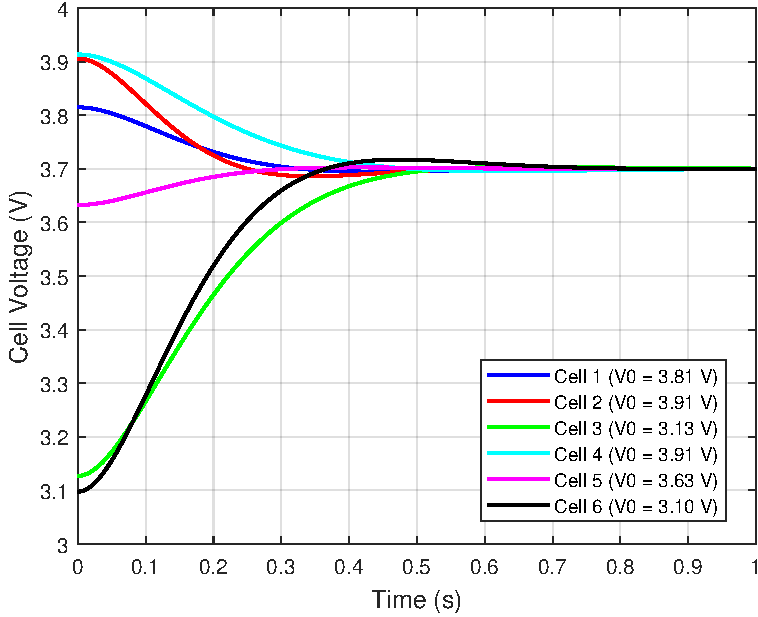
\includegraphics[width=\textwidth]{figs/Samuel/Figures/cellV-cropped.pdf}
        \caption{\gls{RESC} switching strategy}
        \label{fig:resccrop}
    \end{subfigure}
    \hspace{0.07\textwidth}
    \begin{subfigure}[b]{0.388\textwidth} % Use [b] to align captions at the bottom
        \centering
        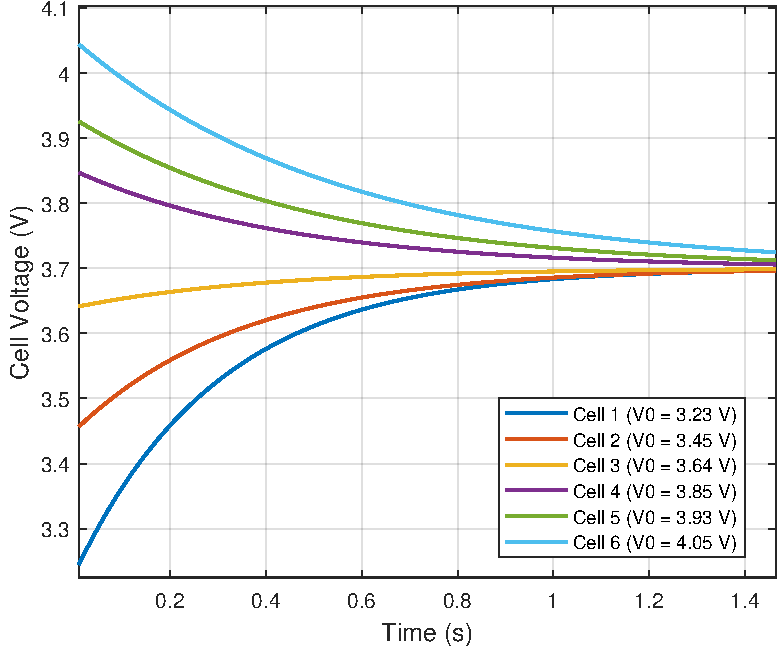
\includegraphics[width=\textwidth]{figs/Samuel/Figures/recpdf-cropped.pdf}
        \caption{Simpler switched-capacitor strategy}
        \label{fig:reccrop}
    \end{subfigure}
    \caption[Comparison of Cell Equalisation Strategies]{Comparison of cell equalisation strategies using the method outlined in \cite{8467638}}
    \label{fig:rescvrec}
\end{figure}

\subsubsection{Thermal Management Design and Simulations}

Designing an efficient thermal management system has numerous advantages for battery operation, with the most significant benefit being the ability to extend the cells' lifetimes by 30-50\% \cite{TOGUN20251077}. The design used in this \gls{BMS} focuses on utilising passive cooling techniques to regulate and balance the battery's temperature. Specifically, \gls{TIMS} are used to regulate the transfer of heat between individual cells and their surroundings. In this design, a thin thermally conductive layer is inserted between the cells to aid heat dissipation. This passive cooling measure is especially useful when there are many cells, ensuring that even if some cells generate more heat, the overall temperature distribution remains balanced. Figure \ref{fig:tempythings} shows how temperature influences the discharge time (Figure \ref{fig:tempy1} from Chen, 2013 \cite{chen2013heat}) and the cycle life (Figure \ref{fig:tempy2} from \cite{REZVANIZANIANI2014110}). These graphs illustrate the importance of effective thermal management. Maintaining an operating temperature within the 20$^\circ\text{C}$ to 45$^\circ\text{C}$ range prevents the cell from discharging too rapidly and maximises the cycle life.

\begin{figure}[H]
    \centering
    \begin{subfigure}[b]{0.47\textwidth} % Use [b] to align captions at the bottom
        \centering
        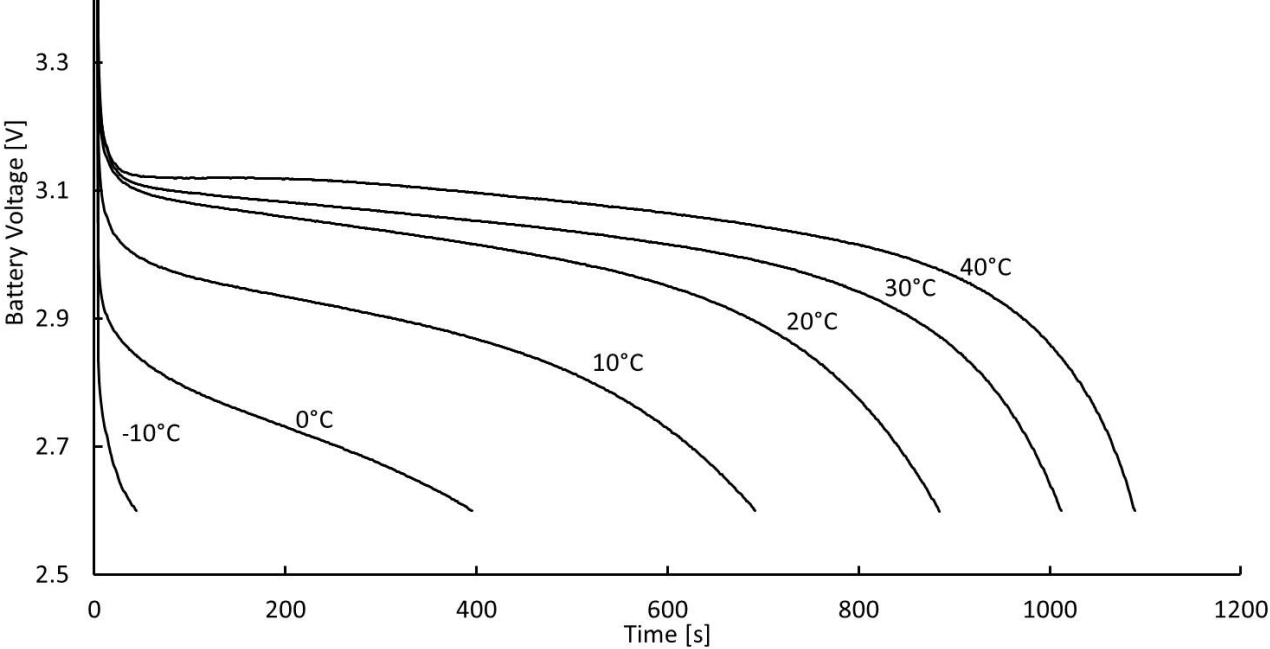
\includegraphics[width=\textwidth]{figs/Samuel/Figures/chenbattery.png}
        \caption{Cell voltage vs. time \cite{chen2013heat}}
        \label{fig:tempy1}
    \end{subfigure}
    \hspace{0.04\textwidth}
    \begin{subfigure}[b]{0.47
    \textwidth} % Use [b] to align captions at the bottom
        \centering
        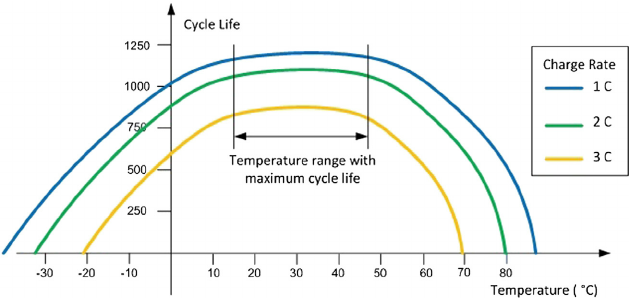
\includegraphics[width=\textwidth]{figs/Samuel/Figures/Lithium-ion-battery-life-vs-temperature-and-charging-rate-36-39-44-45.png}
        \caption{Variation of cycle life vs. temperature \cite{REZVANIZANIANI2014110}}
        \label{fig:tempy2}
    \end{subfigure}
    \caption[Effects of Temperature Variation on Cell Properties]{Effects of temperature variation on cell properties, figures from \cite{chen2013heat} (a) and \cite{REZVANIZANIANI2014110} (b).}
    \label{fig:tempythings}
\end{figure}

Using the Simulink and Simscape software, a high-fidelity model of the cells with the passive thermal management system was constructed. Cooling analysis of the battery was performed using simulation data, allowing for the use of realistic heat fluxes. The cell geometries were modelled, and the \gls{FEM} was utilised to analyse the heat evolution over time by adapting an existing Simulink template.\footnote{\hyperlink{https://mathworks.com/help/pde/ug/battery-module-cooling-analysis-and-reduced-order-thermal-model.html}{mathworks.com/help/pde/ug/battery-module-cooling-analysis-and-reduced-order-thermal-model.html}} To provide meaningful results, the thermal analysis was run in parallel with the simulation example performed in Section \ref{mocs}. The battery temperature data shown in Figure \ref{fig:battemp} is an average of all 18 cells' temperatures for Agent 2 in the simulation. The graph shows that the temperature remains within the optimal temperature regime for the duration of the mission, indicating that the passive thermal management approach is sufficient to maximise cell performance and cycle life.

\begin{figure}[H]
\centering
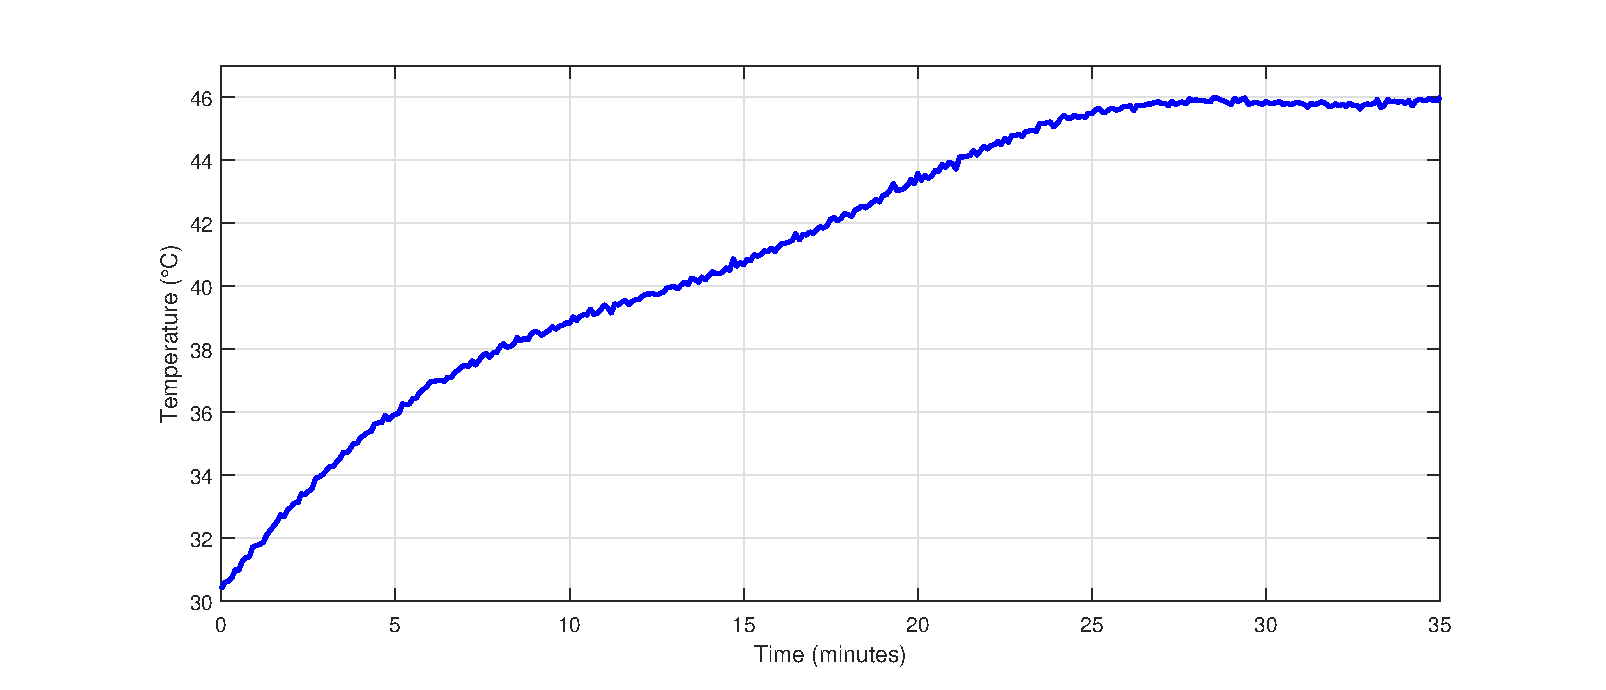
\includegraphics[width=0.73\textwidth]{figs/Samuel/Figures/batttemp.eps}
\caption{Battery temperature for Agent 2 in Section \ref{simdata}}
\label{fig:battemp}
\end{figure}

\subsection{DC-DC Converter Design}

A \acrshort{DCDC} converter is an integral part of the interface between the drone's battery management system and the rest of the \acrshort{UAV}'s circuitry. It allows for the conversion of the cells' combined output voltage into a voltage which can be used in the drone's motors and control unit. Despite linear voltage regulation being a much simpler approach, switched-mode \acrshort{DCDC} converters are considered here because switched-mode converters have a much higher efficiency than linear regulators \cite{rogers2024powerelectronics}. As a result, fewer cells are required, thus reducing the drone's weight.

\subsubsection{Circuit Topology Selection}

Numerous switched-mode converter topologies exist, with the most common types being the Buck, Boost and Buck-Boost converters. For this application, however, a \textbf{non-isolated Ćuk converter} will be used. The crucial advantage gained by using a non-isolated Ćuk converter is the significantly reduced current ripple it exhibits compared to the other switched-mode converters mentioned \cite{cuk1981dc-to-dc}. The low current ripple minimises electrical noise within the circuit, which is important for ensuring that the data generated by the sensors is accurate. Another advantage of the Ćuk converter is that since there is continuous power transfer via the capacitor, electromagnetic interference is minimised, again helping to maximise the accuracy of the sensors. The most significant issue involved with using a Ćuk converter is the large voltage stress on the transistor \cite{Bailey:1641409}. This problem can be mitigated by selecting a \gls{MOSFET} switch with a high voltage rating. In this instance, the battery's maximum output voltage is 25 V, so a \gls{MOSFET} rated at 60 V gives an acceptable safety margin.

\subsubsection{Component Selection}

The Ćuk converter produces an inverted voltage output, so the corresponding circuitry must be carefully designed to account for the reversed polarity to ensure that the voltage does not require further inversion. Equation \ref{eq:cuk} gives the output voltage $V_{OUT}$ in terms of the input voltage $V_{IN}$ and the duty cycle $D$.

\begin{equation}
  \frac{V_{OUT}}{V_{IN}} = - \frac{D}{1-D}
  \label{eq:cuk}
\end{equation}

The layout of the non-isolated Ćuk converter circuit is shown in Figure \ref{fig:cukdiagram}.

\begin{figure}[H]
  \centering
  \includegraphics[width=0.68\textwidth]{figs/Samuel/Figures/mosfet cuk (1).pdf}
  \caption{Ćuk Converter Circuit Topology}
  \label{fig:cukdiagram}
\end{figure}



The switch S\textsubscript{1} in Figure \ref{fig:cukdiagram} operates at a \textbf{low switching frequency} $f_{sw} =$ 100 kHz. Using this low frequency minimises the potential for electromagnetic interference. The switching of the \acrshort{MOSFET} is controlled by a gate driver. The diode D\textsubscript{1} shown in Figure \ref{eq:cuk} is a \textbf{Schottky diode}, which is designed for faster switching rates than a silicon p-n diode \cite{Schottky}. The battery will initially output 25 V when fully charged, with this decreasing to 18 V when the battery is in its discharged state. The passive component values for the Ćuk converter are determined by assuming that $V_{IN}$ = 21.5 V, which is the midpoint of the battery's output voltage range. The input and output current ripple must be sufficiently small to minimise noise, so the peak-to-peak inductor ripple currents $\Delta I_{L1}$ and $\Delta I_{L2}$ must satisfy $\Delta I_{L_{i}} \approx 0.1$ A,$\quad \text{for } i = 1, 2$. Also, the peak-to-peak output voltage ripple, $\Delta V_{OUT}$, should be approximately equal to 0.1\% of the output voltage, so for a 5 V output rail,  $\Delta V_{OUT} \approx $ 5 mV is required. The approximate output ripple currents and output voltage ripple are given by Equations \ref{eq:iL} and \ref{eq:Vo}, respectively \cite{EricksonRobertW2020FoPE}.

\begin{equation}
\Delta I_{L_{i}} \approx \frac{ V_{IN} D}{ f_{sw} L_i}, \quad \text{for } i = 1, 2
\label{eq:iL}
\end{equation}

\begin{equation}
\Delta V_{OUT} \approx \frac{V_{OUT} (1 - D)}{8C_2 L_2 (f_{sw})^2}
\label{eq:Vo}
\end{equation}


Equation \ref{eq:cuk} gives a duty cycle of $D \approx$ 0.19 for the given $V_{IN}$ and $V_{OUT}$ voltages. Using this duty cycle and rearranging Equation \ref{eq:iL} gives L\textsubscript{1} $\approx$ 400 $\mu$H and L\textsubscript{2} $\approx$ 400 $\mu$H, since both inductors have the same maximum current ripple. Rearranging Equation \ref{eq:Vo} gives C\textsubscript{2} $\approx$ 20 $\mu$F, which ensures that $V_{OUT}$ is smooth. C\textsubscript{1} $\approx$ 40 $\mu$F is selected to balance the benefits of a low equivalent series resistance with the added smoothness gained from a higher capacitance value.  The component values are chosen from the \acrshort{BS} 2488 E24 series preferred values \cite{HLT}, so: C\textsubscript{1} $=$ 43 $\mu$F, L\textsubscript{1} $=$ 390 $\mu$H, C\textsubscript{2} $=$ 20 $\mu$F and  L\textsubscript{2} $=$ 390 $\mu$H. 

\subsubsection{Circuit Simulation}

The Ćuk converter is accurately modelled in a simulation environment to verify the expected behaviour of the \acrshort{DCDC} converter over the range of $V_{IN}$ values supplied from the battery management system. The Simscape Electrical Ćuk converter template from MathWorks is used to implement the model of the circuit, using the ode23tb differential equation solver to compute the voltage and current evolutions over time. The ode23tb equation solver is an implicit Runge-Kutta method \cite{matlab_ode23tb}, which is able to solve the Ćuk converter equations both rapidly and accurately.

Modelling the \gls{ESR} of each component is an important aspect of the simulation since the \acrshort{ESR} has a significant impact on the output voltage ripple $\Delta V_{OUT}$ and output current ripple $\Delta I_{OUT}$. The Simscape Electrical software can model the \acrshort{ESR}, so the numerical values for the \acrshort{ESR} of the components were included in the simulation. To validate the theoretical output voltage ripple and current ripple across all of the possible battery output voltages, the simulation was run for input voltage values at 1 V intervals within the operating range of the battery, $V_{IN}$ = 18 V to $V_{IN}$ = 25.2 V. The results of these simulations are shown in Table \ref{tab:converter_performance}.

\begin{table}[h]
    \centering
    \renewcommand{\arraystretch}{1.2}
    \begin{tabular}{cccc}
        \toprule
        $V_{IN}$ (V) & $\Delta V_{OUT}$ (mV) & $\Delta I_{OUT}$ (A) & $D$ \\
        \midrule
        18.0 & 5.27 & 0.100 & 0.217 \\
        19.0 & 5.13 & 0.098 & 0.208 \\
        20.0 & 5.41 & 0.103 & 0.200 \\
        21.0 & 5.63 & 0.103 & 0.192 \\
        22.0 & 5.52 & 0.105 & 0.185 \\
        23.0 & 5.53 & 0.102 & 0.179 \\
        24.0 & 5.63 & 0.105 & 0.172 \\
        25.0 & 5.67 & 0.106 & 0.167 \\
        25.2 & 5.63 & 0.106 & 0.166 \\
        \bottomrule
    \end{tabular}
    \caption{Output Ripple Characteristics and Duty Cycle Relationship}
    \label{tab:converter_performance}
\end{table}


 The results conform with the theoretical expectations, in most cases having similar numerical values to those predicted by Equations \ref{eq:iL} and \ref{eq:Vo}. Any discrepancies from the predicted values are likely due to second-order effects included in the simulation that Equations \ref{eq:iL} and \ref{eq:Vo} do not model. The simulation shows that the output voltage ripple and current ripple are well within the acceptable range for low-noise applications. Therefore, the Ćuk converter can safely be deployed as part of the \acrshort{BMS} circuitry onboard the drone, with minimal electromagnetic interference.


For each of the voltages tested in Table \ref{tab:converter_performance} above, two plots of the output voltage $V_{OUT}$ and output current $I_{OUT}$ were generated. As an example, the results produced with $V_{IN}$ = 22 V are shown in Figure \ref{fig:cukmatlab}. In each of the plots, the average value is shown by a black dashed line, and labelled vertical lines denote the \textit{peak-to-peak} voltage and current ripple on the waveforms in Figures \ref{fig:cukmatlab_a} and \ref{fig:cukmatlab_b}, respectively. 

\begin{figure}[H]
\centering
\subfloat[Plot of the steady-state output voltage $V_{OUT}$]{
    \includegraphics[width=\textwidth]{figs/Samuel/Figures/CukPlots (cropped) (pdfresizer.com).pdf}
    \label{fig:cukmatlab_a}
}

\vspace{0.1cm} % Add vertical space between subfigures (adjust as needed)

\subfloat[Plot of the steady-state output current $I_{OUT}$]{
    \includegraphics[width=\textwidth]{figs/Samuel/Figures/CukPlots (cropped) (pdfresizer.com) (1).pdf}
    \label{fig:cukmatlab_b}
}
\caption{Simscape simulation results for the Ćuk converter}
\label{fig:cukmatlab}
\end{figure}

\subsection{Overall Circuit Layout}

A high-fidelity simulation of the \gls{BMS} was constructed using MATLAB, Simulink and Simscape. This model was then integrated into the overall system to allow the multi-agent system to be modelled using the designed \gls{BMS}; the results obtained are shown in Section \ref{mocs}. Figure \ref{fig:bms_ovrlayout} shows a simplified version of the \gls{BMS} location within the drone's circuitry, as modelled in the simulation.

\begin{figure}[H]
  \centering
  \includegraphics[width=0.79\textwidth]{figs/Samuel/Figures/BMS-cropped.pdf}
  \caption{Overall circuitry layout}
  \label{fig:bms_ovrlayout}
\end{figure}


\usetikzlibrary{shapes.geometric, arrows}

\tikzstyle{startstop} = [rectangle, rounded corners, 
minimum width=3cm, 
minimum height=1cm,
text centered, 
draw=black, 
fill=red!30]

\tikzstyle{io} = [trapezium, 
trapezium stretches=true, % A later addition
trapezium left angle=70, 
trapezium right angle=110, 
minimum width=3cm, 
minimum height=1cm, text centered, 
draw=black, fill=blue!30]

\tikzstyle{process} = [rectangle, 
minimum width=3cm, 
minimum height=1cm, 
text centered, 
text width=3cm, 
draw=black, 
fill=orange!30]

\tikzstyle{decision} = [diamond, 
minimum width=3cm, 
minimum height=1cm, 
text centered, 
draw=black, 
fill=green!30]
\tikzstyle{arrow} = [thick,->,>=stealth]

%%
% \newacronym{cad}{CAD}{computer-aided design}
% \newacronym{pid}{PID}{proportional–integral–derivative}
% \newacronym{dnn}{DNN}{Deep Neural Network}
% \newacronym{lqr}{LQR}{linear-quadratic regulator}
% \newacronym{mpc}{MPC}{model predictive control}
% \newacronym{pd}{PD}{proportional–derivative}
%%

\fancyhead[C]{Samuel Grace}

\section{Simulation and Control}
\label{sec:simcontrol}

\subsection{Introduction and Overview}

In this section of the project, software was developed to simulate the multi-agent aerial robotic system. For a drone to be able to capture useful images, it is essential that the drone can hover with minimal disturbance to its position. Achieving this stability requires a controller that is robust to sensor noise and environmental disturbances. The development of the flight control system focused on ensuring that the \gls{uav} was sufficiently stable during a period of hovering while also making the controller suitable for general flight.

A \gls{bms} was designed to optimise the drone's performance, further extending the mission duration as well as providing the other advantages discussed in Section \ref{sec:bms}. By combining the bespoke controller with the customised \gls{bms} components, the performance of the \gls{uav} was enhanced, making it ideal for detecting landmines in a wide range of environmental conditions.

The results obtained in this section were generated solely from simulations run within the C, Python, MATLAB, Simulink and Simscape environments. These simulations provided insights into the operation of the drone using a cascade \gls{pid} controller designed specifically for the chosen mission.  

Real-time environmental conditions were also modelled in the simulations. The controller is designed to be implemented onboard the drone using embedded C. The details of the hardware and software used to perform these simulations are outlined in Table \ref{tab:computersetup}. The ARM GNU Toolchain is used to test the C code developed for use onboard the drone.  
\begin{table}[h]
\vspace{5mm}
\begin{center}
\begin{tabular}{| p{6cm}|p{10cm}|}
 \hline
 \textbf{Specification}       & Details\\ 
 \hline
 Computer Model                & HP ENVY Laptop - 17-cg0002na          \\ 
 CPU Type                     & Intel Core i7-1065G7 with 4 cores, up to 3.90 GHz \\ 
 Operating System and Version & Windows 11 Home, Version 23H2, OS Build 22631.4460 \\ 
 Memory (RAM)                 & 16 GB DDR4-3200 SDRAM (2x8GB)      \\  
 Storage                      & HP 512GB PCIe NVMe M.2 SSD            \\ 
 MATLAB Version               & 24.2.0.2712019 (R2024b) \\
 Control Loop Frequency&400 Hz\\ 
  Python Version& Python 3.12.1\\
 C Version&C17 (ISO/IEC 9899:2018)\\ 
 GNU Toolchain& ARM GNU Toolchain 12.3.Rel1 (for STM32H7)\\ 
 \hline
\end{tabular}
\end{center}
\caption{Computer Hardware and Software Specifications}
\label{tab:computersetup}
\end{table}

Figure \ref{fig:simctrloverview} shows the overall scheme of the simulation and control process. First, the location coordinates were passed into the software to enable environmental, weather and climate effects to be accurately modelled. Next, the \gls{cad} model of the drone was analysed to represent the drone's dynamics within the simulation.

An iterative simulation and refinement process was used to determine the required parameters for the cascade \gls{pid} controller used. These steps made use of the Meteomatics API to provide accurate weather data, as explained in Section \ref{gust}. Deployment of the optimised controller was then simulated in conjunction with the \gls{bms} to ensure that the drone had adequate battery capacity for the planned mission. 

Once a single drone had been modelled, the simulation was then extended to model the multi-agent operation in the presence of motor nonidealities and environmental disturbances. The increased complexity introduced by this approach was worthwhile since it provided additional confidence that each agent could carry out their mission while maintaining a safe distance from other agents. The controller parameters could then be uploaded to the drone instantaneously; the software implementation of the cascaded \acrshort{pid} controller is fixed, allowing the loop gains to be uploaded to the microcontroller as floating-point numbers.



\begin{figure}[H]
\centering
\includegraphics[width=0.87\textwidth]{figs/Samuel/Figures/Sim and Control Overview BASIC1 (1) (1).pdf}
\caption{Simulation and Control Overview}
\label{fig:simctrloverview}
\end{figure}





\subsection{Physical Modelling of the Drone Using CAD}
\label{cad}

To simulate the drone's dynamics, it is important to have an accurate model of the drone's physical properties, including its mass, inertia tensor and the position of its centre of gravity. The drone has sensors attached, and the effects of these sensors on the drone's dynamics need to be modelled. A \textbf{Computer Aided Design (CAD)} model for the quadcopter was developed to meet these requirements. The model was rendered in SolidWorks, and an existing model was used as the basis for the quadcopter design. Figure \ref{fig:dronecad} shows the model of the drone from Westin, 2019 \cite{westin2019x4}. 

A key benefit of this approach is the ability to automatically generate the \textbf{mass properties} in SolidWorks, which includes all the necessary information for an accurate simulation of the drone. To create a drone with stable dynamics, it was essential to have symmetrically mounted components, as shown in Figure \ref{fig:2a}. The sensors and onboard processors are also centrally located to ensure that the drone can be stabilised when in the hovering position. The CAD model is also easily adaptable should there be any modifications to the drone's sensors during its operational lifetime. The drone's \textbf{inertia matrix} is shown in Figure \ref{fig:2b}, which was generated automatically.

\begin{figure}[H]
    \centering
    \begin{subfigure}[b]{0.5\textwidth} % Left-hand side: Drone image
        \centering
        \includegraphics[width=\textwidth]{figs/Samuel/Figures/drone_new2 (cropped) (pdfresizer.com).pdf}
        \caption{Drone CAD Model}
        \label{fig:2a}
    \end{subfigure}
    \hspace{0.01\textwidth}
    \begin{subfigure}[b]{0.3\textwidth} % Right-hand side: Inertia matrix
        \centering
        \begin{equation*}
            \mathbf{I} =
            \begin{bmatrix}
                0.0875& 0.0002 & 0.0000 \\
                0.0002 & 0.0768 & 0.0185 \\
               0.0000 & 0.0185 & 0.0124
            \end{bmatrix} \quad \text{kg} \cdot \text{m}^2
        \end{equation*}
        \caption{Inertia Matrix}
        \label{fig:2b}
    \end{subfigure}
    \caption[CAD model of the UAV]{CAD model of the UAV quadcopter in SolidWorks from Westin, 2019 \cite{westin2019x4} shown in (a), with the corresponding inertia matrix shown in (b).}
    \label{fig:dronecad}
\end{figure}


\subsection{Exploration of Control Strategies}

By using the mass properties modelled in Section \ref{cad}, it was possible to construct an accurate representation of the drone's dynamics, referred to here as the \textbf{Quadrotor Plant}. Figure \ref{fig:nekoodiag} shows the coordinate system used to model the drone, with both the \textbf{inertial frame} and \textbf{body frame} being used in the simulation. For the cascade \gls{pid} and \gls{lqr} designs, the altitude and linear velocities are taken from the inertial frame, whereas the attitude and angular velocities are taken from the body frame. The control inputs are the voltages supplied to the four rotors shown in Figure \ref{fig:nekoodiag}.


\begin{figure}[H]
\centering
\includegraphics[width=0.66\textwidth]{figs/Samuel/Figures/nekoo1-0005-large.png}
\caption[Diagram of the drone's dynamics in inertial and body coordinates]{Diagram of the drone's dynamics in inertial and body coordinates. Source: Nekoo et al. \cite{nekoo}}
\label{fig:nekoodiag}
\end{figure}

\subsubsection{Cascade PID Control}
Since cascade \gls{pid} is ubiquitous in commercial drones, this technique was considered first. The method involves constructing nested feedback loops, with the \textbf{Attitude Controller} located inside the \textbf{Position Controller} loop. A simplified representation of the cascade \gls{pid} scheme used in the drone is shown in Figure \ref{fig:pidloop}, as in reality, the loops each have 3-dimensional states as inputs and outputs. A detailed description of the control strategy is given by Changhao Sun et al. \cite{electronics10040376}.

\begin{figure}[H]
\centering
\includegraphics[width=0.79\textwidth]{figs/Samuel/Figures/Control Loop-cropped.pdf}
\caption{Cascade \gls{pid} control diagram (simplified)}
\label{fig:pidloop}
\end{figure}




\subsubsection{LQR with Integral Action}
\label{sec:symbs}

In the hovering condition, position (\(x_c, y_c, z_c\)) and orientation (\(\phi, \theta, \psi\)) remain constant, with linear and angular velocities taken to be $\approx$ 0. By following the procedure outlined in \cite{cengiz2024quadcopter}, the linearised dynamics are obtained. This allows a Linear Quadratic Regulator (LQR) to be constructed for the system. An LQR is an optimal state-feedback controller, computed by minimising the cost function shown in Equation \ref{eq:cost_function}:

\begin{equation} \label{eq:cost_function}
J = \int_0^\infty \left( x^\top Q x + u^\top R u \right) \, dt 
\end{equation}

$Q$ and $R$ represent the running state and input penalties, respectively. It is necessary to achieve a balance between minimising disturbances and having input demands that can reasonably be met by the actuators and battery, meaning that there is an inherent compromise between control effort and performance. Because there is no set method for selecting the state and input cost matrices, \textbf{Bryson's rule} is used to heuristically select appropriate diagonal $Q$ and $R$ matrices by setting $Q_{ii} = ({\text{maximum acceptable}( [x_i]^2 )})^{-1}$ and $R_{ii} = ({\text{maximum acceptable}( [u_i]^2 )})^{-1}$ where $[x_i]$ and $[u_i]$ are the states and inputs respectively \cite{chibum2014adv09designofsfb1}. These values are selected according to the drone's sensing capabilities and flight hardware. $Q$ and $R$ are then tuned iteratively to produce the final LQR controller design.

\subsubsection{Evaluation of Control Strategies}

Both strategies were implemented in Simulink, with the methods performing similarly in terms of overshoot and disturbance rejection. The \gls{lqr} had a slightly higher energy efficiency than the cascade \gls{pid} design, though this efficiency could be altered by adjusting the $Q$ and $R$ matrices in the \gls{lqr} design. Due to both controllers performing similarly well, computational complexity is the deciding factor. Both the implementation and tuning of a \gls{pid} controller are simpler than for an \gls{lqr} controller, so cascade \gls{pid} was selected as the control scheme.

\subsubsection{Cascade PID Analysis}
\label{sec:cascpid}

The strategy selected for implementation onboard the drone is cascade \gls{pid} control. This strategy is implemented using lightweight code on the microcontroller and can be readily optimised for any given weather conditions and mass properties. In addition, cascade \gls{pid} control is almost ubiquitous within the \gls{uav} industry, which further suggests that it is a sensible choice. The model used for the MATLAB and Simulink simulations was modified from a cascade \gls{pd} implementation by Nekoo et al. \cite{nekoo}, by incorporating an integral term into each feedback loop. The results obtained from this simulation are shown in Figure \ref{fig:12sims}, with the symbols used defined in Section \ref{sec:symbs}. The simulation data was obtained from the case study detailed in Section \ref{mocs} and shows the drone's first 10 seconds of motion, during which it travels 10 metres in the X, Y and Z axes before settling in a constant hovering position. The disturbance of 0.4 m in the X direction during take-off is due to a gust of wind; the controller then rapidly settles to track the reference with high accuracy. The oscillation with an amplitude of 0.2 m in the Y direction is caused by the nonlinear dynamics which the simulation models, but are neglected in the \gls{pid} controller used. The dynamics in the Z-direction are less significantly affected by wind, and the output trajectory remains within 0.1 m of the reference after take-off. Around 3 seconds into the simulation, there are relatively large disturbances to the roll and pitch of up to 0.4 rad, which suggests a sudden gust of wind. The disturbance would ideally be mitigated, and is discussed further in Section \ref{gust}. The linear velocities in the X, Y and Z directions all reach between 3 and 4 ms${^{-1}}$, before decreasing towards the hovering condition of 0 ms${^{-1}}$ in all directions. The constant offset of around 0.2 ms${^{-1}}$ visible in the velocities suggests that, despite the integrator element, a non-decaying error is present in the velocity. The use of a model-free controller discussed in Section \ref{sec:modelfree} may help to alleviate this issue. Overall, the simulation produces feasible results and suggests that the model has been constructed accurately.



\begin{figure}[H]
\centering
\includegraphics[width=0.75\textwidth]{figs/Samuel/Figures/twelveplotsvectorgraphic.pdf}
\caption[State Responses from the MATLAB Simulation]{State responses from the MATLAB simulation, using software adapted from Nekoo et al. \cite{nekoo}}
\label{fig:12sims}
\end{figure}










\subsection{Control Tuning Process}

To provide a bespoke controller design for each mission, the method described by the flowchart in Figure \ref{fig:drone_flow_updated} was used to iteratively update the cascade \gls{pid} loop gains until a satisfactory controller had been designed. The feedback loop ensured that the mission operator was aware of the performance capabilities of the drone; the mission duration can be varied if the environmental conditions require a controller with a higher average power consumption. The \href{https://www.meteomatics.com/}{\textbf{Meteomatics API}} provides the necessary weather data for the given location, and Section \ref{cad} describes the model used to generate the drone's mass properties. The performance evaluation step consists of two components: the system automatically confirms that no constraints were broken and the operator manually reviews graphs of the evolution of the drone's states, as shown in Section \ref{sec:cascpid}. These two layers of verification provide additional confidence that the controller has been designed successfully. Finally, the selected loop gains are uploaded directly to the onboard microcontroller so that the cascade \gls{pid} controller can be deployed on the \gls{uav}. 

\begin{figure}[H]
\centering
\begin{tikzpicture}[node distance=1.3cm, every node/.style={font=\small}]
% Define styles
\tikzstyle{startstop} = [rectangle, rounded corners,
minimum width=5cm,
minimum height=0.9cm,
text centered,
draw=black,
fill=red!30]

\tikzstyle{io} = [trapezium,
trapezium stretches=true,
trapezium left angle=70,
trapezium right angle=110,
minimum width=5cm,
minimum height=0.9cm,
text centered,
draw=black,
fill=blue!30]

\tikzstyle{process} = [rectangle,
minimum width=5cm,
minimum height=0.9cm,
text centered,
text width=4.8cm,
draw=black,
fill=orange!30]

\tikzstyle{decision} = [diamond,
minimum width=1.2cm,
minimum height=1.2cm,
text centered,
text width=1.35cm,
draw=black,
fill=green!30]

\tikzstyle{arrow} = [thick,->,>=stealth]

% Nodes
\node (start) [startstop] {\textbf{Start}};

\node (input) [io, below of=start, yshift=+0cm, align=center] {Input Drone and Weather Data};

\node (simulate) [process, below of=input] {Tune the Controller};

% Added "Optimize Controller" node
\node (optimize) [process, below of=simulate] {Run the Simulation};

\node (evaluate) [process, below of=optimize] {Evaluate Performance};

\node (decide) [decision, below of=evaluate, yshift=-1.5cm] {Success Criteria Met?};

\node (adjust) [process, right of=decide, xshift=4cm] {Update Mission Constraints};

\node (output) [io, below of=decide, yshift=-1.5cm, align=center] {Output the Controller};

\node (stop) [startstop, below of=output, yshift=+0cm] {\textbf{Stop}};

% Connections
\draw [arrow] (start) -- (input);
\draw [arrow] (input) -- (simulate);
\draw [arrow] (simulate) -- (optimize);
\draw [arrow] (optimize) -- (evaluate);
\draw [arrow] (evaluate) -- (decide);

\draw [arrow] (decide) -- node[anchor=east, xshift=-0cm] {\footnotesize Yes} (output);

\draw [arrow] (decide) -- node[anchor=south] {\footnotesize No} (adjust);

\draw [arrow] (adjust) |- (simulate);

\draw [arrow] (output) -- (stop);

\end{tikzpicture}
\caption{Flowchart of the Iterative Tuning Process}
\label{fig:drone_flow_updated}
\end{figure}

\subsection{Mission Case Study for Kharkiv, Ukraine}
\label{mocs}

To provide a consistent example throughout the report, a specific location and time were selected to simulate and test the performance of the drones. The simulation used the real-time weather data shown below from the Meteomatics API for \textbf{Kharkiv, Ukraine on March 15, 2025, at 12:00 UTC}: \vspace{-3em}

\begin{gather*}
\text{Windspeed } \vec{v}_{\text{wind}} = \begin{pmatrix}2.1 \\ 1.4 \\ 0\end{pmatrix}\,\text{ms}^{-1},\quad 
\text{Air Temperature } T_{\text{air}} = 17^\circ\text{C},\quad 
\text{Air Pressure } P_{\text{air}} = 1038\,\text{mb}, \\
\text{Air Density } \rho_{\text{air}} = 1.29\,\text{kg/m}^3,\quad 
\text{Humidity } = 80\%,\quad 
\text{Precipitation } = 0\,\text{mm}.
\end{gather*}

\subsubsection{Simulation Results and Analysis}
\label{simdata}

The hardware and software designed for the drones were tested, and the results generated are shown in Table \ref{tab:mission_summary_extended} for the agents (\gls{uav}s) performing this mission. The power consumption of the motors and flight controller was monitored within Simulink, and for the remaining components, the average power draw stated by the manufacturer was used. The \textbf{Flight Time Margin} is defined as the remaining flight time available at the end of the mission \cite{technologies11010012}. Standard practice is to have a \textbf{Flight Time Margin} of around 30\% of the total available flight time, however, a higher margin of roughly 40\% is targeted here since the drones are operating over hazardous minefields and carry expensive, sophisticated sensors. The results shown in Table \ref{tab:mission_summary_extended} are consistent with expectations. They show that the designed battery can power the onboard sensors and the control system responsible for stabilising the drone.

\begin{table}[H]
\centering
\begin{tabular}{@{}lcccc}
\toprule
\textbf{Parameter}                & \textbf{Agent 1}  & \textbf{Agent 2}  & \textbf{Agent 3}  & \textbf{Agent 4} \\ \midrule
Battery Capacity (Wh)             & 271.3             & 271.7             & 272.4             & 270.8             \\
Mission Duration (minutes)        & 35.1              & 36.4              & 34.7              & 35.8              \\
Energy Consumed (Wh)              & 179.8             & 188.5             & 176.2             & 182.9             \\
Average Power Draw (W)            & 307.4             & 310.7             & 304.7             & 306.5             \\
Flight Time Margin (minutes)      & 22.6              & 23.8              & 21.9              & 22.4              \\
Average Battery Temperature ($^\circ$C) & 38.2              & 39.1              & 37.8              & 38.5              \\
Maximum Battery Temperature ($^\circ$C)    & 45.6              & 46.3              & 44.9              & 45.2              \\
\bottomrule
\end{tabular}
\caption{Mission Performance Summary for Multiple Agents}
\label{tab:mission_summary_extended}
\end{table}

\subsection{Multi-Agent Simulations}

A key aspect of designing a \textbf{multi-agent} system is modelling the interaction between different agents, in this case, quadcopters. The most crucial factor is collision avoidance, since any collision between drones would likely result in significant damage or destruction of the \gls{uav}s. For this reason, the simulation software was designed in MATLAB and Simulink to model the drones traversing the paths generated by the mission planning software, identifying if the drones are in too close proximity in the simulation. The software logs time instances when the drones are too close together and also provides an animation of the drones carrying out the mission, with a still image from this animation shown in Figure \ref{fig:dronemulti}. The animation displays the drones in green when they are operating at a safe separation distance and in red when they are within an unsafe distance of another drone. 

The software can model multiple drones operating simultaneously, and the threshold for the drones being a safe distance apart can be changed depending on the mission environment. The threshold distance used for the simulation in Figure \ref{fig:dronemulti} is 10 metres and is a standard threshold used in multi-agent aerial robotics \cite{crannverdon}. This simulation models a theoretically safe mission computed in the mission planning software and shows that even in near-ideal conditions, the drones end the mission within an unsafe distance of each other. 
 
\begin{figure}[H]
    \centering
    \begin{subfigure}[b]{0.48\textwidth} % Use [b] to align captions at the bottom
        \centering
        \includegraphics[width=\textwidth]{figs/Samuel/Figures/MultiAgentExampleRed (2).pdf}
        \caption{Multi-agent simulation demonstrating when drones are an unsafe distance apart (distances in metres).}
        \label{fig:1a}
    \end{subfigure}
    \hspace{0.01\textwidth}
    \begin{subfigure}[b]{0.48\textwidth} % Use [b] to align captions at the bottom
        \centering
        \includegraphics[width=\textwidth]{figs/Samuel/Figures/MultiAgentExampleGreen (2).pdf}
        \caption{Multi-agent simulation demonstrating when drones are a safe distance apart (distances in metres).}
        \label{fig:1b}
    \end{subfigure}
    \caption[Multi-agent Simulation]{Multi-agent simulation with drones an unsafe distance apart (a) and a safe distance apart (b).}
    \label{fig:dronemulti}
\end{figure}



\subsection{Wind Gust Mitigation}
\label{gust}
Modelling the effects of wind disturbances is crucial to assessing the viability of a mission. Within the range of acceptable wind speeds, the controller must be sufficiently robust to wind disturbances so that a steady hovering position can be maintained. This requirement is necessary because a key constraint on the drone's sensing capabilities is its ability to accurately maintain a set reference position. The approach taken uses an Application Programming Interface (API) to access current and future weather data for the specified coordinates of the drone's mission and then takes the maximum wind speed as an input to the simulation. 

The \href{https://www.meteomatics.com/}{\textbf{Meteomatics API}}  is used to find the u, v and w components\footnote{u is positive for a west to east flow, v is positive for a south to north flow and, for w, negative values denote rising motions and positive values denote descending motions} of the wind speed for a given location \cite{meteomatics_wind_speed}. Running these simulations allows a decision to be made in advance as to whether a mission is viable at a particular time. This avoids both unnecessary expense in travelling and setting up for an unfeasible mission and ensures the drone is not damaged due to being operated in hazardous conditions. While the \href{https://www.meteomatics.com/}{\textbf{Meteomatics API}}
provides a valuable forecast of the weather conditions, there is an inherent degree of uncertainty present due to the random nature of gusts of wind. To enhance the drone's ability to withstand+ sudden wind gusts, it is crucial to harness the power of artificial intelligence to compute \textbf{online estimates} of incoming gust occurrences. 

\subsubsection{Machine Learning Techniques}
\label{sec:mlalgos}

One of the key constraints on the drone's ability to gather reliable sensor data is how well it can tolerate sudden gusts of wind. Providing the drone with advance warning of when wind gusts are expected would significantly improve the drone's ability to remain stable at all times. The drone is equipped with various sensors, including a gyroscope and an accelerometer. Using the data from these sensors in combination with machine learning algorithms makes it possible to predict when the drone will experience a sudden gust of wind during flight.

To make the gust prediction, a \textbf{binary classifier} is required to decide whether the conditions indicate the presence or absence of an incoming gust. The dataset chosen to train the machine learning model is labelled, so a \textbf{supervised learning algorithm} is appropriate. The use of drone sensor data in predicting wind gusts has been attempted previously \cite{gu2018wind}. However, this approach will consider the application of additional algorithms which, to the best of the author's knowledge, have not been utilised in this context before. Although deep neural networks (DNN) have now become ubiquitous in the field of machine learning, the dataset being considered here contains too few data samples for DNNs to provide useful results \cite{golestaneh2024samplesneededtraindeep}. Instead, a simpler approach needs to be considered. 

The  \textbf{Synthetic Minority Oversampling Technique (SMOTE)} algorithm can be used to improve the performance of a classifier operating on an imbalanced dataset, by generating additional minority datapoints using interpolation \cite{chawla2002smote}. As is often the case, the real-world dataset for gust conditions contains many datapoints for the absence of a gust, but only a small percentage of the readings correspond to the \textit{interesting case} of the presence of a gust. The use of SMOTE allows for the dataset to be artificially rebalanced and has the potential to improve the performance of the binary classifier significantly.

In this instance, a basic implementation of the random forest classifier \cite{scikit-learn} is used in Python to classify the data. A labelled dataset is utilised from a previous implementation of drone gust detection \cite{gu2018wind}, and the data is preprocessed by introducing additive Gaussian noise (AGN) to simulate real-world sensor inaccuracies. The data is split using an \textbf{80/20 train-test split}, and the random forest model is then trained on the data. 

To perform a comparative evaluation on the effect of the number of trees used in the random forest, the F-2 score is used as the performance metric because it prioritises recall over precision. The model's F-2 score is evaluated while varying the number of trees used. Figure \ref{fig:radchart} shows the average variation of performance metrics (including the F-2 score) with an increasing number of trees. 

\subsubsection{Evaluation}

Figure \ref{fig:featureimportance} shows the normalised feature importance for each of the measurements used in the machine learning model. The most important feature is the \textbf{gyroscope z axis measurement}. This result is expected since the measurement is directly proportional to the angular velocity in the x-y plane, and the drone will rotate about the z-axis when the wind exerts a lateral force. The \textbf{gyroscope x and y axes measurements} are the next most important features, which is to be expected since the wind will also cause the drone to tilt in the x-z and y-z planes. The \textbf{accelerometer measurements} are much less important, as they measure linear motion rather than rotational, and are more sensitive to high frequency noise than comparable gyroscopes \cite{CASSON2016175}. 

These results suggest that, by only using gyroscope measurements, an online estimate could be computed more efficiently with minimal accuracy loss. The utility of this approach would depend on the processing power available onboard the drone since, if this were severely limited, using a smaller set of features may be crucial in effectively applying the classifier. If processing power was less of a constraint, however, the advantage of utilising the additional features may outweigh the associated increase in computational cost. Verifying the applicability of this observation would require a physical implementation onboard a drone in a real-world environment.

\begin{figure}[H]
\centering
\includegraphics[width=0.90\textwidth]{figs/Samuel/Figures/feature_importance_smote (cropped) (pdfresizer.com).pdf}
\caption{Bar chart showing the normalised feature importance for the random forest classifier.}
\label{fig:featureimportance}
\end{figure}




Figure \ref{fig:radchart} shows how the random forest classifier performs depending on the number of decision+ trees used in the model. As expected, the addition of trees behaves as a law of diminishing returns, with the improvement from 10 to 50 trees being more noticeable than that from 50 to 100 trees. The model and data used to perform these predictions serve as a proof of concept, hence there is significant scope to improve the model and make it more robust to a wider range of sensor noise and uncertainties. \textbf{F-2 score} was selected instead of the more conventional F-1 score to place greater importance on precision compared to recall. The formulae for all of the performance metrics used on the diagram are given in Equations \ref{eq:precision} to \ref{eq:mcc}. The \gls{mcc} is used here due to its higher suitability for evaluating binary classifiers compared to the \gls{rocauc}. The benefits of the \acrshort{mcc} for binary classifier evaluation are discussed in Chicco et al. \cite{Chicco2023}.

\begin{equation}
\label{eq:precision}
\text{Precision} = \frac{\text{TP (True Positives)}}{\text{TP} + \text{FP (False Positives)}}
\end{equation}

\begin{equation}
\text{Recall} = \frac{\text{TP}}{\text{TP} + \text{FN (False Negatives)}}
\end{equation}

\begin{equation}
\text{F-}2\text{ Score} = \frac{5 \cdot \text{Precision} \cdot \text{Recall}}{4 \cdot \text{Precision} + \text{Recall}}
\end{equation}

\begin{equation}
\text{Accuracy} = \frac{\text{TP} + \text{TN (True Negatives)}}{\text{TP} + \text{FP} + \text{TN} + \text{FN}}
\end{equation}

\begin{equation}
\label{eq:mcc}
\text{MCC} = \frac{ \text{TP} \cdot \text{TN} - \text{FP} \cdot \text{FN} }{ \sqrt{ (\text{TP} + \text{FP}) (\text{TP} + \text{FN}) (\text{TN} + \text{FP}) (\text{TN} + \text{FN}) } }
\end{equation}




\begin{figure}[H]
\centering
\includegraphics[width=0.74\textwidth]{figs/Samuel/Figures/rf_comparison (4) (1) (1).pdf}
\caption[Radar chart showing the performance of the random forest model]{Radar chart showing the variation of the model performance with a changing number of trees.}
\label{fig:radchart}
\end{figure}






\subsection{Embedded Algorithms}

The simulations performed in previous sections help build confidence as to whether strategies are viable, but the methods chosen must still be implemented onboard the drone. There are numerous options for implementing processes on a drone, with the most common and well-documented being the use of embedded C code on a microcontroller. For these reasons, all of the processes carried out onboard the drone are implemented using embedded C code. The algorithms are tested using the ARM GNU Toolchain in order to verify their suitability prior to deployment.

\subsubsection{\gls{bms} Algorithms}

The algorithms required to implement the \gls{bms} are run onboard an \textbf{STM32F405} microcontroller, with the MATLAB Coder used to convert all of the required processes into embedded C code. The Coder is configured to optimise the converted algorithms for the \textbf{STM32F405} because it is specified as the \textit{target hardware}. The exceptions to this method are the Kalman filtering algorithms, which utilise a pre-optimised C library, as discussed in Section \ref{kalm}. 

\subsubsection{Cascade \gls{pid} Control}

The cascade \gls{pid} control system is implemented onboard the drone using a controller which has been specifically designed in C for the STM32H7 board.\footnote{\url{https://github.com/ChrisWonyeobPark/PID-Control}} The lightweight implementation allows for the controller to have a high bandwidth, enabling it to respond quickly to any disturbances and rapidly return the drone to stability.

\subsubsection{Machine Learning Software}

Although the model used as a proof of concept in Section \ref{sec:mlalgos} was implemented using Python, future implementations could be trained using fast, lightweight random forest software in C++. The Random Forest C++ implementation by Bjoern Andres\footnote{\url{https://github.com/bjoern-andres/random-forest}} was selected for further analysis here. 

A \gls{uml} class diagram summarising the implementation is shown in Figure \ref{fig:uml}, with the attributes omitted for brevity. The model would then be implemented within an existing C library for random forests, allowing its implementation onboard the drone for online gust predictions.\footnote{\url{https://github.com/andriidski/random-forests-c/tree/master}} The separation of the training and implementation software ensures that the hyperparameters are sufficiently optimised without requiring excessive processing power onboard the drone.

\begin{figure}[H]
\centering
\includegraphics[width=0.99\textwidth]{figs/Samuel/Figures/UML Random Forest-cropped.pdf}
\caption{UML Class Diagram for Bjoern Andres' Random Forest C++ implementation.}
\label{fig:uml}
\end{figure}




\subsection{Conclusion and Ideas for Future Work}

\subsubsection{Control Techniques}
\label{sec:modelfree}

The appeal of the cascade \gls{pid} control strategy is its simplicity and ease of modification. However, ongoing developments in microcontroller processing power will be advantageous and allow for more sophisticated methods to be implemented onboard the drone.

The first potential improvement could be made by combining the \gls{lqr} and \gls{pid} control techniques onboard the drone, so that the drone can benefit from the robustness of the \gls{pid} controller in general flight, while being able to hover more steadily using a finely tuned \gls{lqr}. Model predictive control (\acrshort{mpc}) could also be investigated to allow the drone's controller to be updated during the mission, although this method would require a significant increase in onboard processing power. 

Backstepping could also be investigated, which involves dividing the system into smaller subsystems and designing the overall control scheme recursively, allowing the full nonlinear system to be modelled while ensuring that Lyapunov stability is satisfied \cite{4058900}. 

Innovative machine learning techniques offer the possibility of designing model-free controllers. The use of this strategy would allow for the controller's performance to be further improved. All of these techniques have the potential to improve the flight controller's performance but introduce additional complexity and cost to the theoretical model and the embedded code.

\subsubsection{Machine Learning for Wind Gust Detection}

The machine learning model discussed in this report serves as a proof of concept for online gust detection; the limited size of the dataset available acted as a constraint on the models that could be employed. Deploying the model onboard a drone to evaluate its effectiveness and gathering a larger labelled dataset would be required to further develop this idea. 

Significant improvements would likely be achievable if a sufficiently large dataset was used to train a \gls{dnn}. Alternatively, the problem could be recast as a \textbf{regression} problem, where the model predicts the speed of the incoming gust rather than simply its occurrence. Solving this problem would again require a significantly larger dataset, but would provide more informative predictions by allowing the drone to gradually increase the power boost to the rotors depending on gust intensity.






\newpage
\fancyhead[C]{Thomas Turner}
\section{Intra-UAV Communication Architecture} \label{Intra Communication}

\subsection{Introduction and Philosophy}
The communication and networking of devices on our device is a key consideration for design. This is because of the specific design challenges of achieving redundancy and modularity at low power and low cost. In line with these key design guidelines all interfaces and software should be as uniform as possible to reduce the training required for operation and to reduce the difficulty of creating new components for specific environments and regulations.


\subsection{Design Considerations}\label{sub_sub_section:tgt_intra_comms_design_considerations}

\subsubsection{Modularity}\label{sub_sub_section:tgt_modularity}
\paragraph{Relevance}
Mechanical modularity is the most obvious path as the components need to physically connect easily. However, the communication architecture also needs to support this so that devices can easily communicate even if they are changed completely.
\paragraph{Modular Communication Protocols}
Defined interfaces, protocols and pin allow for different devices to communicate without specific dependencies on each other. Therefore, integrating new sensors or modules does not require a new communication system. Another key property of modular networks is physical, some networks lend themselves better to modular design, for example for a \gls{CAN} FD Bus you only need to add a stub and all interfaces should use standard connectors.

\subsubsection{Telemetry}\label{sub_sub_section:tgt_telemetry}
\paragraph{Battery Telemetry}
The two key failure modes for the battery are state of charge and thermal runaway. Both can cause complete failure and therefore both should be monitored during flight. This allows for \gls{RTH} to be triggered in case of a state of charge or emergency landing in the case of thermal runaway. Therefore, real-time telemetry is sent from the \gls{BMS} to the flight controller for temperature and state of charge.
\paragraph{\gls{ESC} Telemetry}
Providing \gls{ESC} telemetry for voltage, current and \gls{RPM} is important information when classifying motor and propeller faults accurately which is needed to support the adaptive control strategy in Section \ref{sub_sub_section:tgt_actuator_fault}. Furthermore, \gls{ESC} temperature is also sent to monitor for overheating. 

\subsubsection{Communication Bus}\label{sub_sub_section:tgt_bus}
\paragraph{\gls{CAN} bus}
In order to support the \gls{ESC} telemetry required Cyphal should be used as it is widely supported by \gls{COTS} hardware and can run over \gls{CAN} bus. CAN Flexible Data (FD) is widely used and supported and can process data transfer speeds up to 8 Mbps using the transceiver used in Section \ref{section:Custom Hardware}\footnote{\url{https://www.ti.com/lit/ds/symlink/tcan1472-q1.pdf}} whilst also supporting modularity. In order to guarantee redundancy a dual \gls{CAN} bus is selected so if there is a failure on one bus, the other bus is used. Failures can be detected across the bus as all modules will communicate 10 Hz heartbeats to each other indicating that they are operating as normal so if this heartbeat is not received the redundant bus is used instead. This allows for failure handovers in just 0.1s. Lastly, as \gls{CAN} is a differential signal the lines are carried in a twisted pair and transferred in a sheaf to reduce \gls{EMI} and risk of damage. 
\paragraph{Imaging Separation}
The images used in GPR and Thermal require significantly more data then both telemetry and command signals. Therefore, they are separately connected to the on-board computer using 1000BASE-T Gigabit Ethernet supporting data transfer speeds up to 1 Gbps. It also utilises a copper twisted pair and differential signal for noise rejection \cite{Ethernet}.  This supports thermal and GPR imaging in addition to future upgrades and increased data transfer rates.
\paragraph{Node Distribution}
Safety critical devices ensure that the drone does not sustain damage or isolate itself. This includes components necessary for flight and the sensors required for \gls{RTS} explored in Section \ref{Return to Safety}. To ensure that failures are minimised, safety critical devices should be redundant. If a safety critical device does not have a redundant version it should be able to communicate on at least two different lines preventing a single module failure causing device failure. Distributing the devices on different communication lines reduces the risk of failure as it reduces the risk of common mode failure. For example, if a \gls{GNSS} module were to have an improper fixture and move in a way that it severs all connections; if both communication lines are in it, both are severed. However, if it is on only one communication line then the other communication line is undamaged. This layout is shown in Figure \ref{fig:CAN_bus}. 
 \begin{figure}[h]
 \centering
  \includegraphics[width=1\textwidth]{figs/Thomas/Intra Communication/CAN bus.png}
 \caption{Bus layout}
 \label{fig:CAN_bus}
 \end{figure}
\paragraph{Communication Architecture}
Centralised architectures consist of a central node directly connected to all the relevant devices. while this is a simple and cost effective method it leaves the device to single points of failure. In order to build robustness, the custom \gls{GNSS} module is capable of independently executing landing and \gls{RTS} as it is equipped with an independent \gls{IMU} that is control capable. The \gls{GNSS} module sends control signals if the flight controller is no longer received ensuring smooth handover. 
\paragraph{High Level Protocol}
A single high level protocol being used across all components makes the \gls{UAV} more adaptable and makes hiring developers easier. This is because a single skill-set can interact with the entire system. Therefore, Cyphal will be used as it can operate over \gls{CAN} and Ethernet which are the key communication systems. It is used over alternative application protocols including ROS 2 and Mavlink as it has wider support from \gls{COTS} \gls{ESC}s\footnote{\url{https://opencyphal.org/}} . 
\subsection{Protocol Selection}\label{sub_section:tgt_protocol_selection}

\subsubsection{Requirements and Options}\label{sub_sub_section:tgt_requirements}
\paragraph{Message Requirements}
Table \ref{tab:messages} shows the required messages for flight and imaging. From this it is clear that imaging requires a far higher data transfer speeds. This means a network of low speed modules could be used with a separate imaging network.
\begin{table}[h]
\centering
\begin{tabular}{|c|c|c|c|c|c|c|} 
\hline
\textbf{Protocol} & \textbf{Speed} & \textbf{Complexity} & \textbf{Power Draw} & \textbf{Noise Tolerance} & \textbf{Cost} & \textbf{Use Case} \\ 
\hline 
CAN FD & 5 Mbps & Medium & Medium & High & Medium & Bus \\ 
FlexRay & 10 Mbps & High & High & High & High & Bus \\ 
I$^2$C & 400 Kbps & Low & Low & Low & Low & Sensors \\ 
SPI & 100 Mbps & Medium & Low & Medium & Low & Sensors \\ 
UART & 1 Mbps & Low & Low & Low & Low & Sensors \\ 
Ethernet & 1 Gbps & Medium & Medium & High & Medium & Imaging \\ 
\hline 
\end{tabular}
\caption{Communication Protocols}
\label{tab:communication_options}
\end{table}
\begin{table}[h]
\centering
\begin{tabular}{|c|c|c|c|c|} 
\hline
\textbf{Purpose}&\textbf{Frequency (Hz)}&\textbf{Message Size(bits)}&\textbf{Quantity}&\textbf{Bandwidth (kbps)}\\
\hline
ESC Duty Cycle&400&16&4&25.6\\
ESC Telemetry&10&64&4&2.56\\
Fault ESC Telemetry&400&64&4&102.4\\
Imaging Location&100&48&1&4.8\\
BMS Telemetry&10&32&1&0.32\\
GNSS location&10&48&2&0.96\\
Collision Detection&100&16&2&3.2\\
GNSS Correction&1&500&1&0.5\\
\hline
\end{tabular}
\caption{Required Standard Messages}
\label{tab:device_comms_requirementsl}
\end{table}



\subsubsection{Communication between Modules}\label{sub_sub_section:tgt_comms_modules}
\paragraph{Architecture}
Centralised architectures consist of a central node directly connected to all the relevant devices, creating a single point of failure. while this is a simple and cost effective method it leaves the device to single points of failure. In order to build robustness, the custom \gls{GNSS} module is capable of independently executing landing and \gls{RTS}.  
\paragraph{Bus Selection}
FlexRay has some clear advantages including built in redundancy and higher data transfer speeds as shown in Table \ref{tab:communication_options}. However, due to its added complexity, cost and the fact it is compatible with far fewer components, a \gls{CAN} bus is the better option. This may change if the data transfer rates needed to increase or if the technology behind FlexRay becomes cheaper and more widespread. Further, there are two key options for \gls{CAN}, time triggered or flexible data. Time triggered is an attractive as it supports higher data transfer rates however, flexible data is more widely supported and is sufficient for the application.\cite{CANFlexRay}
 
\subsubsection{Communication with sensors}\label{sub_sub_section:tgt_comms_sensors}
\paragraph{High Speed Sensors}
The simple but high speed \gls{SPI} protocol should be used whenever possible. This is because it is widely supporting by commercially available sensors and \gls{MCU}s. Uniformly using similar sensor sets also has the benefit of simplicity of implementation.
\paragraph{Low Speed Sensors}
Both \gls{UART} and \gls{I$^2$C} are widely supported, both are simple and effective however, \gls{UART} is slightly wider supported therefore on non-complex modules is used where possible. However, if pins are limited \gls{I$^2$C} should be used as it can bus multiple low speed sensors.
\paragraph{Memory Devices}
MicroSD and SD cards can communicate with \gls{SPI} or \gls{SDIO}. \gls{SPI} uses 1 bit writing and \gls{SDIO} uses 4 bit communication making \gls{SDIO} faster but harder to design traces with\footnote{\url{https://fmuser.org/news/IPTV-encoder/Introduction-to-SPI-I2C-UART-I2S-GPIO-SDIO-CAN/}}. Therefore, for the flight controller \gls{SPI} was used as the data transfer rates are low. However, while recording imaging data on the main computers SD card, \gls{SDIO} should be used in order to support the high writing speeds required. 
\paragraph{Imaging Sensors}
The imaging sensors require very high data transfer rates of over 34 mbps and are not safety critical. They are therefore not included on the \gls{CAN} bus but instead directly connect to the onboard computer using Ethernet as it can handle the higher speeds required.
\paragraph{Debugger}
Debugging is possible using the \gls{CAN} bus at a system level but for in depth on board debugging that might be required for failure analysis or uploading code to boards should also be available.\gls{UART} can be used as a live signal monitor similar to CAN however, for full access debugging a \gls{SWD} interface is used\footnote{\url{https://runtimerec.com/using-debugging-interfaces-uart-jtag-and-swd-demystified}}. Therefore, for system wide debugging the \gls{CAN} bus will be used, and for onboard debugging a \gls{SWD} will be used.
\paragraph{High Level Protocol}
A single high level protocol being used across all components makes the \gls{UAV} more adaptable and makes hiring developers easier. This is because a single skill-set can interact with the entire system. Therefore, Cyphal will be used as it can operate over \gls{CAN} and Ethernet \footnote{\url{https://opencyphal.org/}} which are the key communication systems. 

\newpage
\fancyhead[C]{Thomas Turner}
\section{Custom Hardware} \label{section:Custom Hardware}
\subsection{Introduction and Philosophy}
Due to the specific operating environment, custom hardware is required. This is because the device cannot safely carry out emergency landing procedures when a fault is detected due to the difficulty of retrieval. Furthermore, any crashes can damage the onboard imaging sensors. Lastly, there is significant opportunity cost of delaying mapping as the equipment and manpower involved in demining would be ineffective until retrieval and repair or replacement of the device. 
\paragraph{When to use custom components}
\gls{COTS} options should always be considered before any custom part due to the significant design and testing costs associated with custom parts. Furthermore, \gls{COTS} options will often have shorter lead times and will benefit from sourcing at greater scales. However, when there are specific design requirements not met in the current market custom components need to be used.
\paragraph{Objectives}
All hardware should be easy and quick to debug, it should support redundancy and it should be as modular as possible. Furthermore, they should also line up with our sustainability and inclusion objectives by ensuring all components are \gls{RoHS} compliant and, where applicable, should support those with disabilities. I will design core components demonstrating the design principles explored however, not all hardware components are considered and there is significant room for future work.

\begin{figure}[htbp]
 % Row 2: Legend + GNSS Gerber and Render
  \centering
  \begin{subfigure}[b]{0.48\textwidth}
    \includegraphics[width=\textwidth]{figs/Thomas/Custom Hardware/GPS render.png}
    \caption{GNSS Module Render}
    \label{fig:gnss_render}
  \end{subfigure}
  \hfill
  \begin{subfigure}[b]{0.48\textwidth}
    \includegraphics[width=\textwidth]{figs/Thomas/Custom Hardware/GPS gerber.png}
    \caption{GNSS Module Gerber}
    \label{fig:gnss_gerber}
  \end{subfigure}

  
  \begin{subfigure}[b]{0.48\textwidth}
    \includegraphics[width=\textwidth]{figs/Thomas/Custom Hardware/FC gerber.png}
    \caption{Custom Flight Controller Gerber}
    \label{fig:fc_gerber}
  \end{subfigure}
  \hfill
  \begin{subfigure}[b]{0.48\textwidth}
    \includegraphics[width=\textwidth]{figs/Thomas/Custom Hardware/FC render.png}
    \caption{Custom Flight Controller Render}
    \label{fig:fc_render}
  \end{subfigure}

  \vspace{1em} % space between rows
  \caption{Custom Hardware Boards: Flight Controller and GNSS Module with Legend}
  \label{fig:custom_hardware_overview}
\end{figure}

\subsection{Design Considerations}

\subsubsection{Trace Lengths}
\paragraph{Signal Integrity and Timing}
All traces have propagation delay that increases linearly with length \cite{REF} meaning that the longer the trace, the longer the delay. Furthermore, noise increases due to impurities and crosstalk. Therefore, traces should be kept as short as possible. This means that large footprint devices are placed at the edges and the \gls{MCU} is placed centrally.
\paragraph{Length Matching}
In synchronous communication methods the clock signal must be in sync with the data transmission. This means that the lines should be as similar in length as possible so that they arrive at the same delay. The faster the communication rate the stricter this must become as the clock signal frequency is increased \cite{REF}.
\paragraph{Effect of vias}
Vias allow for the transference of signals between planes which is necessary for routing signals. However, they should be avoided as they introduce extra impedance, noise and delay. Furthermore, for synchronous high speed signals they should be included in trace length considerations as the line with fewer vias should be tuned to have a longer length to achieve the same delay.

\subsubsection{Protection}
\paragraph{\gls{ESD}}
\gls{ESD} occurs when there is a significant static charge built up in a ground operator or contacting surface that is then shorted in contact with the board. As electro-static voltages can be xxV \cite{REF} this can cause significant damage to devices due to transient current spikes.
\paragraph{Touch Protection Devices}
In order to protect against \gls{ESD} the circuit must provide a low resistance pathway to the ground. This can be using \gls{TVS} diodes that above certain voltages act like a wire that diverts the current flow. They can also be mitigated using voltage dependent resistors that increase resistance with voltage, preventing current spikes. In my designs I make use of bidirectional \gls{TVS} diodes due to their price and simplicity. 
\paragraph{Over current protection}
Fuses and resistors are the best way to protect a device against short circuits. Series resistors mitigate the peak current therefore, for serial debugging I ensured that all connections direct to the \gls{MCU} have series resistors in case of accidental short circuits by the user. However, fuses are the best way to protect against short circuits. This is because, series resistors dissipate too much power to be efficient in power transfer lines, therefore 5A fuses are used in the power lines of both modules. 
\paragraph{Placement}
Protections should be as close to possible sources so the least number of components and wires get damaged in failure. Therefore, all \gls{TVS} diodes are placed near touched areas or interfaces, series resistors are placed as close as possible to prevent wire transients and fuses are placed before the power is connected to the power and ground planes.

\subsubsection{Component Placement}
\paragraph{Utility Regions}
Components with similar functionalities should be restricted to specific regions, this is because it reduces trace length, prevents interference between high and low frequency signals and makes thermal management easier. These regions for the custom designed hardware can be seen in\ref{fig:custom_hardware_overview}.
\paragraph{Thermal Considerations}
Heat dissipating elements, typically diodes and resistors, can cause damage to electronic component, therefore, heat sinks or controlled airflows are sometimes required. This consideration is why on my devices Buck Converters of above 90\% are used instead of the less efficient \gls{LDO} which would have an efficiency of 66\% when converting from 5V to 3.3V. This, in addition to the low power draws of all other components, means that no explicit thermal management is needed.

\subsubsection{Trace Widths and Spacing}
\paragraph{Impedance Control}
The impedance of a trace in inverse proportion to its cross sectional area as it acts like a wire \cite{a source}. Since the trace thickness standard as one ounce per square foot \cite{source} it is the cheapest to manufacture with and is used. Therefore, to control the impedance of a trace the width must be calibrated. \textbf{a nice table showing the widths and current capacities and specific operations}
\paragraph{Crosstalk}
When traces are too close too each other they can induce signals in each other \cite{REF}. However, since all the signals are digital or physically isolated on the board this is not a major concern but I did ensure that all traces are at least 1.5 trace widths separated as a form of best practice. Furthermore, the Radio Frequency input for the \gls{GNSS} module is kept away from all other components and the ground and voltage planes as shown in \ref{fig:gnss_render}).

\subsubsection{Layers}
\paragraph{Two Layers}
The simplest and most cost effective option in \gls{PCB} design is two copper layers separated by a dielectric \cite{REF}. By using a copper filled regions you can create a ground plane and a power plane that effectively distribute charge and maintain voltage integrity. The simplicity of the \gls{GNSS} module means that two layers is the best option. This comes at the cost of more difficult component placement and a slightly less stable power and ground plane. To mitigate the instability, distributed ceramic capacitors between the planes that filter high frequency noise in voltage levels, maintaining integrity. These capacitors are best placed next to sensors and processers to ensure stable, low noise readings.
\paragraph{Four or More Layers}
When circuits become more complex, a purpose ground and power plane in between the top and bottom plane can allow for greater packing density of components. They also make the planes more stable as all the path impedances are very low. This means that for complex designs with many sensors, like the flight controller module, four layer \gls{PCB}s are the best option. Furthermore, if the complexity of the design is greater you can add further ground and power planes for analogue signals, high frequency signals or for regular signals to support greater component density.

\subsection{Debugging}
\paragraph{Technical Debugging}
There easy to use male pin headers in both designs shown in \ref{fig:custom_hardware_overview} so that a \gls{SWD} debugger can be connected, furthermore, for signalling debugging the detachable ports for the \gls{CAN} bus mean a debugging computer can simply connect. This is so technically skilled operators can inspect system level signals and specific board operations.
\paragraph{Field Debugging}
The use of technical debugging experts should always be avoided if possible to reduce capital expenditure and delay. Therefore the custom flight controller has a simple 4 \gls{LED} array for basic error codes that can isolate the problem so it can be fixed or so that only a specific, replaceable component, can be sent for repair and switched out with a backup. These codes are shown in \ref{tab:error_codes} where the colours are the \gls{LED}s and the x denotes blinking, the null state is a solid green \gls{LED} only.  The inclusion of the green LED has three key purposes: firstly, it blinks to denote between modules, secondly it gives clear visualisation that no tests have failed and lastly it ensures the codes are red in the right order no matter the orientation. It is also a different brightness to the red \gls{LED}s allowing for use by colour-blind operators in line with the inclusion objectives of the project.
\begin{table}
\centering
\begin{tabular}{|l|c|l|c|l|c|l|c|}
\hline
\textbf{Failure} & \textbf{Code} & \textbf{Failure} & \textbf{Code}& \textbf{Failure} & \textbf{Code} & \textbf{Failure} & \textbf{Code} \\
\hline
CAN 1 & \drawcode{white}{red}{red}{red} & CAN 2 & \drawcode{blinkgreen}{red}{red}{red} &
GNSS 1 & \drawcode{white}{red}{red}{white} & GNSS 2 & \drawcode{blinkgreen}{red}{red}{white}\\

Flight Controller & \drawcode{white}{red}{white}{white} & BMS & \drawcode{blinkgreen}{red}{white}{white} &
Collision 1 & \drawcode{white}{white}{red}{white} & Collision 2 & \drawcode{blinkgreen}{white}{red}{white}\\

ESC 1 & \drawcode{white}{blinkred}{blinkred}{blinkred} & ESC 2 & \drawcode{white}{red}{blinkred}{blinkred} &
ESC 3 & \drawcode{white}{red}{red}{blinkred} & ESC 4 & \drawcode{white}{red}{blinkred}{red}\\

Altimetry 1 & \drawcode{white}{white}{white}{red} & Altimetry 2 & \drawcode{blinkgreen}{white}{white}{red} &
LoRa & \drawcode{white}{white}{red}{red} & Unknown & \drawcode{blinkgreen}{blinkred}{blinkred}{blinkred}\\
\hline
\end{tabular}
\caption{Flight Controller LED Error Codes}
\label{tab:error_codes}
\end{table}
\paragraph{Post Failure Analysis}
If there is a crash that causes significant damage, and due to the volatile nature of \gls{RAM} memory, some failures cannot be detected directly with the device. Therefore, the flight controller has a removable microSD card to record flight data. In addition, the backup power supply, as seen in \ref{fig:custom_hardware_overview}, provides enough power that even in complete failure it can write the final few error messages. Therefore, this can be retrieved, downloaded and sent for analysis quickly to find the source of failure.
\subsection{Custom Components}\label{sub_sub_section:tgt_custom_components}

\subsubsection{Component Selection}\label{sub_sub_section:tgt_component_selection}


\paragraph{\gls{IMU}}
While the BMI323 is cheaper it has higher noise characteristics than the the ICM-42688-P, therefore the latter was selected for use on all boards due to its low price point and high performance. The use of the same \gls{IMU} over all modules should be maintained if possible so that the control characteristics are unchanged across devices and lower costs due to higher order quantities.
\paragraph{\gls{MCU}}
For the flight controller the STM32H743VGT6 is the best option given its \gls{RAM}, price point and support of dual \gls{CAN} buses. However, for the less computationally intense operations required for the \gls{GNSS} module the smaller footprint (due to the lower number of pins) and lower priced MSPM0G3506SRHBR is a better option.
\paragraph{\gls{GNSS} Module}
Exact positions for where the images were taken to cm precision is required as discussed in Section \ref{GPR_design}, this is possible using a \gls{RTK} setup with a base station sending out correction vectors over LoRA getting within cm accuracy\cite{RTK_LORA}. Furthermore, in the case of the loss of all \gls{GNSS} signal built in dead reckoning, allowing \gls{RTS}, is also a desirable feature. Therefore, the LG69T-AP is selected. However, when not executing imaging tasks, this precision is not needed and the modules are more expensive than the \gls{GNSS} modules without these features. Therefore, for the redundant device the MAX-F10S-00B was selected, and is shown in \ref{fig:custom_hardware_overview}, due to the significantly better documentation available and similar price points when compared to the LC29HAAMD.

\subsubsection{Power Supply}\label{sub_sub_section:tgt_power_supply}
\begin{table}[htbp]
  \centering
  \begin{tabular}{lrrr}
    \toprule
    \textbf{Component} & \textbf{Flight Controller} & \textbf{Redundant GNSS} & \textbf{Value}\\
    \textbf{} & \textbf{Quantity} & \textbf{Quantity} & \textbf{(mA)}\\ 
    \midrule
    ICM-42688-P\tablefootnote{\url{https://invensense.tdk.com/products/motion-tracking/6-axis/icm-42688-p/}} & 2  & 1 & 0.88\\
    STM32H743VGT6\tablefootnote{\url{https://www.st.com/en/microcontrollers-microprocessors/stm32h743vg.html}} & 1 & 0 & 165\\
    MSPM0G3506SRHBR\tablefootnote{\url{https://www.ti.com/product/MSPM0G3506/part-details/MSPM0G3506SRHBR}} & 0 & 1 & 8\\
    MAX-F10S-00B\tablefootnote{\url{https://www.u-blox.com/en/product/max-f10s-module}} & 0 & 1 & 200\\
    LEDs & 3 & 0 & 20 \\
    Misc & 1 & 1 & 20 \\ 
    \midrule
    \textbf{Total} & \textbf{246.76 mA} & \textbf{228.88 mA} & \textbf{}\\
    \bottomrule
  \end{tabular}
  \caption{Current Draws}
  \label{tab:current-draws}
\end{table}
\paragraph{Main Power Supply}
In both the GNSS module and the flight controller module the same power setup was used, created in Webench Power Designer\footnote{\url{https://webench.ti.com/power-designer/switching-regulator}}. The key decision metrics were efficiency and cost.  Efficiency is of high importance due to the thermal management on the board. The design selected has over 90\% efficiency \ref{fig:power_graphs} throughout the expected operating current window. As shown in the schematic \ref{fig:power_supply_schematic} there is a fuse to protect from short circuits and a \gls{TVS} diode to protect against \gls{ESD} that someone connecting the power might cause. There are also capacitors of 22uF and 4.7uF to provide current during spikes and smooth the power supply current.
\begin{figure}[htbp]
  \centering
  \includegraphics[width=\textwidth]{figs/Thomas/Custom Hardware/Power Supply.png}
  \caption{Power Supply Schematic}
  \label{fig:power_supply_schematic}
\end{figure}



\begin{figure}[htbp]
  \centering
  \begin{subfigure}[b]{0.48\textwidth}
    \includegraphics[width=\textwidth]{figs/Thomas/Custom Hardware/charging_curve.png}
    \caption{Backup Power Supply Charging Curve}
    \label{fig:charging_curve}
  \end{subfigure}
  \hfill
  \begin{subfigure}[b]{0.48\textwidth}
    \includegraphics[width=\textwidth]{figs/Thomas/Custom Hardware/Power Module Effciency.png}
    \caption{Power Module Efficiency}
    \label{fig:power_efficiency}
  \end{subfigure}
  \caption{Custom Power Supply}
  \label{fig:power_graphs}
\end{figure}

\paragraph{Backup Power Supply}
The telemetry recordings of the flight controller are vital for crash analysis. However, in cases of sudden electrical failure the data recording will stop before writing the final state vectors and error codes. For example, if before a short circuit the current draw from an \gls{ESC} starts spiking that message needs to be recorded even if a fuse immediately burns shutting down the power supply. Therefore, a supercapacitor in series with a drain resistor is used \ref{fig:power_supply_schematic}. The capacitor selected is rated up to 5.4V at 0.47F\footnote{\url{https://uk.rs-online.com/web/p/supercapacitors/2506967}}. 
\begin{equation}
t = \frac{C \cdot (V_0 - V_{\text{cutoff}})}{I}
\label{eq:discharge_time}
\end{equation}
\begin{equation}
t_{\text{worst-case}} = \frac{0.47 \cdot (3.3 - 2.8)}{1} = 0.235\ \text{seconds}
\label{eq:worst_case_time}
\end{equation}
\begin{equation}
\tau = R \cdot C = 20 \cdot 0.47 = 9.4\ \text{seconds}
\label{eq:charging_time_constant}
\end{equation}
The time before dropout, with the worst case conditions is over 0.2 seconds \ref{eq:worst_case_time}, this will provide sufficient time to record any last messages. Furthermore, the time constant is 9.4s \ref{eq:charging_time_constant} meaning that there are current spikes when turning the device on but it is still charged over 3V within 30 seconds \ref{fig:charging_curve}.

\subsubsection{Comparison to Commercial Options}\label{sub_sub_section:tgt_commercial_options}
\begin{table}[htbp]
  \centering
  \begin{tabular}{|l|r|r|}
    \hline
    \textbf{Category}         & \textbf{Redundant GNSS Cost} & \textbf{Flight Controller Cost}\\ 
    \hline
    Passive Components        & £140.40  & £385.00\\
    Active Components         & £1699.10 & £1865.10\\
    Headers/Connectors        & £179.50  & £278.40\\
    PCB \& Assembly           & £262.14  & £334.04\\
    \hline
    \textbf{Total}            & £2281.14 & £2862.54\\
    \hline
  \end{tabular}
  \caption{Cost of custom component (100 units)}
  \label{tab:aggregated-cost}
\end{table}
The CUAV X7+\footnote{\url{https://store.cuav.net/shop/x7/}} GPS compatible option costs £339.75 and provides the same core functionality as the custom flight controller including dual \gls{CAN} ports. This can be combined with the flight controller compatible with the CUAV C-RTK 9Ps Positioning Module\footnote{\url{https://store.cuav.net/shop/c-rtk-9ps/}} that costs £332.91 for a drone-base station pair and provides \gls{RTK} \gls{GNSS}. This is a significant increase in cost however, it would not require development and may be a superior option in the testing phase. However, for deployment the custom components should be used given the cost implications and that the custom \gls{GNSS} module is fully control capable and the commercial option is not. 

\newpage
\fancyhead[C]{Thomas Turner}
\section{Return to Safety - Thomas Turner} \label{Return to Safety}

\subsection{Introduction}\label{sub_section:tgt_RTS_intro}
\gls{RTH} should always be used when possible as returning to the base is easiest and safest for ground operators. When the device experiences a significant probability of failure traditionally it carries out an emergency landing. However, in this specific operating environment emergency landing leaves the device stranded in a minefield where it cannot be retrieved. Therefore, a \gls{RTS} system is developed where it attempts to go to the nearest safe landing zone for retrieval minimising the probability of crashing in a dangerous environment and avoiding obstacles. This system should be practical, easy to use and supportive of those with disabilities.

\subsection{Cost Maps}
\subsubsection{Source data}
When considering \gls{RTS} it requires prior knowledge of the operating environment which is loaded into the drone using ground operators before flight. This is accomplished using bird's eye images of the operating areas and marking the obstructions, suspected mined regions, mildly dangerous regions, and safe landing regions, with corresponding \gls{GNSS} co-ordinates.
\paragraph{Satellite Images}
Where satellite images are available and accurate they are the easiest option. However, given the nature of environments effected by war, there may have been significant changes to the local environment since the last satellite image. Furthermore, seasonal changes can make satellite images less effective as trees may be less visible from winter images due to a lack of leaves.
\paragraph{Surveillance Images}
Standard consumer level drones can provide images with tagged \gls{GNSS} co-ordinates that can be used, however, this requires extra hardware and time to execute. Therefore, this should be avoided where satellite images are sufficient.

\subsubsection{Graphical User Interface}
\paragraph{Platform} 
The \gls{GUI} was considered from the start to maximise usability by untrained ground operators. I built the \gls{GUI} using a simple python script that takes an image path and uses hardware-independent click locations and keystrokes to operate. It then gives the output as a $.txt$ file with a standard format. This means that the process can be run on any local hardware available.
\paragraph{User interactions}
The user can click on a region to set it a colour representing the classification, there is also a separate mode that uses intensities not colours to support colour-blind ground operators. Semi-transparent shades are used so the base image can be seen through the shade of classification colour allows for a more natural filling experience. Furthermore, some utility functions including multi-zone filling, clicking on already classified regions to deselect and auto-filling regions were added to make the process easier and faster. The process from satellite image (from Google Earth), to cost map, to a flow map is shown in \ref{fig:cost map net}. The only information uploaded to the drone is \ref{fig:cost map flow} where the arrows denote where to go next and the circles denote where, if there, the device should land.

\subsubsection{Tessellated surfacing}
\paragraph{Hexagons} While squares and triangles are more widely used, they are worse than hexagons for this application as they are less intuitive. Travelling centre to centre on the diagonals of squares goes through a point of four intersection where the classification is undefined. Therefore if the user added two obstacles diagonally connected it is unknown if you could travel diagonally between them, this ambiguity creates issues that you do not face when using hexagons as while at the intersections the classifications are still undefined, when travelling centre to centre you never cross an intersection of more than two hexagons.
\paragraph{Mapping hexagons to \gls{GNSS}} \label{para:Mapping hexagons}
The two key methods of mapping from hexagons to Cartesians either uses two axial co-ordinates or using row and column values with an offset described in previous work\cite{MappingHexagons}. Once the converted into Cartesian form you multiply the values by the scaling factor to get offset from the origin. This is combined with the known location of the origin to generate the \gls{GNSS} tags for the centre of each hexagon.

\subsubsection{Efficient filling}
\paragraph{Auto-filling from Path Planning}
Having the ground user filling in both the path planning polygonal zones and the cost map is inefficient due to the shared information. Therefore, provided the images used are the same, the cost map automatically classifies hexagons with an obstacle listed within its bounds as an obstacle region. It also automatically classifies the region of interest as dangerous to land as it is a mined area. This reduces the number of zones required to be filled by the ground operator. 
\paragraph{Dynamic Zooming}
In complicated operating environments higher resolutions may be needed, however, often the major zones will remain the same. Therefore, the user will have two different views, the major view that is used to fill in large zones and the minor view that the user accesses in order to fill in smaller more detailed zones. 
\paragraph{Machine Learning Methods}
The cost map generating program not only records the final results but all of the ground operator times and clicks. This output file is sent to the development team, if the ground user has not disabled this functionality due to safety or privacy reasons. This will support future work to create new tools to reduce the time taken in combination with feedback.
\begin{figure}[htbp]
  \centering
  \begin{subfigure}[b]{0.32\textwidth}
    \includegraphics[width=\textwidth]{figs/Thomas/Return To Safety/50.19.27.N 36.55.32.E.png}
    \caption{Satellite Image}
    \label{fig:cost map satellite}
  \end{subfigure}
  \hfill
  \begin{subfigure}[b]{0.32\textwidth}
    \includegraphics[width=\textwidth]{figs/Thomas/Return To Safety/50.19.27.N 36.55.32.E Cost.png}
    \caption{Cost Map}
    \label{fig:cost map cost}
  \end{subfigure}
  \hfill
  \begin{subfigure}[b]{0.32\textwidth}
    \includegraphics[width=\textwidth]{figs/Thomas/Return To Safety/50.19.27.N 36.55.32.E Flow.png}
    \caption{Flow Map}
    \label{fig:cost map flow}
  \end{subfigure}
  
  \caption{Geospatial analysis at coordinates 50.19.27.N 36.55.32.E}
  \label{fig:cost map net}
\end{figure}
\subsection{Fault Detection, Quantification and Control}\label{sub_section:tgt_fault_detection}

\subsubsection{State of Charge}\label{sub_sub_section:tgt_SOC}
\paragraph{Component Ageing}
Cell ageing and actuator ageing can cause inaccurate state of charge predictions. Therefore, the planned path may exceed the limit of the device leading to a state of charge fault and the necessity of \gls{RTH} if the state of charge is within 10\% of the predicted required state of charge required for \gls{RTH}. However, the state-vector telemetry recorded by the flight controller will be used to regularly inspect the cell performance and replace the cells or actuators if needed before failure.
\paragraph{Cell Failure}
\gls{Li-ion} batteries can have a thermal runaway. This is seen with a massive spike in temperature from the \gls{BMS} telemetry data and should lead to immediate landing and battery shutdown as it is a chain reaction effect that can cause excessive thermal damage\cite{LiONRunaway}.

\subsubsection{Actuator Fault}\label{sub_sub_section:tgt_actuator_fault}
\paragraph{Causes}
A loss of actuator effectiveness can be either from motor damage or propeller damage. The possible causes of motor damage specific to the operating environments include: wire damage, cooling blockages and dust or sand getting into the components. For propeller damage this could be from impacts, thermal effects or fatigue cracks.
\paragraph{Monitoring}
Consider motor effectiveness factors $\eta_i \in [0,1]$ as random walks. Using the \gls{RPM} telemetry, predicted thrust for each motor $T_{\text{pred},i} = \eta_i k_T \omega_i^2$ can be generated. This is used predict the acceleration using an \gls{EKF} observer, $\mathbf{a}_{prediction}$, of the device and then compare with IMU-measured acceleration,  $\mathbf{a}_{actual}$ to calculate the residual as shown in Equation \ref{eq:residual}. 
\begin{equation}\label{eq:residual}
    \mathbf{r}(t) = \mathbf{a}_{prediction}(t) - \mathbf{a}_{actual}(t)
\end{equation}
The model parameters $\eta_i$ can be approximated using \gls{EKF} updates. An \gls{EKF} is used due to its wide industry use and proven effectiveness and should be sufficient to handle the non-linearities of the model however, if is found to be insufficient a \gls{UKF} filter could be used instead \cite{WAN2000}.
\paragraph{Fault Detection}
If $\eta_i$ falls below $\eta_{\text{thresh}}$ failure is detected however this has a slow detection time for sudden faults. Given in the case of sudden faults \gls{RTS} should not be attempted due to the likelihood of crashing, a separate detection system is required to trigger emergency landing. The residual $\mathbf{r}(t)$ is shown in Equation \ref{eq:residual}, if there is a sudden spike in residual it is likely due to an extreme gust , a change in state dynamics or a sudden fault. In each case emergency landing should be attempted immediately. To detect this spike with changing residual dynamics which can be caused by increased wind or sensor drift, the mean and covariance of $\mathbf{r(t)}$ are found as shown in Equations \ref{eq:residual_mean} and \ref{eq:residual_cov} where  $\mathbf{\tilde{r}}(t) = \boldsymbol{\tilde{r}}(t) - \boldsymbol{\mu_r}(t)$, and $\alpha \in [0,1)$ is the forgetting factor that will be tuned during testing \cite{roberts1959}.
\begin{equation}\label{eq:residual_mean}
     \boldsymbol{\mu_r}(t) = \alpha \boldsymbol{\mu_r}(t-1) + (1 - \alpha) \mathbf{r}(t)
\end{equation}
\begin{equation}\label{eq:residual_cov}
    \boldsymbol{\Sigma_r}(t) = \alpha \boldsymbol{\Sigma_r}(t-1) + (1 - \alpha) \boldsymbol{\tilde{r}}(t)\boldsymbol{\tilde{r}}(t)^T
\end{equation}
The acceptance range is then set using Equation \ref{eq:bounds} with sensitivity $k$ that can be tuned during testing. Then if $\mathbf{r(t)}$ has a value outside the acceptable region a fault is triggered \cite{Perry2010}. This provides a computationally lightweight algorithm well suited for real-time embedded application that automatically adjusts the detection bounds based uppon the characteristics of the sensors. This is especially important in \gls{UAV}s due to the gyroscopic drift and exposure to gusty winds that can cause false positives with fixed bounds.
\begin{equation}\label{eq:bounds}
    C_{\text{acceptance}}(t) = \boldsymbol{\mu_r}(t) \pm k \sqrt{\text{diag}(\boldsymbol{\Sigma_r}(t))}
\end{equation}
\paragraph{Reconfiguration}
For path planning as discussed in Section \ref{sub_sub_section:tgt_weather_failure} we need known characteristics of the device, specifically its travel speed and maximum wind speed rejection. Therefore, pre-computed control gains are calculated for different intervals of $\eta$, simulated and then tested with hardware-in-the-loop using fault injections. These controllers are preloaded into the device. These controllers are more robust to parameters and less aggressive then during typical operation to minimise the risk of actuator saturation, instability due to parameter inaccuracy and further damage to actuators. In order for the control behaviour to remain applicable with differing model parameters the motor control signals, $\mathbf{E}$, are scaled as shown in Equation \ref{eq:adj_thrust} where $\mathbf{N} = \text{diag}(\eta_1, \dots,\eta_4)$.
\begin{equation}\label{eq:adj_thrust}
    \mathbf{E}_{\text{adjusted}} = \mathbf{N}^{-1}\times \mathbf{E}_{\text{control}}, 
\end{equation}
If any $\eta_i$ falls below a threshold $\eta_{\text{thresh}}$ for each controller it will be transferred to different control gains and if any $\eta_i$ falls below $\eta_{\text{critical}}$ it will trigger emergency landing. To ensure transitions between controllers is smooth, the transition step should be simulated and tested with hardware before deployment. If this proves ineffective due to saturation of the damaged actuators, constrained quadratic programming can be used \cite{JOHANSEN2013} to distribute thrust to the stronger motors.

\begin{comment}
Furthermore, using static thresholds can lead to false positives when performing aggressive manoeuvres or in gusty conditions. This can be mitigated using statistical methods as explored in \cite{REF} but given that the device follows smooth paths and does not fly in extreme weather this mitigation is unnecessary.
\paragraph{Control Strategy}
The simplest solution is to tune the output signals from the controller until the thrust of the actuator matches the expected value. This allows the control loop to be unchanged, abstracting from the physical effects. However, the actuator will saturate at a lower thrust value meaning the control loop will not perform as expected and can lead to failure in typically non-failure states. By increasing the output on the actuator it will likely cause the current defect to degenerate as the loads increase on the damaged actuator. Therefore, a gain scheduling approach is used with a selection of less aggressive controller gains to match different tuning magnitudes. As tuning magnitude increases, the controller should be less aggressive so that the thrust demands reduce. However, this means that the controller cannot tolerate disturbances of the same magnitude. 

    \paragraph{Detection}
Leveraging the \gls{ESC} telemetry values of Voltage (V), Current (I) and Rotational Speed (RPM) in addition to the the \gls{IMU} data a Thrust/Power model of each motor is built.
For each control signal the predicted thrust values are used in combination to the inertial properties of the device to create an acceleration prediction vector $\mathbf{a}_{prediction}$. The actual acceleration,  $\mathbf{a}_{actual}$, is recorded using the \gls{IMU}.
\begin{equation}\label{eq:residual}
    \mathbf{r}(t) = \mathbf{a}_{prediction}(t) - \mathbf{a}_{actual}(t)
\end{equation}
The residual $\mathbf{r}(t)$ is shown in Equation \ref{eq:residual} and if the autocorrelation of $\mathbf{r}(t)$ over a sustained period it shows that there is a rotor fault or a change in the dynamics of the device. 
\paragraph{Quantification}


\paragraph{Isolation}
This means that the system is vulnerable to multiple actuator faults as all others are assumed healthy. There are methods that can address this at the cost of extra complexity \cite{ZHANG2008}. Given that the probability of simultaneous partial faults is low these are not necessary for this application, however, common mode failures could be possible for example if in sand storm you would expect multiple faults.


\end{comment}

\subsection{Emergency Path Planning}\label{sub_section:tgt_path_planning}

\subsubsection{Cost Function}\label{sub_sub_section:tgt_cost_function}
The key objective is to reduce the downtime and cost of operation of the drone. This means both the cost of damage to the drone through crashing and the difficulty of retrieval need consideration. Considering the centre of each hexagon in the cost map as a node and modelling the probability of surviving half of a node node traversal between adjacent nodes as constant, $p$, the cost function of any path of length $D$ is shown in \ref{eq:cost function}. The specific $c_{crashing}$ and $c_{landing}$ can be defined by the ground operators for each classification. The ones used in testing are shown in \ref{tab:cost_values}.
\begin{equation}\label{eq:cost function}
    E(x) 
    = \sum_{n=1}^{D-1} c_{crashing}\bigl(x_n\bigr)\, (1-p) \,p^n 
    \;+\; c_{landing}\bigl(x_D\bigr)\, p^D
\end{equation}
\begin{table}[h]
    \centering
    \begin{tabular}{|c|c|c|c|c|}
    \hline
         \textbf{} & \textbf{Safe} & \textbf{Semi-Dangerous} & \textbf{Dangerous} & \textbf{Obstacle} \\
         \hline
         \textbf{$c_{landing}$} & 0 & 1 & 10 & 100 \\
         \textbf{$c_{crashing}$} & 10 & 10 & 100 & 1000\\
         \hline
    \end{tabular}
    \caption{Testing Costs}
    \label{tab:cost_values}
\end{table}

\subsubsection{Weather induced failure}\label{sub_sub_section:tgt_weather_failure}
\paragraph{Cause}
When a gust of wind exceeds the control capabilities of the drone it will cause an extreme disturbance and likely failure resulting in a crash. This is especially important to consider when their is an actuator fault due to the less aggressive control strategies deployed meaning that the maximum rejected gust becomes lower in magnitude and therefore more likely to occur. 
\paragraph{Gust Modelling}
Using forecasts and modelling as discussed in Section \ref{gust} we can model the probability that a gust exceeds the known maximum rejection gust speed for the current control gains per second, $\lambda$. From this we can calculate $p$ using Equation \ref{eq:p_calc}. The exact methods used to find $\lambda$ are an area of future work.
\begin{equation}\label{eq:p_calc}
    p = (1-\lambda)^{\frac{distance}{speed}}
\end{equation}

\subsubsection{Search Algorithms}\label{sub_sub_section:tgt_search}
\begin{algorithm}
\caption{Exhaustive Search}
\label{alg:search}
\begin{algorithmic}[1]
    \For{each Node $n$}
        \State $\textit{min\_cost} \gets \infty$
        \State $n.path\_cost$ = \Call{search}{$n$, $p$, $1$, $0$, $depth$, $\textit{min\_cost}$}
    \EndFor
    
    \Function{search}{$n$, $p$, $p\_alive$, $cost$, $depth$, \textbf{ref} $\textit{min\_cost}$}
        \State $\textit{current\_cost} \gets cost + p\_alive \cdot n.\textit{landing\_cost}$
        \If{$\textit{current\_cost} < \textit{min\_cost}$}
            \State $\textit{min\_cost} \gets \textit{current\_cost}$
        \EndIf
        \If{$depth = 0$ $\mathbf{or}$ $n.\textit{landing\_cost} = 0$ $\mathbf{or}$ $cost > \textit{min\_cost}$}
            \State \Return
        \EndIf
        \For{each $\textit{neighbour}$ in $n.\textit{neighbours}$}
            \State $p\_alive\_next \gets p\_alive \cdot p$
            \State $cost\_next \gets cost + p\_alive \cdot (1 - p) \cdot n.\textit{crashing\_cost}$
            \State \Call{search}{$\textit{neighbour}$, $p$, $p\_alive\_next$, $cost\_next$, $depth - 1$, $\textit{min\_cost}$}
        \EndFor
    \EndFunction
\end{algorithmic}
\end{algorithm}
\begin{algorithm}
    \caption{Smooth}
    \label{alg:flow}
\begin{algorithmic}[1]
    \While{not $Converged$}
        \State $Converged \gets TRUE$
        \For{each Node $n$}
            \For{each \textit{neighbour} in $n.\textit{neighbours}$}
                \State $\textit{movement\_cost} \gets n.\textit{crashing\_cost} \cdot \frac{1 - p}{2} +  \textit{neighbour}.\textit{crashing\_cost} \cdot \frac{p(1 - p)}{2}$
                \State $\textit{total\_cost} \gets \textit{movement\_cost} + p \cdot \textit{neighbour.path\_cost}$
                \If{$\textit{total\_cost} < n.\textit{path\_cost}$}
                    \State $n.\textit{path\_cost} \gets \textit{total\_cost}$
                    \State $Converged \gets FALSE$
                \EndIf
            \EndFor
        \EndFor
    \EndWhile
\end{algorithmic}
\end{algorithm}
\paragraph{Exhaustive Search}
The simplest algorithm is the recursive function shown in Algorithm \ref{alg:search}. There are steps taken to increase the efficiency, including pruning lines that already exceed the minimum cost as the cost is monotonic increasing and automatically terminating lines when they can land safely. However, the worst case time complexity remains $O(|V|6^{depth})$ as each node has 6 neighbours that get called recursively. To get guaranteed correct results it would require searching all paths as long as $|V|$ as costs cannot fall below 0 so it is never advantageous to revisit a node. Therefore, the worst case complexity for guaranteed optimal paths is $O(|V|6^{|V|})$. This is not usable for practical applications, therefore it requires a compromise to depth of search, no longer getting optimal path results.
\paragraph{Bellman-Ford}
To combat the issues with Algorithm \ref{alg:search}, I developed Algorithm \ref{alg:flow}. This algorithm smooths out the differences in path cost between neighbouring nodes following the Bellman-Ford algorithm. This guarantees correct answers when the nodes have fully converged. Bellman-Ford algorithms have a time complexity of $O(|E|\times |V|)$. In dense graphs this becomes  $O(|V|^3)$ however, we know $|E| \leq |V| \times 7$ as we are using hexagons can have an edge to 6 neighbours and a self edge indicating landing. Therefore the actual complexity is $O(|V|^2)$\cite{cormen2009}. This means it is practical to generate guaranteed optimal path results.

\subsubsection{Real-time application}\label{sub_sub_section:tgt_real_time}
\paragraph{Pre-Compute}
Carrying out memory and time complex operations on real-time hardware should always be avoided as operations require specific timings for optimal use. If all the values are pre-computed and uploaded to the device, the time and memory complexity becomes $O(1)$ which supports precise, timed operations. Within the path planning workflow, as much as possible should be pre-computed and simply accessed, however, if any algorithms are deployed they should be $O(1)$.
\paragraph{$p$ ranges}
While the value of $p$ can take any value between 0 and 1, there can be only 7 outputs for the next best move (going to each of the 6 neighbours or landing). Therefore, instead of creating a specific map for a specific value of $p$ on the flight controller you can pre-compute all the ranges of $p$ that would cause each of these outcomes. Then the device selects the option corresponding to its current $p$ value.
\paragraph{Deployment}
For a deployed algorithm consistent timings and a minimal memory footprint are essential. The algorithm \ref{alg:threshold} is used to select the next action based on the value of $p$ and the node $p$ ranges.
\begin{algorithm}[htbp]
  \caption{Threshold-Based Action Selection}
  \label{alg:threshold}
  \begin{algorithmic}[1]
    \Require Sorted threshold array \(\mathcal{P} = [p_1, p_2, \dots, p_6]\), associated actions \(\mathcal{A} = [a_1, a_2, \dots, a_6]\), input probability \(p\), default landing action \(a_{\textit{land}}\)
    \Ensure Selected action \(a\), GNSS coordinates \((\textit{lat}, \textit{lon})\)
    
    \State \(a \gets a_{\textit{land}}\) \Comment{Default to landing}
    \For{\(i = 1\) to \(n\)}
      \If{\(p < p_i\)}
        \State \(a \gets a_i\)
        \State \textbf{break}
      \EndIf
    \EndFor
    
    \State \((\textit{row}, \textit{col}) \gets \textit{GridCoordinates}(a)\)
    \State \((\textit{lat}, \textit{lon}) \gets \Call{ConvertToGNSS}{\textit{row}, \textit{col}}\)
    
    \State \Return \((a, \textit{lat}, \textit{lon})\)
  \end{algorithmic}
\end{algorithm}
\paragraph{Memory Management}
The memory on the \gls{MCU}s consists of Flash and \gls{SRAM}. Flash is static memory that has to be pre-loaded onto the board before each run whereas \gls{SRAM} is volatile but has faster access times. Therefore, waypoints, maps and gains are loaded into \gls{RAM} from the preset values in Flash before a flight. In addition, the flight controller's \gls{MCU} has \gls{ITCM} configured \gls{RAM} and \gls{DTCM} configured \gls{RAM}. \gls{DTCM} and \gls{ITCM} allow for precise timings when accessing data and instructions respectively and should therefore be used for looped processes including control loops and heading calculations. Whereas, for less timing critical actions or varying time operations such as actuator tests the regular \gls{SRAM} can be used. For the \gls{GNSS} module \gls{MCU} there is just Flash and \gls{SRAM} however, as it is a less complex operational loop this is sufficient. 
\begin{table}[h]
\centering
\begin{tabular}{ccccc} 
\toprule
\textbf{Device}&\textbf{Flash}&\textbf{SRAM}&\textbf{DTCM}&\textbf{ITCM}\\
 & (megabytes)& (kilobytes)& (kilobytes)& (kilobytes)\\
\midrule
STM32H743VGT6\tablefootnote{\url{https://www.st.com/en/microcontrollers-microprocessors/stm32h743vg.html}}&1&1000&128&64\\
MSPM0G3506SRHBR\tablefootnote{\url{https://www.ti.com/product/MSPM0G3506/part-details/MSPM0G3506SRHBR}}&0.128&64&-&-\\
\bottomrule
\end{tabular}
\caption{MCU Memory}
\label{tab:MCU_memory}
\end{table}

\paragraph{Memory Reduced Nodes}
Using a C implementation as shown in Listing \ref{lst:node} it requires 56 bytes per node, therefore, for a 256 node map it requires 14.336 kilobytes of \gls{RAM}. This puts significant resolution limitations on the map. Therefore, the map should be stored in custom data structures that contain only as many bits as required. By using an indexed node array instead of pointers, 12 bit indexes can be used supporting 4096 nodes and 8 bits for probability values is sufficient. Lastly, the index of the node can be used to derive its location removing the relative values. This structure is shown in Listing \ref{lst:reducednode} and with the above values and using guaranteed optimal number of thresholds and actions of 6 results in 16.5 bytes per node. However, the major drawback is that when moving away from from standard C data types bespoke bit operations are required increasing the development difficulty. 
\paragraph{Stop-Go Method}
The nature of the problem can be exploited using the strategy of the map having one option for the next move that above a probability threshold it goes to, and below that threshold it lands. This means that only one action and one threshold in the \ref{lst:reducednode} reduced node structure is needed resulting in a memory intensity of 4 bytes per node.
\begin{lstlisting}[caption={Implementated Node Structure},label={lst:node}]
struct Node {
    float rel_long, rel_lat;  // relative longitude and lattidue to reference point
    float p_values[6];        // Probability thresholds
    Node* actions[6];         // Points to the next node
};
\end{lstlisting}
\begin{lstlisting}[caption={Node Structure},label={lst:reducednode}]
struct Node {
    idx;           // Current Index Position
    p_values[];    // Probability thresholds
    actions[];     // Indexes of the next node
};
\end{lstlisting}

\paragraph{Testing}
Using 10 random satellite images from the Kharkiv region, 256 node cost maps were generated including visible obstacles and assumed regions of interest. Each trail consisted of starting at each node in the region of interest and finding the actual cost, using the values given in Table \ref{tab:cost_values}, experienced following maps generated by each nodal structure for a specified value of $p$. 20 trials were run between $p$ values 0.01 and 0.99 with intervals of 0.01 and the aggregate average performances between Stop-Go, Reduced and Implemented nodes were all within 0.01\% showing equivalent performance of each nodal structure over the dataset. However, the Stop-Go method can no longer guarantee optimal results leaving them vulnerable to unforeseen situations and varying cost functions. Therefore, the reduced node given in Listing \ref{lst:reducednode} should be implemented unless there are significant memory requirements.



\subsection{Conclusion}
The \gls{GUI} is easy and quick to use for untrained ground operators and supports the colour-blind. The path planning algorithm supports pre-computation that enables the device to operate \gls{RTS} with $O(1)$ memory and time complexity supporting real-time deployment. Finally, the system is built to be flexible with improvements in mind by setting up the data collection architecture to enable to the system to improve with use. However, due to this approach not being explored previously real world validation is required.
\section{Safety and Risk}
\subsection{Introduction}
Safety and risk is a key topic for this project. This is not only for ground operators, civilians that are negatively impacted by landmines and the business. High speed impacts are the most likely to effect all three as impacts will damage the sensors and body as well as anything that it collides with. However, with respect to the business and civilians, down-time is also a significant impact factor as the longer the drone is inactive, the higher the cost to demine an area and the more likely for injury, death and obstruction to civilians. Therefore, we aim to both minimise the risk of high speed collisions whilst ensuring that the drone is not stranded in unreachable locations, and repairs are quick and easy.

\subsection{Risk Analysis}
\subsection{Safety}
\subsubsection{Manufacture}
\paragraph{Incidence Reporting}
It is important throughout manufacture and assembly that all incidents, near misses and mistakes are reported in order to reduce future incidents. Therefore, there will be an anonymous incident reporting form in addition to a supportive culture. Furthermore, this incidents and feedback will be collected from ground operators to find areas where the design can support safety.
\paragraph{\gls{HAZOP}}
To ensure that all possible hazards and opportunities for improvement are considered there will be monthly \gls{HAZOP} meetings in addition to an initial \gls{HAZOP} study. The attendees will include stakeholders, users, designers and manufacturers to ensure every level is addressed regularly.

\subsubsection{Operation}
\paragraph{Clearance}
All devices are equipped with obstacle detection modules and if they detect any objects within 5 meters, they will not take off. This is to ensure that all people and possible obstructions are cleared to prevent collisions and harm. Furthermore, before landing the drone will hover for 3 seconds at 3 meters above ground level to ensure time for operators to clear the landing zone.
\paragraph{Retrieval}
Retrieval from mined areas is incredibly dangerous therefore the custom \gls{RTS} system was developed. This reduces the risk that the device is left stranded. The only way the drone can be retrieved is by clearing a path to it which introduces significant delay however, using the multiagent system in combination to traditional methods it is possible. Lastly, to ensure that the device does not crash near ground operators while executing \gls{RTS} the base station is always listed as an obstacle that cannot be visited.

\newpage
\fancyhead[C]{Rory Millard}
\section{Project Financing} \label{financing}

% --- Introduction: Clearer statement of purpose ---
This section presents an economic analysis comparing the drone-based landmine detection system proposed in this report with legacy manual metal-detector methods, focusing on the cost-effectiveness for surveying \textbf{and demining} operations near Kharkiv, Ukraine. The metric for comparison is the total cost to survey and clear one square kilometre (km²) of land, to a recall of over 90\%. The analysis links the system's financial improvement over the legacy system with sensor performance metrics $P_{sys}$ and $R_{sys}$.


\subsection{Cost Comparison} \label{subsec:cost_structures}

The capital costs of the drone-based system proposed in this report are higher than that of legacy manual techniques, which don't rely on expensive equipment, except from transportation and metal detectors. However, for each system, the operational costs are significantly higher than the upfront capital costs due to the labour intensive surveying and clearance stages. Therefore, to compare the two systems financially, only the operational costs need to be compared, as the capital costs are small in comparison. Operational costs especially dominate if the system is leased out instead of purchased.

Legacy demining operations involve a technical survey phase costing $C_\text{legacy survey} = \$305,000 \text{ per km}^2$ surveyed, followed by a clearance phase with a nominal cost of $C_\text{clearance} = \$2,940,000 \text{ per km}^2$ cleared, according to a report from the Kyiv School of Economics\footnote{\url{https://kse.ua/wp-content/uploads/2023/09/Mining-brief_Final-1.pdf}}. Manual technical surveys typically result in clearing approximately 50\% of the surveyed area, representing a precision improvement of 2$\times$ over indiscriminate 'blind' clearance. This is significantly lower than the 27.7$\times$ estimated for the proposed system in Section \ref{fusion_bounds}. The operational cost of technical survey and clearance for legacy manual methods is estimated as:
\begin{equation}
C_{\text{legacy}} = C_{\text{legacy survey}} + (0.5 \times C_{\text{clearance}}) = \$305,000 + (0.5 \times \$2,940,000) = \$1,775,000 \text{/km}^2 
\end{equation}
The operational cost associated with surveying using the proposed drone-based system needs to be estimated. Operation involves one person working 7 hours per day, which is the high thermal contrast window detailed in Section \ref{compvis_thermalsims}. The thermal drone's scanning rate is 62 m$^2$ every 5 seconds (Section \ref{thermal_selection}). Assuming radar scans can be performed approximately concurrently, the survey duration for 1 km$^2$ is estimated at $\approx$ 4 days. With an operator wage of \$15/hr, the labour cost amounts to approximately \$500/km$^2$. The cost of electricity for battery charging is considered negligible in comparison. The expected system wear and tear must also be factored in, as it represents a large operational cost. This is difficult to quantify precisely without field trials, but the cost is estimated at \$1000/km$^2$. Consequently, the total estimated operational survey cost for the drone-based system is approximately \$1500/km$^2$.

To compare the drone system with legacy methods, the cost of clearing a flagged region is assumed to depend only on the region's area. The total operational cost for the drone system $C_{\text{drone}}$, is therefore determined by the number of flagged points, which is a function of $P_\text{sys}$ and $R_\text{sys}$, as described in Section \ref{subsec:performance_savings}. Table \ref{tab:cost_comparison_structured} presents a comparison of the estimated \textbf{operational} costs.

\begin{table}[h!]
% Removed \small command
\centering
\caption[Operational Cost Comparison]{Operational Cost Comparison: Single Drone-Based System vs. Single Manual Deminer in Kharkiv, Ukraine}
\label{tab:cost_comparison_structured}
\begin{tabular}{lcc} 
\toprule
\textbf{Cost Description} & \textbf{Drone System} & \textbf{Legacy System} \\
\midrule
\multicolumn{3}{l}{}\\
Technical Survey Cost (/km²) & \$1500 & \$305,000 \\ 
Time for Technical Survey (days/km²) &  4 & 2500 \tablefootnote{\url{https://apopo.org/what-we-do/detecting-landmines-and-explosives/how-we-do-it/mine-clearance/}} \\ 
Fraction Flagged for Clearance & 3.6\% & 50\% \\ 
Cost of Clearance (/km²) & \$106,137 & \$1,470,000 \\
 \addlinespace
\textbf{Total Cost to Demine 1 km² } & \textbf{\$107,637} & \textbf{\$1,775,000}  \\
\bottomrule
\end{tabular}
\end{table}

\subsection{Financials of System Performance} \label{subsec:performance_savings}

The operational cost of the proposed system depends on the number of point flagged for mine clearance. This depends on the initial mine density $\rho_0$, and the system's precision $P_{sys}$ and recall $R_{sys}$. The fraction of land flagged for mine clearance ($A_\text{flagged}$) is:
\begin{equation}
A_{\text{flagged}} = \frac{\text{Area Flagged}}{\text{Total Area}} \approx  \frac{\rho_0 R_\text{sys}}{P_\text{sys}}. 
\label{eq:flags_fraction} % Renamed label for clarity
\end{equation}
Given the assumption that the clearance cost just depends on the size of the flagged area, the total operational cost for the drone system per km² ($C_{\text{drone}}$) is:
\begin{equation}
C_{\text{drone}}(P_\text{sys}, R_\text{sys}) = C_{\text{survey}} + A_{\text{flagged}} \times C_{\text{clearance}} 
\approx \$1480 + \left( \frac{\rho_0 R_\text{sys}}{P_\text{sys}} \right) \times \$2,940,000 
\label{eq:drone_op_cost} % New label
\end{equation}



Equation \ref{eq:drone_op_cost} demonstrates that improving $P_{sys}$ results in a large operational cost reduction by reducing the number of points flagged for mine removal. While maximizing recall $R_{sys}$ is important for safety (as discussed in Section \ref{lossmatrix}), achieving high precision is the only way the system can be economically viable. The cost savings by choosing the proposed system over legacy systems are plotted in Figure \ref{fig:financial_savings} as a function of $P_\text{sys}$ and $R_\text{sys}$. The expected region of system performance is also plotted (using the bounds from Section \ref{fusion_bounds}), indicating an \textbf{expected operational cost saving of between $\approx$ \$1.65~m - \$1.75~m per km²} surveyed, over the legacy operational cost of \$1.775~m/km². 


% --- Figure - Needs updated caption reflecting source of data/need for recalc ---
\begin{figure}[h!]
\centering
\includegraphics[width=0.5\textwidth]{figs/Rory/financial_savings.pdf} 
\caption[Operational Cost Savings as a Function of Computer Vision Performance]{Plot of Equation \ref{eq:drone_op_cost}. Operational cost savings of the proposed system over legacy systems for surveying and demining 1~km$^2$, varying with $P_{sys}$ and $R_{sys}$. The expected system performance from Section \ref{fusion_bounds} is the region inside the dashed rectangle.}
\label{fig:financial_savings}
\end{figure}


\subsection{Conclusion} \label{subsec:finance_conclusion}

This section strongly suggests that the drone-based detection system proposed in this report offers significant financial benefits over legacy manual demining techniques. The operational costs are reduced by a factor of over 20$\times$, whilst the system is significantly faster. The improved precision means that the area flagged for clearance is much smaller than in legacy techniques, which causes a large reduction in the most significant part of the operational costs and times. These reductions in cost and time will enable more widespread demining operations, restoring large areas of productive land, and saving countless lives. 

Future work should investigate more accurate cost estimates. For the operational costs, more advanced YOLOv11 models (Section \ref{compvis_implementation}) should be trained on real world experimental data. The ANFIS network (Section \ref{fusion}) should be implemented, and the performance metrics $P_\text{sys}$ and $R_\text{sys}$ should be found by testing the entire system on a large dataset of unseen experimental data. This would give a more accurate picture of the system's financial viability, which would help in securing funding if the project were commercialised.


\fancyhead[C]{Samuel Grace}

\section{Technology Strategy}
\label{sec:techstrat}

In this section, various techniques were applied to analyse the societal, business, user and customer needs relating to the multi-agent aerial landmine detection system. A SWOT matrix was used in Section \ref{sec:swot} to identify areas of strengths and possible opportunities, as well as potential weaknesses and threats that may arise. The aim of the SWOT matrix process was to convert weaknesses into strengths and threats into opportunities, which helps to meet the ultimate aims of any business: to survive and flourish in an ever-changing environment. In Section \ref{hoq}, a House of Quality was completed to enable the relationships between all of the significant needs to be analysed, understood and converted into actionable targets. The need for sustainable design is societal, with the needs below the roof being mostly technical/business-related and the remaining items constituting a mixture of customer and user needs. 


\subsection{SWOT Matrix}
\label{sec:swot}

An investigation into the \textbf{Strengths, Weaknesses, Opportunities and Threats (SWOT Analysis)} of the project's commercial viability was conducted in this section. The main goal of the exercise is to identify ways in which the weaknesses and threats can be converted into strengths and opportunities, respectively. The SWOT analysis is shown in Figure \ref{fig:swot}, using a template from Beretta.\footnote{Beretta: \url{https://mostlycolor.ch/2015/07/swot-matrices-in-latex.html}}

\begin{figure}[H]
\centering
\begin{tcbraster}[raster columns=2, boxrule=0mm, arc=0mm]
\begin{tcolorbox}[equal height group=A, size=fbox, colback=swotS!60, colframe=swotS!80!black, title=\textsc{\textbf{STRENGTHS}}]
\begin{itemize}
    \item Cutting-edge technology
    \item High precision engineering design
    \item Unique solution
    \item Redundancy safety net
    \item Cost-effective landmine detection
\end{itemize}
\end{tcolorbox}
\begin{tcolorbox}[equal height group=A, size=fbox, colback=swotW!60, colframe=swotW!80!black, title=\textsc{\textbf{WEAKNESSES}}]
\begin{itemize}
    \item Susceptibility to adverse weather conditions
    \item Limited production capacity
    \item Patents not yet obtained
    \item Reliance on sensor manufacturers
    \item Requirement for GPS
\end{itemize}
\end{tcolorbox}
\begin{tcolorbox}[equal height group=A, size=fbox, colback=swotO!60, colframe=swotO!80!black, title=\textsc{\textbf{OPPORTUNITIES}}]
\begin{itemize}
    \item Future cost reductions
    \item Ongoing improvement in sensor technology
    \item Expanding market potential
    \item Patents and software licensing
    \item Economies of scale
\end{itemize}
\end{tcolorbox}
\begin{tcolorbox}[equal height group=A, size=fbox, colback=swotT!60, colframe=swotT!80!black, title=\textsc{\textbf{THREATS}}]
\begin{itemize}
    \item Intellectual property theft
    \item Emerging competition
    \item Trade sanctions
    \item Drone regulations and privacy concerns
    \item Vulnerability to hacking and signal jamming
\end{itemize}
\end{tcolorbox}
\end{tcbraster}
\caption[SWOT analysis of the multi-agent aerial landmine detection business]{SWOT analysis of the multi-agent aerial landmine detection business, template from Beretta.}
\label{fig:swot}
\end{figure}


\subsection{House of Quality}
\label{hoq}

The House of Quality forms part of a larger design philosophy, namely the Quality Function Deployment process, which ensures that all of the relevant needs are thoroughly considered during the engineering design process. The House of Quality shown in Figure \ref{fig:hoq} outlines the relationships between the societal, user, business and customer needs. The process involves analysing the interrelationships of the business needs in the roof of the house shown in Figure \ref{fig:hoq} and then considering how these needs correlate with the remaining needs. The method followed is described in \cite{chanqfd}. The competing product used as a reference was the MK Destiny\footnote{MK Destiny: \url{https://minekafon.org/index.php/destiny}}, and the House of Quality was adapted from an existing {\LaTeX} template.\footnote{{\LaTeX} template: \url{https://tex.stackexchange.com/questions/477795}}




\begin{figure}[H]
\centering
\includegraphics[width=0.79\textwidth]{figs/Samuel/Figures/test (2).pdf}
\caption{House of Quality}
\label{fig:hoq}
\end{figure}

% \subsection{Strengths}

% \begin{itemize}
%     \item \textbf{Cutting-edge technology:} the advanced state of the art technologies utilised in the design solution are likely to generate a significant amount of interest from potential customers. The product offered is unsurpassed in terms of optimal specifications for aerial landmine detection, which is a key competitive advantage.
    
%     \item \textbf{Highly skilled engineering design  team:} the product's greatest strength is the team of engineers working both individually and collaboratively to ensure that the design solution is exceptional. The strength of the team will both contribute to sales performance, as well as attracting funding from venture capitalists, since they are investors in people not ideas.
    
%     \item \textbf{Unique design solution:} to the best of the author's knowledge, the combination of techniques discussed in this report provides a unique design solution, with no other products leveraging the combination of technologies used here.
    
%     \item \textbf{Built-in redundancy:} the drone has failsafe measures built into the product to avoid unintended and undesirable outcomes. For example, the drone is designed to minimise the risk of it crashing in an unrecoverable position over a minefield. This feature will boost customer confidence.
    
%     \item \textbf{Cost-effective landmine detection:} the proposed design solution offers significant economic benefits compared to conventional methods for detecting landmines,  with less sophisticated UAV-based technology already cheaper than current detection options\cite{wef_landmine_drone_2016}.
% \end{itemize}

% \subsection{Weaknesses}
% \begin{itemize}
%     \item \textbf{Susceptibility to adverse weather conditions:} one of the product's key limitations is its ability to cope with adverse weather. Despite the drone having been made as resistant to wind conditions as possible, there still exists a threshold beyond which it is unsafe to operate a drone. Also, the landmine thermal detection ceases to work over frozen ground.
    
%     \item \textbf{Availability of skilled personnel:} there exists a severely limited supply of the highly specialised staff needed to produce the product. This is itself a limiting factor in the potential to produce and support high numbers of drones and the speed at which drone manufacture and testing can take place.
    
%     \item \textbf{Patents not yet obtained:} the software and hardware used for the design are not yet patented. Therefore, the product is not protected by UK Intellectual Property Law and is at risk of being sold by competitors.
    
%     \item \textbf{Reliance on sensor manufacturers:} the company's dependency on sophisticated sensor manufacturers has the potential to negatively impact productivity if there is a disruption or delay in the supply chain of these vital components
    
%     \item \textbf{Requirement for GPS:} the drone requires a GPS signal to operate effectively while on a mission. GPS signals can be blocked during times of conflict, however this issue is not a major concern since the product is focused on post-conflict demining operations.
% \end{itemize}

% \subsection{Opportunities}
% \begin{itemize}
%     \item \textbf{Future cost reductions:} the average cost of the components used in the drone have exhibited a decreasing trend of their price over time as technology develops. This decrease opens up the opportunity for increased profit margins and greater productivity because initial outlay on components will go further.
    
%     \item \textbf{Ongoing improvement in sensor technology:} this improvement will have a positive impact on the quality of drone produced. A key aspect of the business plan is to research and utilise new technology to optimise product performance, thereby enhancing its desirability.
    
%     \item \textbf{Expanding market potential:} the growing international awareness of the use of landmines and their consequences is prompting more governments and organisations to use available technology to locate and deactivate these devices. Landmine-detecting drones are a reliable, safe, cost-effective solution to the problem.
    
%     \item \textbf{Patents and software licensing:} it would be possible to patent the design of the drone, thus granting the company a sanctioned monopoly for a period of time. Also, since the software designed is used for a technical purpose (drone operation), it is possible to patent the software and license it to other companies for a fee, thus opening up another potential revenue source. 
    
%     \item \textbf{Economies of scale:} the product involves many bespoke components which become justified when the drone is manufactured at scale, since this approach then becomes cheaper than purchasing commercial off the shelf (COTS) components. 
% \end{itemize}

% \subsection{Threats}
% \begin{itemize}
%     \item \textbf{Intellectual property theft:} the drone's hardware and software designs could be stolen by competitors. Having the software closed-source mitigates this, and having a motivated engaged team minimises the risk of disclosure.
    
%     \item \textbf{Emerging competition:} there is likely to be competition from businesses developing landmine detecting drones using similar methods. An ongoing commitment to improvement and innovation is essential to remaining ahead in the market where new technologies are always likely to be emerging.
    
%     \item \textbf{Trade sanctions:} in any business that does not manufacture every component itself there is the risk of being let down by suppliers of individual components. Such disruptions in the supply chain would directly threaten production and likely lead to failure to meet deadlines and breaches of terms in a supply contract. This can be costly and lead to customers going elsewhere.
    
%     \item \textbf{Drone regulations and privacy concerns:} in the future, legal restrictions on the use of drones are likely to increase, firstly to ensure the safe use of drones and secondly to protect the privacy of citizens. Any tightening of drone regulations has the potential to adversely affect a business that supplies and manufactures drones. However, a business that can innovate and develop its product to guarantee that it is always complying with regulations is in a strong marketing position.
    
%     \item \textbf{Vulnerability to hacking and signal jamming:} the drones are vulnerable to being hacked or jammed by malicious actors. This threat is minimised by operating the drones in post-conflict scenarios.
    
% \end{itemize}






\fancyhead[C]{Student}
\printbibliography{biblio}


% Appendix
% Essential content that interrupts the flow of the document can be placed here, e.g. technical drawings, detailed lists of equations used, etc.
\newpage
\addcontentsline{toc}{section}{Appendix}
\section*{Appendix}

\end{document}
